\chapter{System Architecture and Workflow Design}
\label{ch:architecture}

This chapter describes the complete architecture and the operational workflows of the proposed blockchain-based, community-assisted, privacy-preserving reporting platform. The design achieves a balance between citizen anonymity, data immutability, spam prevention, transparent civic accountability, and decentralised administrative governance.

\section{Overall System Architecture}
\label{sec:overall-architecture}

The system uses a hybrid on-chain and off-chain architecture. The blockchain stores state and enforces rules. Computationally heavy tasks such as media storage and AI content moderation are handled off-chain.

\subsection{Hybrid On-Chain/Off-Chain Model}
\label{subsec:hybrid-model}

The architecture separates system operations into two environments:
\begin{enumerate}
    \item \textbf{On-Chain Environment:} A private, permissioned \ac{PoA} blockchain. It stores report metadata, lifecycle state transitions, cryptographic payload hashes, ticket nullifiers, role-based access control permissions, multi-signature governance proposals, and community voting results.
    \item \textbf{Off-Chain Environment:} Handles tasks that cannot run on-chain. These include storing multimedia evidence in \ac{IPFS}, running AI content moderation, processing transactions through a middleware relayer, funding authority wallets automatically, and finalising voting windows through background cron jobs.
\end{enumerate}

Figure~\ref{fig:overall-architecture} shows the high-level architecture of the system.

\begin{figure}[!htbp]
    \centering
    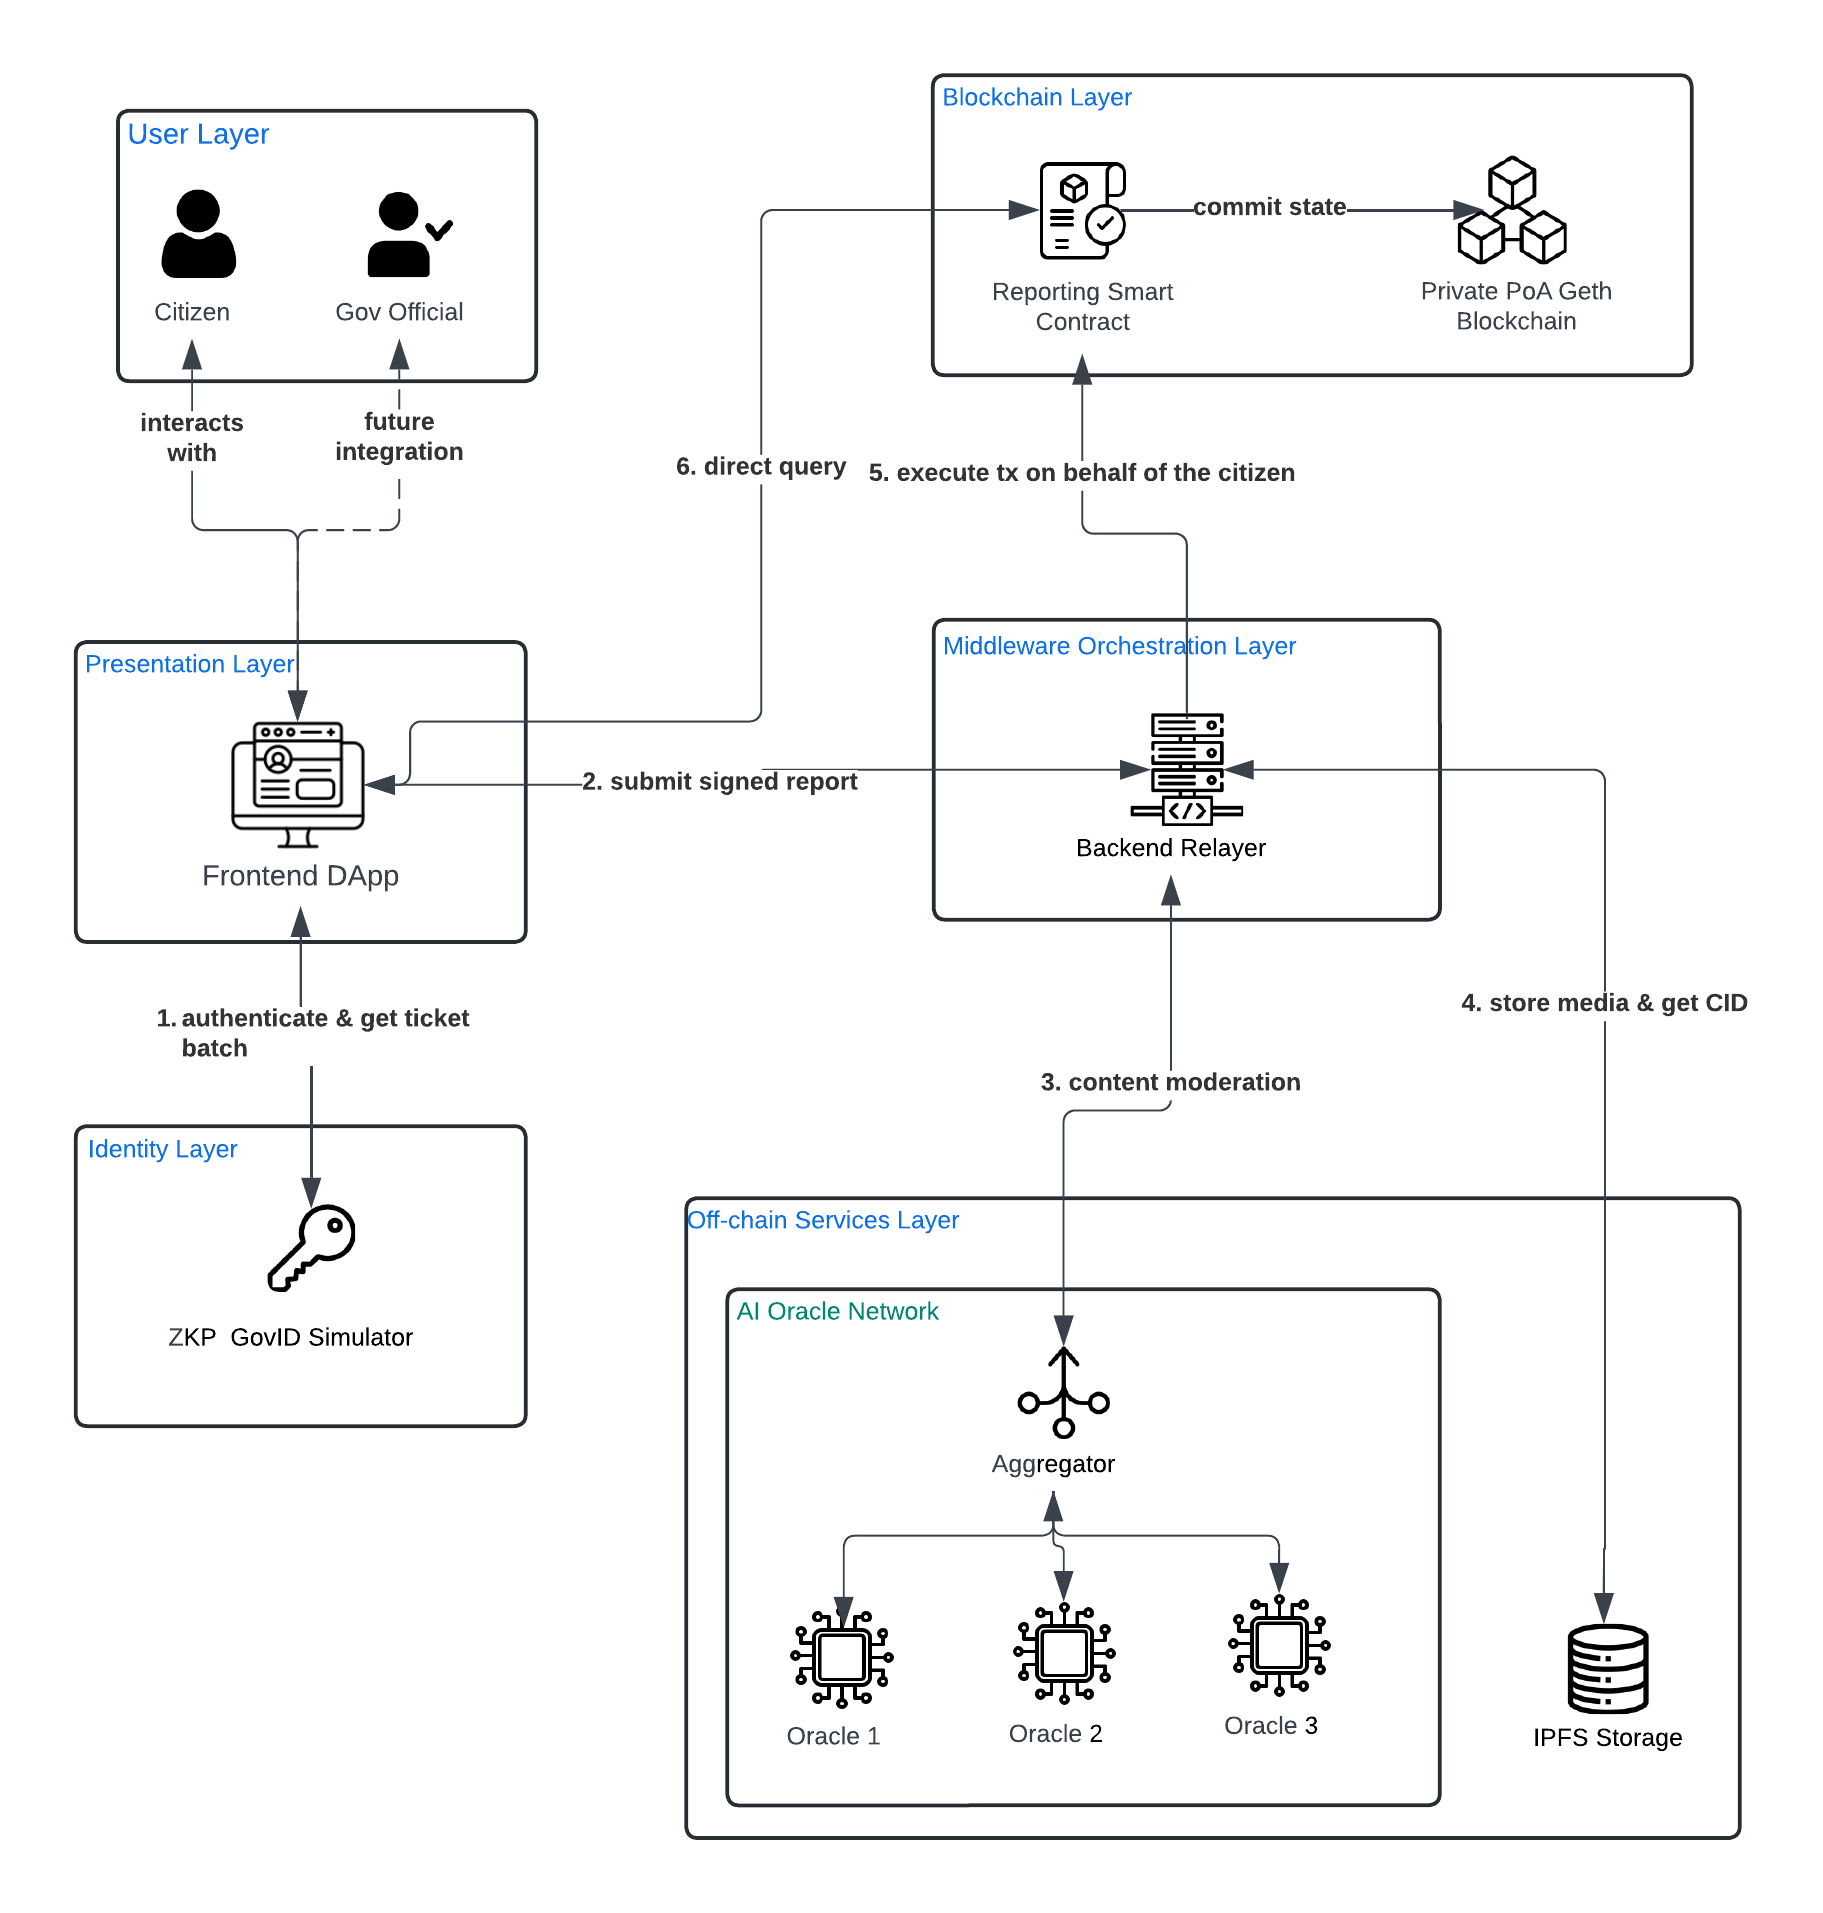
\includegraphics[width=0.95\textwidth,height=0.75\textheight,keepaspectratio]{Images/Chapter_3/overall-architecture.png}
    \caption{High-Level Architectural Diagram of the Proposed System}
    \label{fig:overall-architecture}
\end{figure}

Citizen identities are kept confidential. At the same time, all submitted reports, votes, authority responses, and governance role assignments are publicly verifiable and cannot be altered.

\subsection{Six-Layer Architectural Topology}
\label{subsec:six-layer-topology}

The architecture is divided into six layers. Each layer has specific responsibilities and provides standard interfaces to adjacent layers:

\begin{enumerate}
    \item \textbf{User Layer:} Contains the main actors: citizens, municipal authority workers, and approved institutional stakeholders such as \ac{NGO}s. Citizens submit reports and cast validation votes. Authorities claim and resolve reported issues. Municipal Super Admins oversee all governance operations.

    \item \textbf{Presentation (DApp) Layer:} A responsive, web-based \ac{DApp} built with Next.js and React. Citizens use it to authenticate, submit reports, upload media, browse the community feed, and vote anonymously. Authorities and Super Admins use it to manage open reports, post progress updates, and submit or vote on governance proposals. The DApp hides all blockchain complexity. Citizens do not need cryptocurrency wallets or gas fees.

    \item \textbf{Identity and Authentication Layer:} This layer verifies citizen credentials and issues cryptographic proof of eligibility without linking personal data to on-chain activity. The \ac{ZKP} GovID Simulator authenticates citizens against an official municipal registry and produces batches of single-use ticket identifiers (\texttt{zkpTicketId}), signed by the government and accompanied by a unique citizen seed. This prevents Sybil attacks while keeping identity fully decoupled from on-chain actions.

    \item \textbf{Middleware Orchestration (Relayer) Layer:} The backend relayer is the gateway between the DApp and the blockchain. It is built with NestJS. When a report is submitted, the relayer verifies two cryptographic signatures, forwards content to the AI moderation service, uploads accepted content to \ac{IPFS}, and submits gas-sponsored transactions to the blockchain on behalf of the citizen. It also funds newly approved authority wallets automatically and runs background cron jobs to finalise expired voting windows.

    \item \textbf{Off-Chain Services Layer:} Hosts two specialised services:
    \begin{itemize}
        \item \textit{AI Content Moderation Ensemble:} A multi-oracle machine learning service that checks report text and images for spam, toxicity, abuse, and civic relevance before on-chain anchoring.
        \item \textit{IPFS Distributed Storage:} A peer-to-peer storage network that stores report descriptions, images, and completion evidence. It returns an immutable \ac{CID} that is recorded on-chain.
    \end{itemize}

    \item \textbf{Blockchain Ledger Layer:} A private, permissioned blockchain running the Clique \ac{PoA} consensus engine. It executes the smart contract suite—\texttt{Reporting.sol}, \texttt{EmergencyReporting.sol}, \texttt{OpinionPolling.sol}, and \texttt{AuthorityMultiSig.sol}—which enforce lifecycle rules, manage access control, track one-time ticket nullifiers, and record an append-only audit trail of all governance events.
\end{enumerate}

\section{Subsystem Interconnection and Interaction Design}
\label{sec:subsystem-interconnection}

This section describes how the six architectural layers communicate and how security is enforced between them.

\subsection{Communication Protocols}
\label{subsec:comm-protocols}

Three primary protocol interfaces are used for inter-layer communication:
\begin{enumerate}
    \item \textbf{REST/HTTPS:} The \ac{DApp} communicates with the ZKP GovID Simulator and the Backend Relayer over HTTPS using JSON payloads. All endpoints enforce rate-limiting, request validation, and transport-layer encryption.
    \item \textbf{JSON-RPC and WebSocket:} The relayer and AI oracle workers communicate with the private blockchain through Ethereum-compatible JSON-RPC and WebSocket connections. WebSocket providers enable real-time event streaming, so off-chain workers can subscribe to on-chain events such as \texttt{ReportCreated} and \texttt{ProposalExecuted} with sub-second latency.
    \item \textbf{IPFS HTTP Gateway and RPC API:} The relayer pins files and retrieves metadata through the local IPFS daemon's RPC API (port 5001). Media is rendered on the client side using the IPFS HTTP gateway.
\end{enumerate}

\subsection{Dual-Layer Cryptographic Verification Engine}
\label{subsec:dual-layer-verification}

The Backend Relayer uses a dual-layer cryptographic verification engine. This allows citizens to submit reports without interacting with the blockchain directly, while also preventing unauthorized submissions and payload tampering. Two signatures are checked before any off-chain storage or on-chain transaction is executed:

\begin{enumerate}
    \item \textbf{Government Ticket Authenticity:} The relayer verifies the cryptographic signature on the ticket (\texttt{zkpTicketId}) using the government authority's ECDSA public key. This confirms the submitter is a verified citizen and that the ticket has not been forged.
    \item \textbf{Citizen Payload Integrity:} The relayer verifies the ECDSA signature that the citizen has signed over the composite report hash:
    \begin{equation}
        \mathcal{H}_{\text{report}} = \text{keccak256}\Big(\text{description} \parallel \text{zkpTicketId} \parallel \mathcal{H}_{\text{media}}\Big)
    \end{equation}
    This ensures that neither a man-in-the-middle attacker nor the relayer itself has altered the report description or the media evidence.
\end{enumerate}

Figure~\ref{fig:backend-relayer-impl} shows the internal architecture of the Backend Relayer.

\begin{figure}[!htbp]
    \centering
    \includegraphics[width=0.95\textwidth,height=0.75\textheight,keepaspectratio]{Images/Chapter 3/backend-relayer-impl.png}
    \caption{Backend Relayer Middleware Implementation and Verification Pipeline}
    \label{fig:backend-relayer-impl}
\end{figure}

\subsection{AI Moderation Oracle Ensemble}
\label{subsec:ai-oracle-interconnection}

Content moderation is carried out by a network of machine learning oracles. They filter out spam, harmful text, and non-civic content before anything is anchored on-chain. The network has four components:

\begin{enumerate}
    \item \textbf{Safety Oracle:} Uses \texttt{unitary/toxic-bert} to check text for abusive, hateful, or threatening language. Uses \texttt{Falconsai/nsfw\_image\_detection} to check images for unsafe content. Safe images with faces are processed through an OpenCV face-blurring pipeline before storage.
    \item \textbf{Spam and Abuse Oracle:} Uses \texttt{mrm8488/bert-tiny-finetuned-sms-spam-detection} combined with rule-based heuristics to detect promotional messages, gibberish, and repetitive spam patterns.
    \item \textbf{Civic Relevance Oracle:} Uses \texttt{sentence-transformers/all-MiniLM-L6-v2} to compute semantic embeddings of the report text. These embeddings are compared by cosine similarity against a predefined lexicon of municipal infrastructure categories to reject irrelevant submissions.
    \item \textbf{Oracle Aggregator:} The central verification gateway. It gathers signed moderation decisions from all three oracle workers, checks nonces and timestamps to prevent replay attacks, enforces an immediate rejection override when the Safety Oracle detects a critical violation, and applies majority voting to arrive at a final \texttt{ACCEPT} or \texttt{REJECT} decision.
\end{enumerate}

Figure~\ref{fig:oracle-architecture} shows the oracle ensemble topology.

\begin{figure}[!htbp]
    \centering
    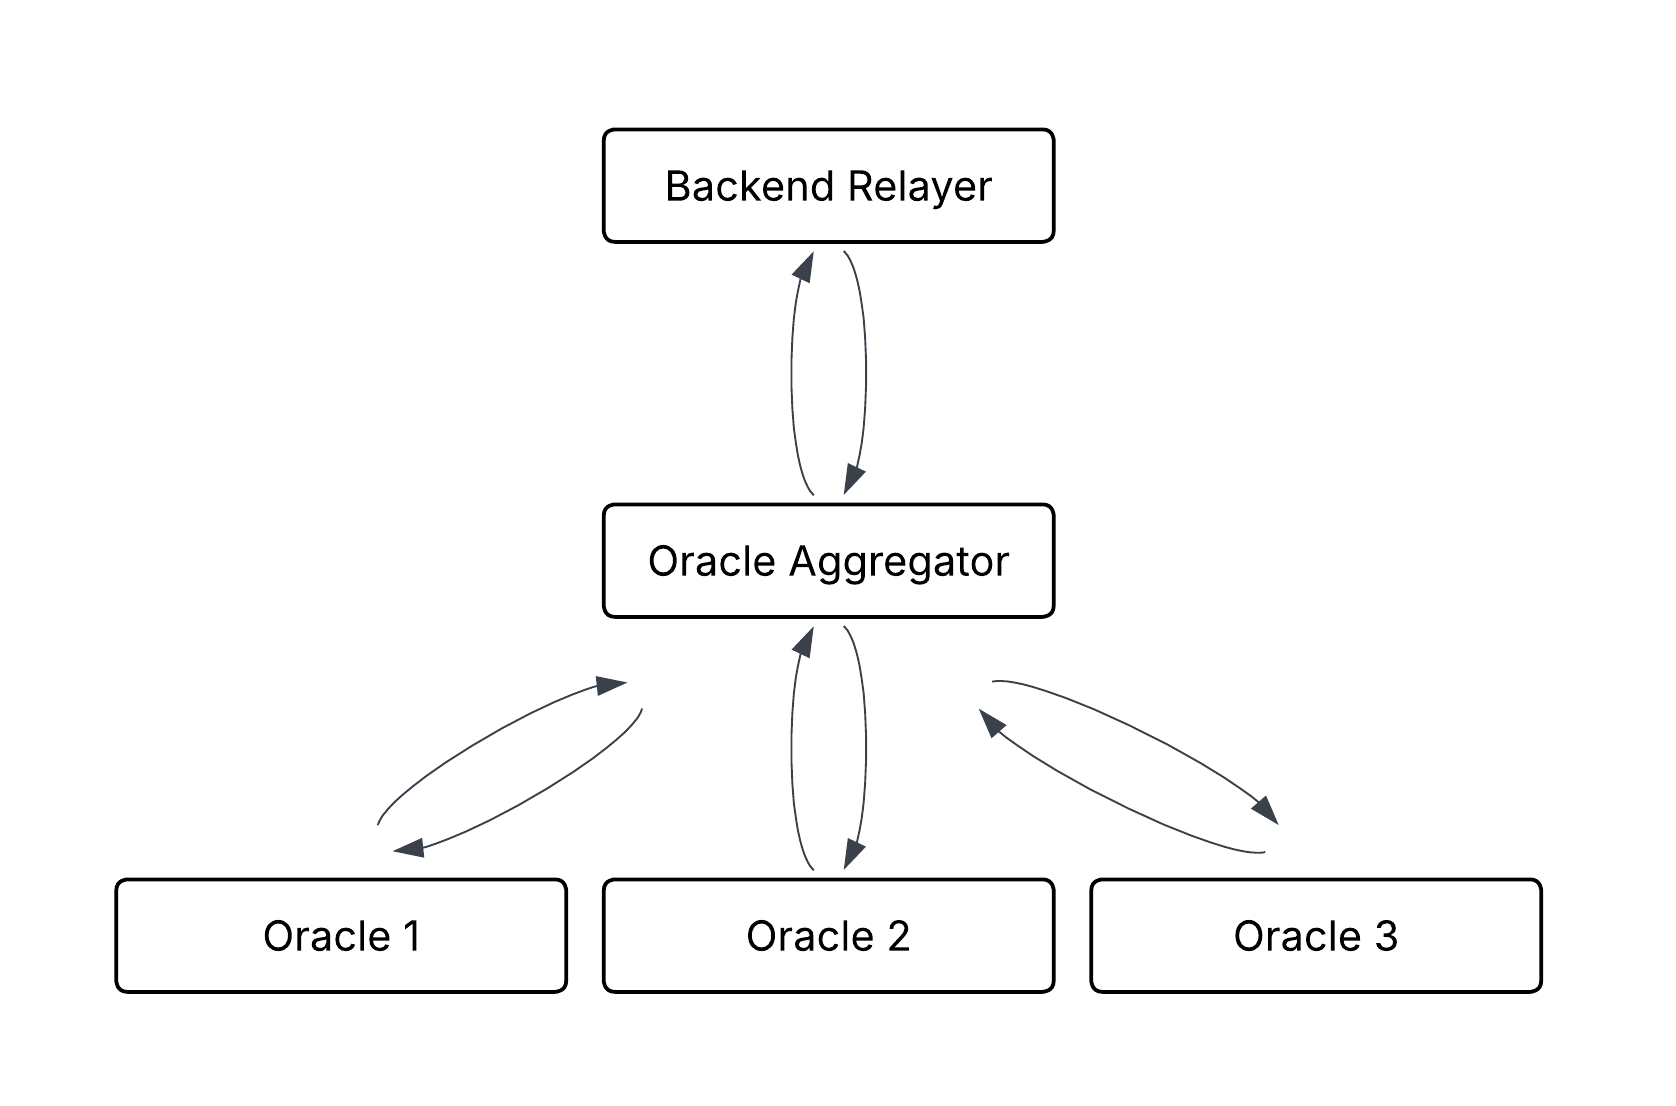
\includegraphics[width=0.95\textwidth,height=0.75\textheight,keepaspectratio]{Images/Chapter_3/oracle-architecture.png}
    \caption{AI Content Moderation Ensemble and Oracle Aggregator Topology}
    \label{fig:oracle-architecture}
\end{figure}

\subsection{Two-Tier Multi-Signature Governance and Access Control}
\label{subsec:multisig-governance}

Access control is managed by a two-tier multi-signature governance contract, \texttt{AuthorityMultiSig.sol}. Ownership of \texttt{Reporting.sol} is transferred to this contract at deployment. This prevents any single administrator from abusing their power. Two tiers of stakeholders are defined:

\begin{enumerate}
    \item \textbf{Super Admins:} Senior municipal officials (such as the Mayor, Deputy Mayor, CEO, and Town Planner) who manage the ecosystem. Only Super Admins can submit and vote on governance proposals. The quorum is computed dynamically as a simple majority of the current Super Admin count:
    \begin{equation}
        \text{Quorum} = \Big\lfloor \frac{\texttt{superAdminCount}}{2} \Big\rfloor + 1
    \end{equation}
    A proposal executes automatically once quorum is reached.
    \item \textbf{Authority Workers:} Municipal engineering and maintenance staff who are authorized to act on civic issues in \texttt{Reporting.sol} (calling \texttt{startWork}, \texttt{addAuthorityUpdate}, \texttt{markAsSolved}, and \texttt{rejectIssue}). Access can only be granted or revoked through Super Admin multi-sig proposals (\texttt{AddAuthority} and \texttt{RemoveAuthority}).
    \item \textbf{On-Chain Profile Directory:} Each Super Admin and Authority Worker has an immutable on-chain identity profile (\texttt{Profile} struct) that stores their full name, official title, and municipal department. Citizens can check who is assigned to a report directly from the DApp.
\end{enumerate}

When an \texttt{AddAuthority} or \texttt{RemoveAuthority} proposal reaches quorum, \texttt{AuthorityMultiSig.sol} calls \texttt{IReporting.setAuthority(target, authorized)}, immediately updating the access registry on the main reporting contract.

\subsection{Automated Relayer Funding and Cron Orchestration}
\label{subsec:relayer-funding-cron}

The Backend Relayer includes two automation services that connect on-chain governance with off-chain operational readiness:

\begin{enumerate}
    \item \textbf{Authority Funding Service (\texttt{AuthorityFundingService}):} When a new authority is added through governance, they need native ETH to pay gas fees on the PoA blockchain. The funding service listens for \texttt{ProposalExecuted} events via WebSocket. When an \texttt{AddAuthority} proposal executes, the service automatically transfers a configurable top-up balance (default: 5.0 ETH) from the relayer treasury to the new authority's wallet.

    \item \textbf{Background Cron Service (\texttt{CronService}):} Two scheduled jobs run in the background:
    \begin{itemize}
        \item \textit{Balance Monitoring:} Every day at 01:00 Colombo time, the balances of all registered Super Admins and Authority Workers are checked. Any account that falls below the minimum operating threshold (1.0 ETH) is topped up automatically.
        \item \textit{Voting Window Batch Finalization:} Reports that receive no new votes can remain in a voting state indefinitely. To prevent this, a daily midnight cron job identifies reports in voting phases ($S_0$, $S_4$, or $S_5$) where \texttt{block.timestamp > phaseDeadline} and calls \texttt{batchFinalizeVotingWindows}, forcing deterministic state transitions.
    \end{itemize}
\end{enumerate}

\subsection{Asynchronous Job Queue Architecture}
\label{subsec:async-queue}

Report submission involves three sequential steps: AI moderation, IPFS upload, and blockchain transaction submission. If these steps run synchronously inside a single HTTP request, the citizen must wait for the entire pipeline before receiving any response. This creates unacceptable latency.

To solve this, the Backend Relayer uses a BullMQ job queue backed by Redis. BullMQ is a Node.js queue library that supports persistent, distributed job processing with retry policies and job dependency graphs. Redis acts as the durable message broker — queued jobs are not lost even if the relayer restarts.

The queue uses the \textbf{BullMQ Flow API}. When a report is submitted, the relayer enqueues a \textbf{Flow Job} — a parent job containing three ordered child jobs:

\begin{enumerate}
    \item \textbf{Step 1 — AI Moderation} (\texttt{step1-ai-moderation}): The AI oracle ensemble assesses the report text and images. This is the leaf node and executes first.
    \item \textbf{Step 2 — IPFS Upload} (\texttt{step2-ipfs-upload}): The report content is uploaded to IPFS. This step reads the AI verdict from the parent result store using \texttt{getChildrenValues()}.
    \item \textbf{Step 3 — Blockchain Submission} (\texttt{step3-blockchain-submit}): The IPFS CID and cryptographic metadata are submitted to \texttt{Reporting.sol}. This step depends on the result of Step 2.
    \item \textbf{Parent Summary Job:} After all child steps complete, the parent job aggregates the final result and emits the \texttt{completed} progress event.
\end{enumerate}

Each child job is configured with \texttt{failParentOnFailure: true}. If any step fails, the entire flow is marked as failed. Each step uses an exponential-backoff retry policy with a maximum of three attempts:
\begin{equation}
    \Delta t_{\text{retry}}(k) = t_{\text{base}} \times 4^{k-1}, \quad k \in \{1, 2, 3\}
\end{equation}
where $t_{\text{base}} = 2{,}000\,\text{ms}$, giving retry delays of 2\,s, 8\,s, and 32\,s.

Job identifiers follow the naming convention: the parent job uses \texttt{rpt\_<ticketHash>}, and the child steps use \texttt{rpt\_<ticketHash>-ai}, \texttt{rpt\_<ticketHash>-ipfs}, and \texttt{rpt\_<ticketHash>-chain}. This makes individual pipeline steps easy to track and debug.

A separate \textbf{Vote Queue} (\texttt{vote-queue}) is used to process community vote submissions asynchronously.

Figure~\ref{fig:queue-architecture} shows the BullMQ Flow job tree.

\begin{figure}[!htbp]
    \centering
    \fbox{\parbox{0.85\textwidth}{\centering\vspace{1.5cm}
    \textit{[Image suggestion IMG-03: BullMQ Flow Job Tree Diagram showing the parent job containing three ordered child steps (AI, IPFS, Blockchain), Redis as the broker, and arrows indicating dependency order with retry logic labels.]}
    \vspace{1.5cm}}}
    \caption{BullMQ Flow Job Architecture for Asynchronous Report Submission Processing}
    \label{fig:queue-architecture}
\end{figure}

\subsection{Real-Time Status Notification via Server-Sent Events (SSE)}
\label{subsec:sse-gateway}

Once a report is accepted and enqueued, the citizen's DApp does not wait for a blocking HTTP response. Instead, the DApp opens a persistent \ac{SSE} connection to the Backend Relayer to receive real-time progress updates as each pipeline step completes.

The notification system works as follows:

\begin{enumerate}
    \item \textbf{Queue worker progress emission:} At each pipeline stage, the queue worker emits a structured \texttt{ReportJobProgress} event through the NestJS \texttt{EventEmitter2} event bus.
    \item \textbf{SSE Subject bridge:} The \texttt{ReportStatusGateway} controller subscribes to these internal events using the \texttt{@OnEvent} decorator. Each event is forwarded into an RxJS \texttt{Subject}, which acts as a push-based observable stream.
    \item \textbf{Citizen-scoped SSE stream:} The DApp connects to \texttt{GET /report/status/stream?citizenAddress=<address>}. The SSE stream applies an RxJS \texttt{filter} to forward only events where \texttt{citizenPubKey} matches the connected citizen's address. This ensures that each citizen receives only their own job updates.
    \item \textbf{Progress payload:} Each SSE event carries a structured payload containing the \texttt{jobId}, the current pipeline \texttt{step}, a \texttt{percent} value (0--100), a human-readable \texttt{message}, and optional extra data such as the IPFS CID or transaction hash.
\end{enumerate}

Two additional HTTP endpoints support page-refresh recovery:
\begin{itemize}
    \item \texttt{GET /report/status/citizen/:address} — returns the current state of all jobs for a citizen (waiting, active, completed, or failed).
    \item \texttt{GET /report/status/:jobId} — returns the status of a specific job.
\end{itemize}

The defined progress steps are: \texttt{pending}, \texttt{ai\_moderation\_in\_progress}, \texttt{ai\_moderation\_passed}, \texttt{ai\_moderation\_failed}, \texttt{ipfs\_uploading}, \texttt{ipfs\_uploaded}, \texttt{ipfs\_failed}, \texttt{blockchain\_submitting}, \texttt{blockchain\_submitted}, \texttt{blockchain\_failed}, and \texttt{completed}.

Citizens receive immediate confirmation that their report is queued, followed by step-by-step progress updates without refreshing the page. The DApp renders these as a visual progress bar.

\subsection{Private Permissioned Validator Network Topology}
\label{subsec:validator-topology}

The blockchain runs as a private, permissioned network using the Clique \ac{PoA} consensus protocol. Block sealing authority is limited to three pre-approved institutional validator nodes:

\begin{itemize}
    \item \textbf{Municipal Authority Validator Node:} Hosted by the local government administrative department.
    \item \textbf{Regional Oversight Validator Node:} Managed by a regional or provincial supervisory body for inter-agency auditing.
    \item \textbf{Independent Civic NGO Validator Node:} Operated by a recognized civil society organization to maintain democratic balance and prevent unilateral censorship by government nodes.
\end{itemize}

Figure~\ref{fig:validator-nodes} shows the 3-validator network topology.

\begin{figure}[!htbp]
    \centering
    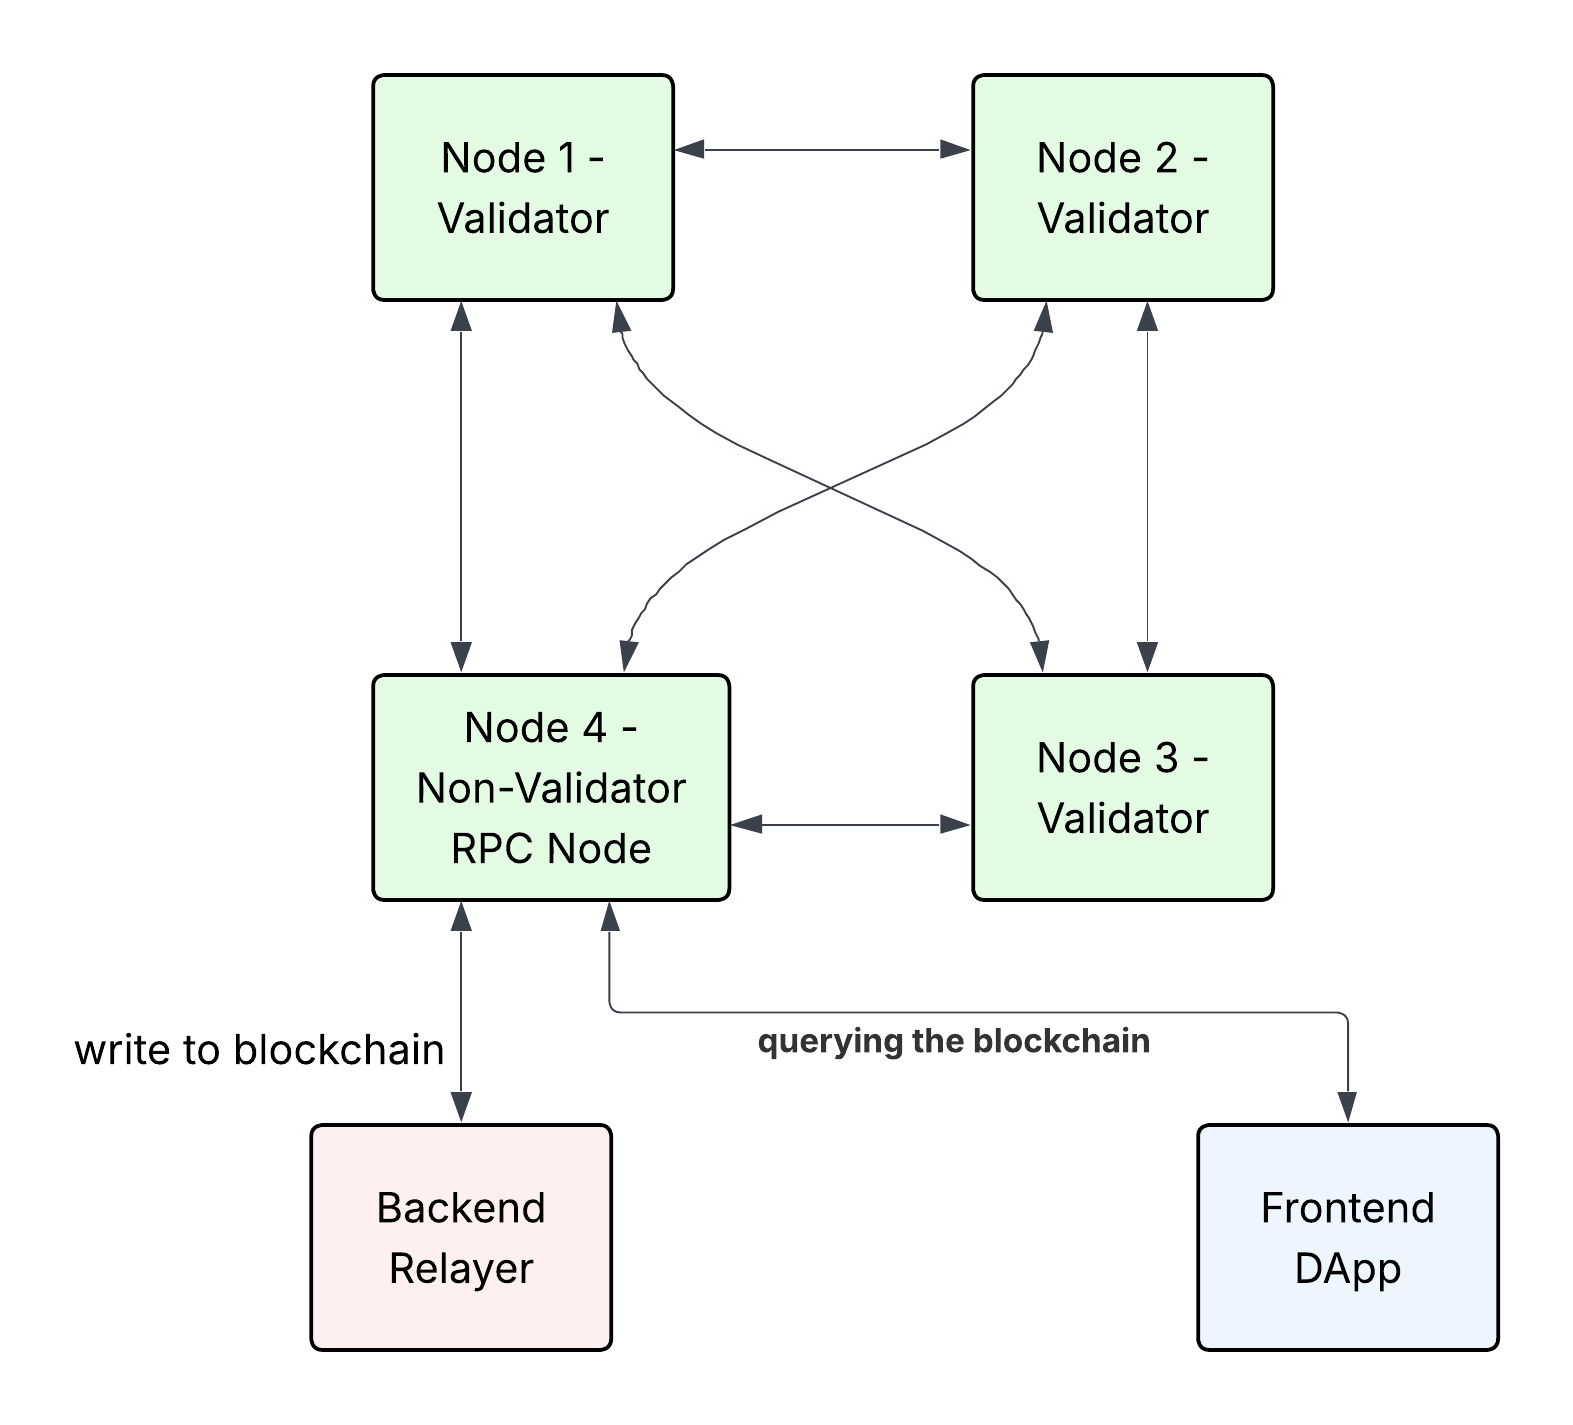
\includegraphics[width=0.95\textwidth,height=0.75\textheight,keepaspectratio]{Images/Chapter 3/validator_nodes.png}
    \caption{Private Permissioned Proof-of-Authority (PoA) Validator Network Topology}
    \label{fig:validator-nodes}
\end{figure}

\section{Detailed Workflow and Finite State Machine (FSM) Design}
\label{sec:detailed-workflow-fsm}

The operational logic of the platform is expressed as a deterministic \ac{FSM} implemented in \texttt{Reporting.sol}. This section describes the state transitions, nullifier safeguards, and workflows that govern a civic report from submission to final verification.

\subsection{Finite State Machine (FSM) Overview}
\label{subsec:fsm-overview}

A civic issue report is modeled as an eight-state deterministic \ac{FSM}. The set of legal states is:
\begin{equation}
    \mathcal{S} = \big\{ S_0, S_1, S_2, S_3, S_4, S_5, S_6, S_7 \big\}
\end{equation}
where:
\begin{itemize}
    \item $S_0 = \texttt{PendingValidation}$: The initial state after on-chain submission. The report is visible on the community feed for peer validation voting within a 6-hour window.
    \item $S_1 = \texttt{CommunityRejected}$: A terminal state. Downvotes exceed upvotes during the validation phase.
    \item $S_2 = \texttt{Open}$: Community consensus is reached. The issue is now actionable for municipal authorities.
    \item $S_3 = \texttt{InProgress}$: An assigned authority has claimed the report and started physical repairs.
    \item $S_4 = \texttt{PendingRejectionReview}$: An authority has rejected the issue. The community has 6 hours to uphold or appeal the rejection.
    \item $S_5 = \texttt{PendingVerification}$: An authority has marked the issue as solved. Citizens inspect the repair and cast accept or reject votes within a 6-hour window.
    \item $S_6 = \texttt{Closed}$: A terminal state. The issue has been resolved and community-verified, or a rejection has been upheld.
    \item $S_7 = \texttt{Reopened}$: The community has rejected a claimed repair, or successfully appealed an authority rejection.
\end{itemize}

State transitions are protected by \ac{RBAC}, time window constraints ($\Delta t_{\text{window}} = 6\text{ hours}$), and cryptographic nullifier tracking. To prevent Sybil attacks and double voting, the smart contract maintains four permanent mappings (\texttt{usedSubmissionNullifiers}, \texttt{usedValidationVoteNullifiers}, \texttt{usedVerificationVoteNullifiers}, and \texttt{usedRejectionReviewVoteNullifiers}) following the Checks-Effects-Interactions (CEI) pattern.

Figure~\ref{fig:state-transition-diagram} shows the formal state transition diagram. Figure~\ref{fig:overall-workflow} shows the end-to-end lifecycle workflow.

\begin{figure}[!htbp]
    \centering
    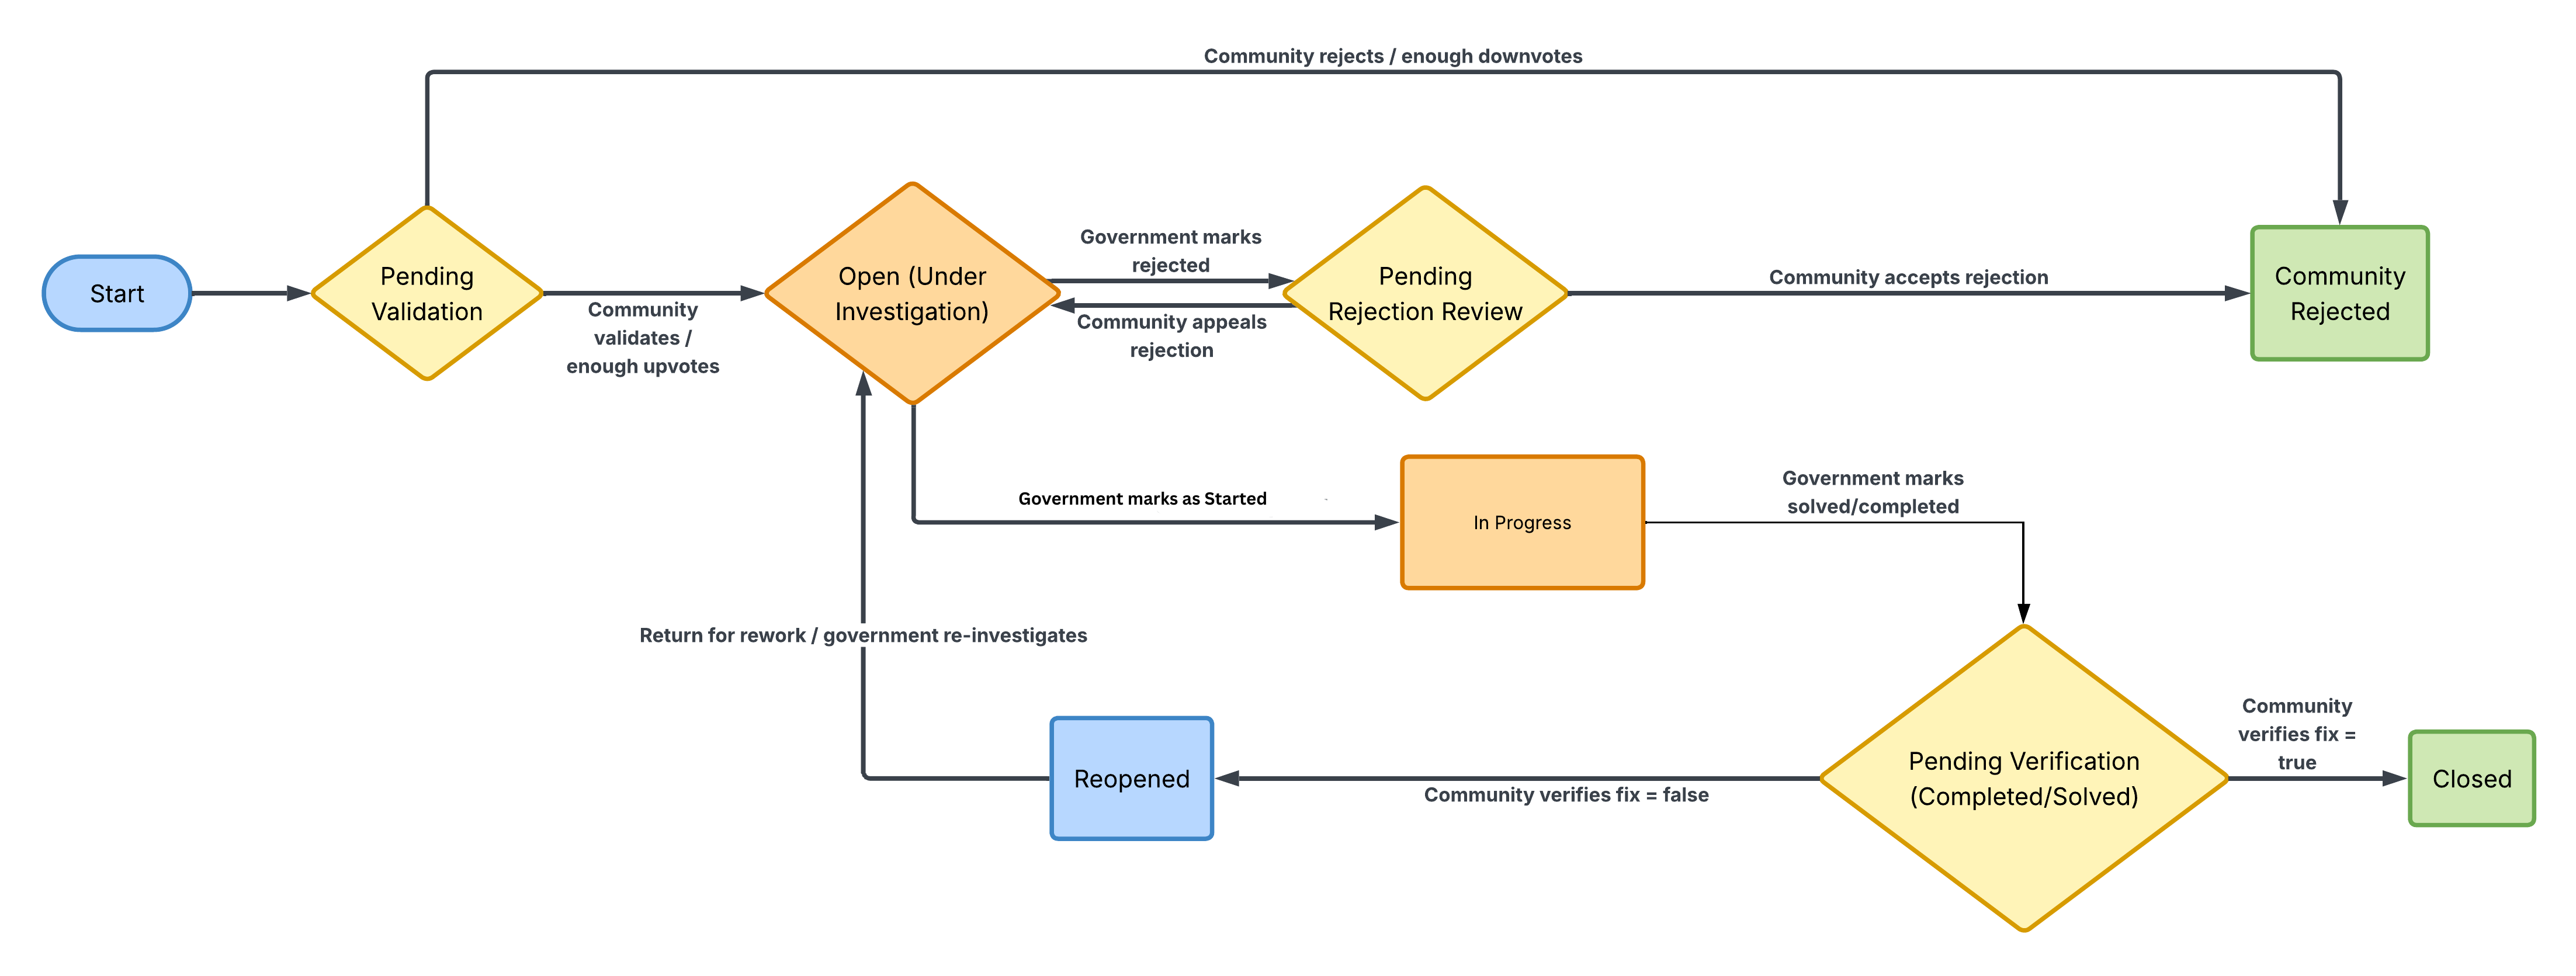
\includegraphics[width=0.95\textwidth,height=0.75\textheight,keepaspectratio]{Images/Chapter 3/state-transition-diagram-3.png}
    \caption{Finite State Machine (FSM) State Transition Diagram for Civic Reports}
    \label{fig:state-transition-diagram}
\end{figure}

\begin{figure}[!htbp]
    \centering
    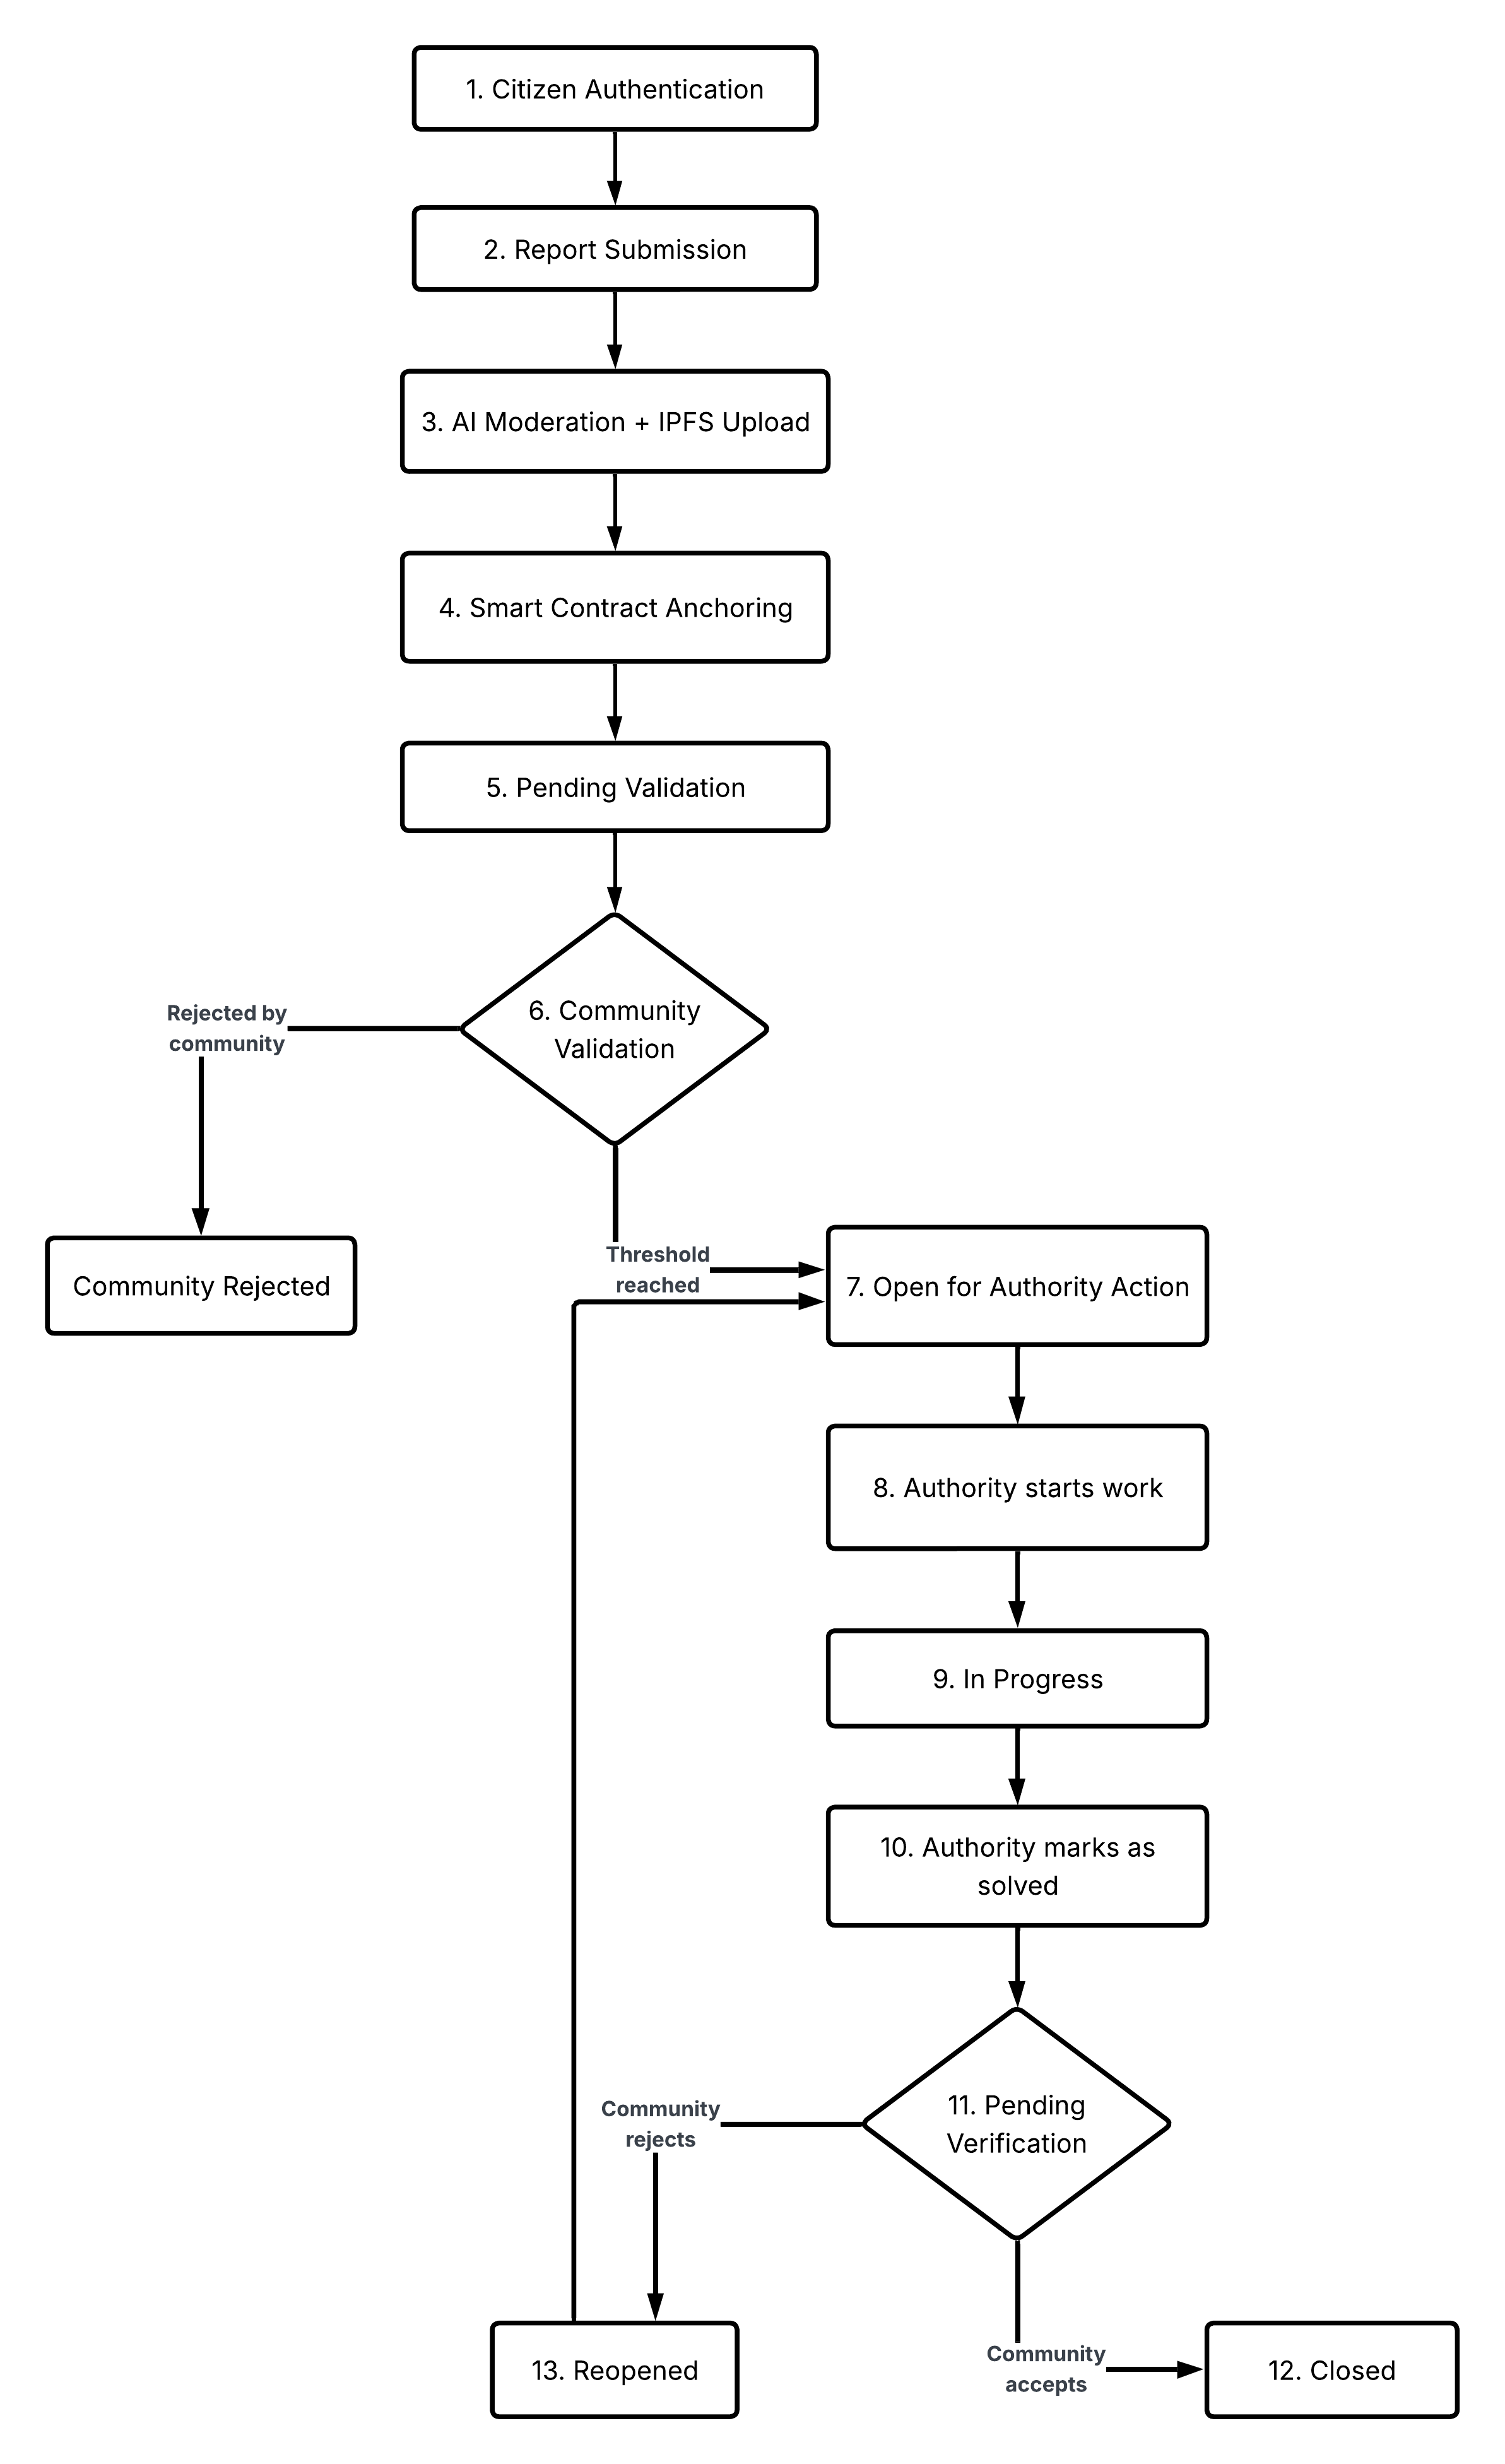
\includegraphics[width=0.95\textwidth,height=0.75\textheight,keepaspectratio]{Images/Chapter 3/overall_reporting_workflow.png}
    \caption{Overall Lifecycle Workflow of a Civic Issue Within the Decentralized Ecosystem}
    \label{fig:overall-workflow}
\end{figure}

\subsection{Citizen Authentication and Identity Decoupling Workflow}
\label{subsec:auth-workflow}

The authentication workflow separates a citizen's real-world identity from their on-chain actions. Figure~\ref{fig:authentication-workflow} shows the sequential steps in this process.

\begin{figure}[!htbp]
    \centering
    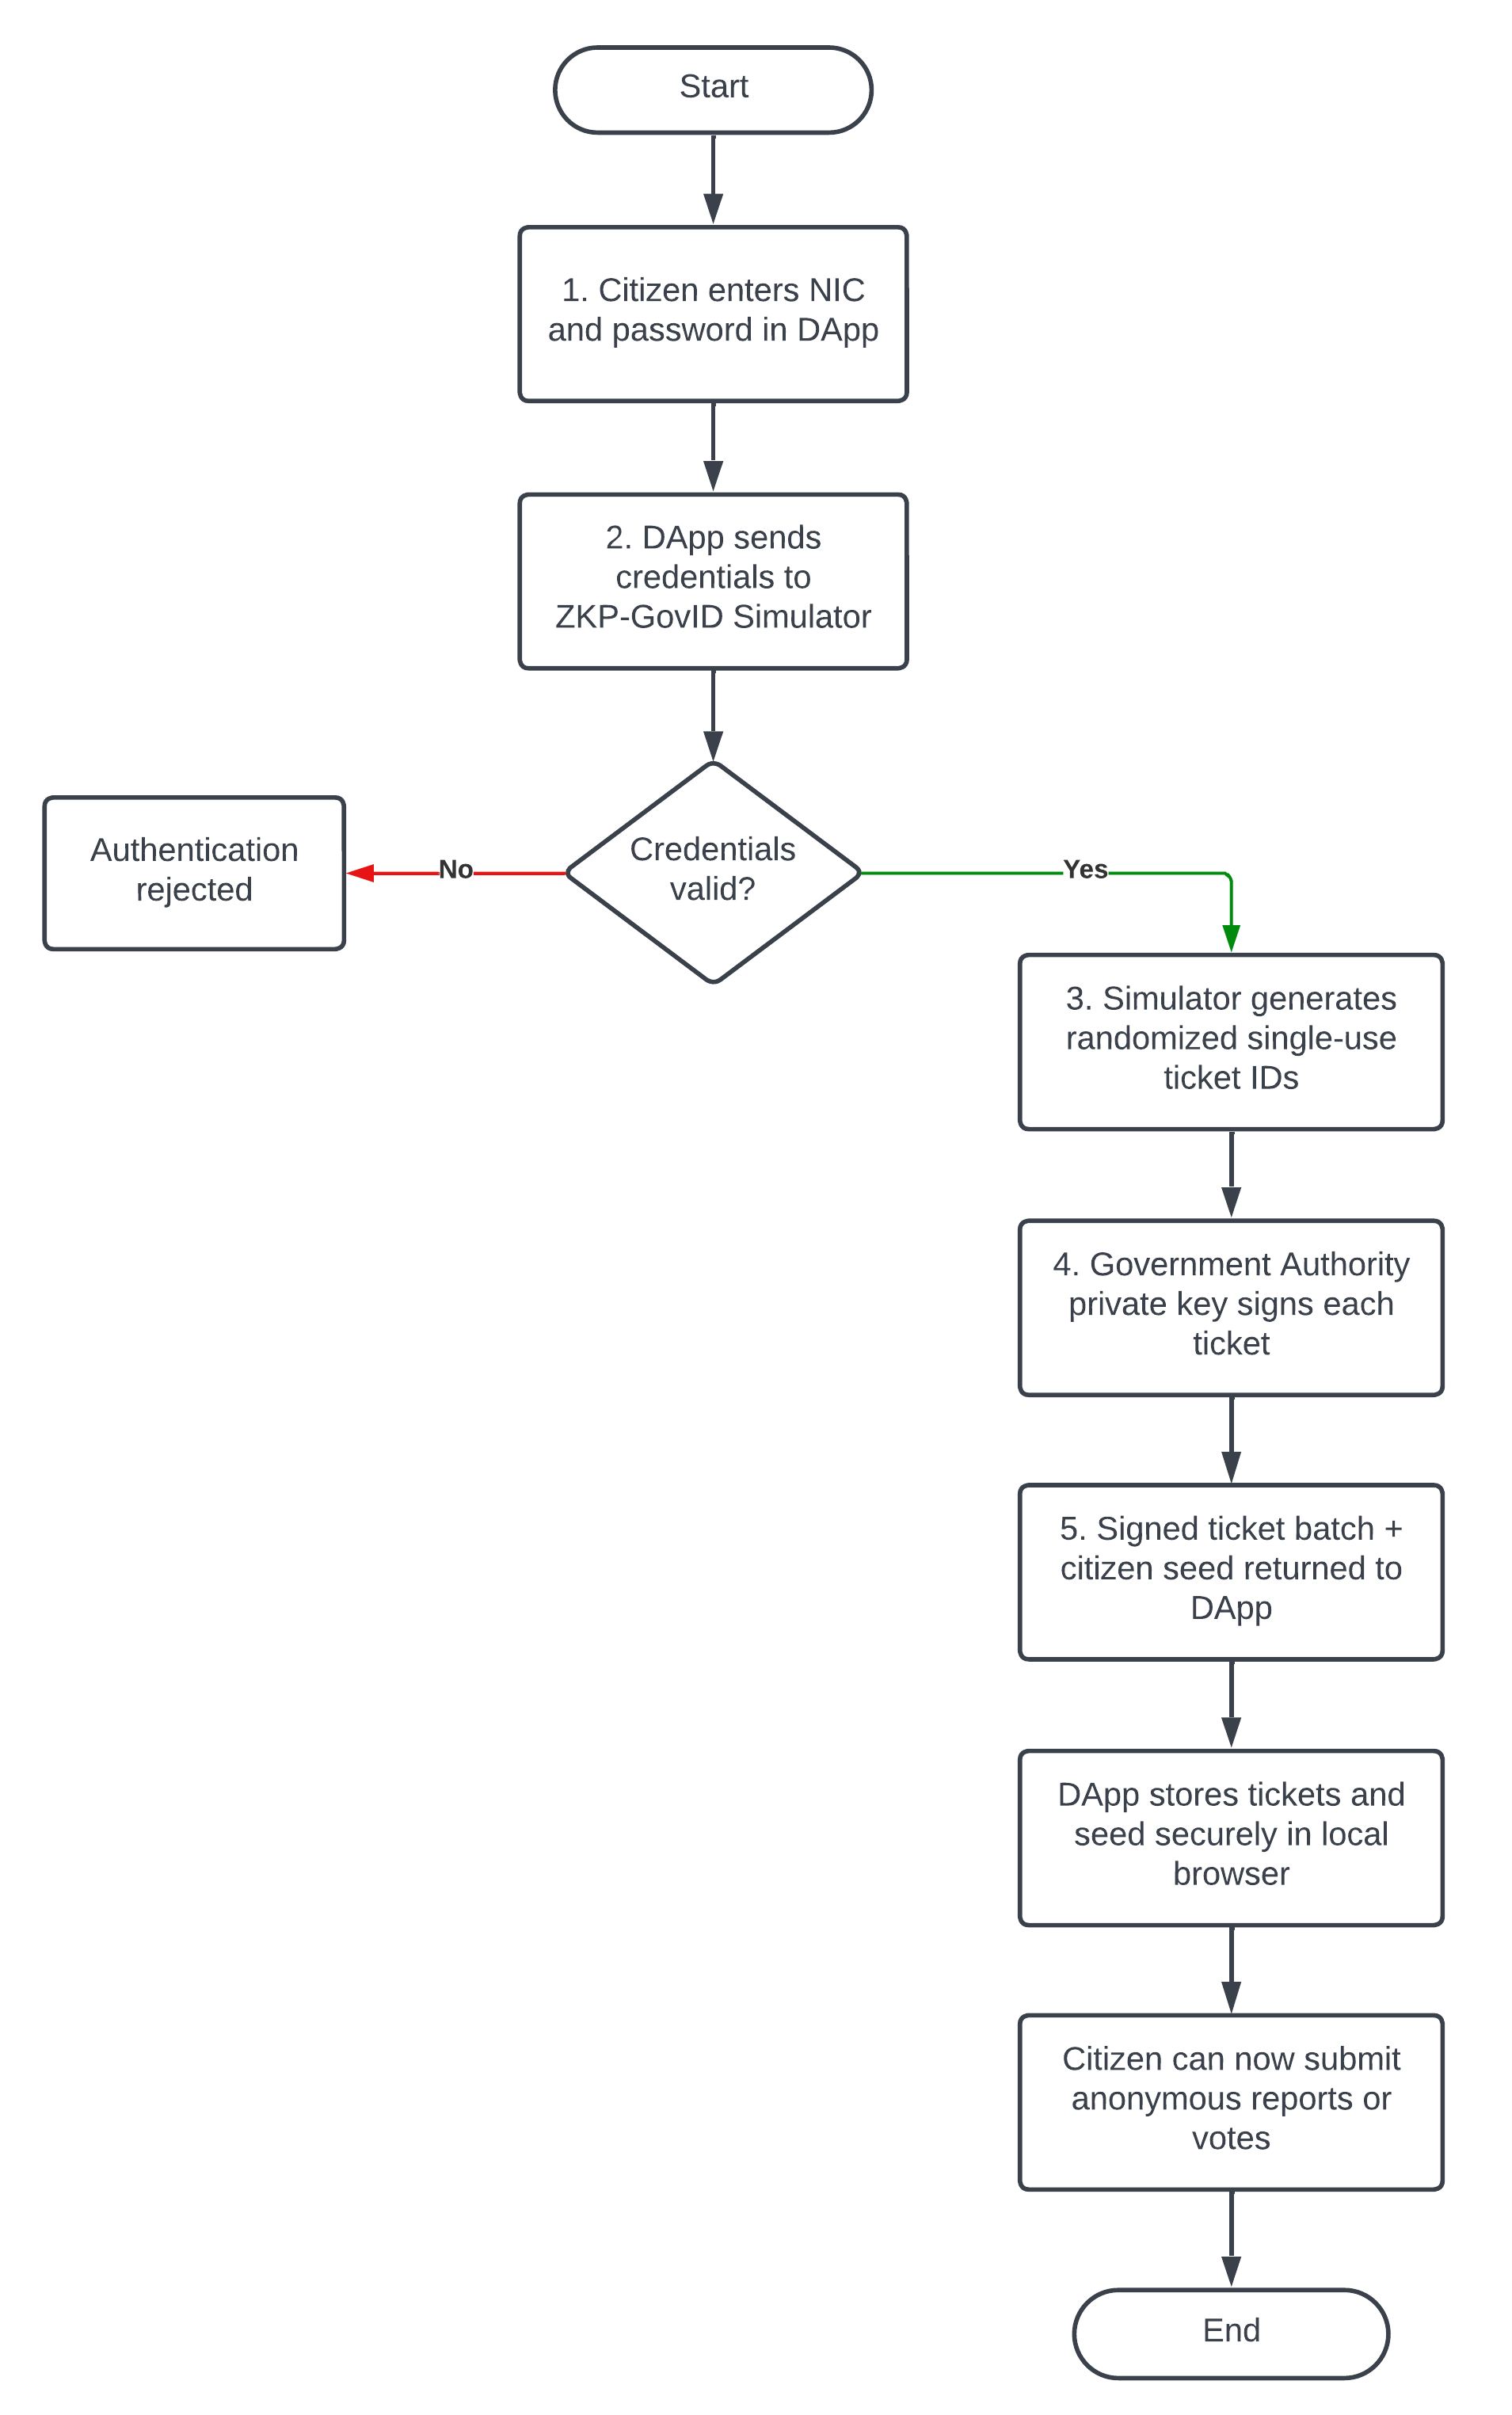
\includegraphics[width=0.95\textwidth,height=0.75\textheight,keepaspectratio]{Images/Chapter 3/authentication_workflow.png}
    \caption{Citizen Authentication and Identity Decoupling Workflow}
    \label{fig:authentication-workflow}
\end{figure}

The authentication workflow has five steps:
\begin{enumerate}
    \item \textbf{Credential Submission:} The citizen enters their National Identity Number (NID) and password into the DApp login interface.
    \item \textbf{Zero-Knowledge Verification:} The DApp sends an authentication request to the ZKP GovID Simulator. The simulator checks credentials against the government database without revealing or retaining any personal attributes.
    \item \textbf{Ticket Batch Generation:} After successful verification, the simulator produces a batch of ten randomly generated, single-use ticket identifiers ($\texttt{zkpTicketId}_1, \dots, \texttt{zkpTicketId}_{10}$) and a unique citizen seed.
    \item \textbf{Cryptographic Signing:} Each ticket identifier is signed by the simulator using the government authority's private key.
    \item \textbf{Local Browser Storage:} The signed ticket batch and citizen seed are stored securely in the browser's local storage. The client derives a deterministic, unlinkable citizen pseudonym:
    \begin{equation}
        \text{Pseudonym} = \text{keccak256}\Big(\text{citizenPubKey} \parallel \text{DOMAIN\_SALT}\Big)
    \end{equation}
\end{enumerate}

\subsection{Report Submission and Moderation Pipeline}
\label{subsec:submission-pipeline}

The report submission workflow involves client-side cryptographic signing, relayer verification, AI moderation, IPFS storage, and blockchain anchoring. Figure~\ref{fig:report-submission-workflow} shows the complete pipeline.

\begin{figure}[!htbp]
    \centering
    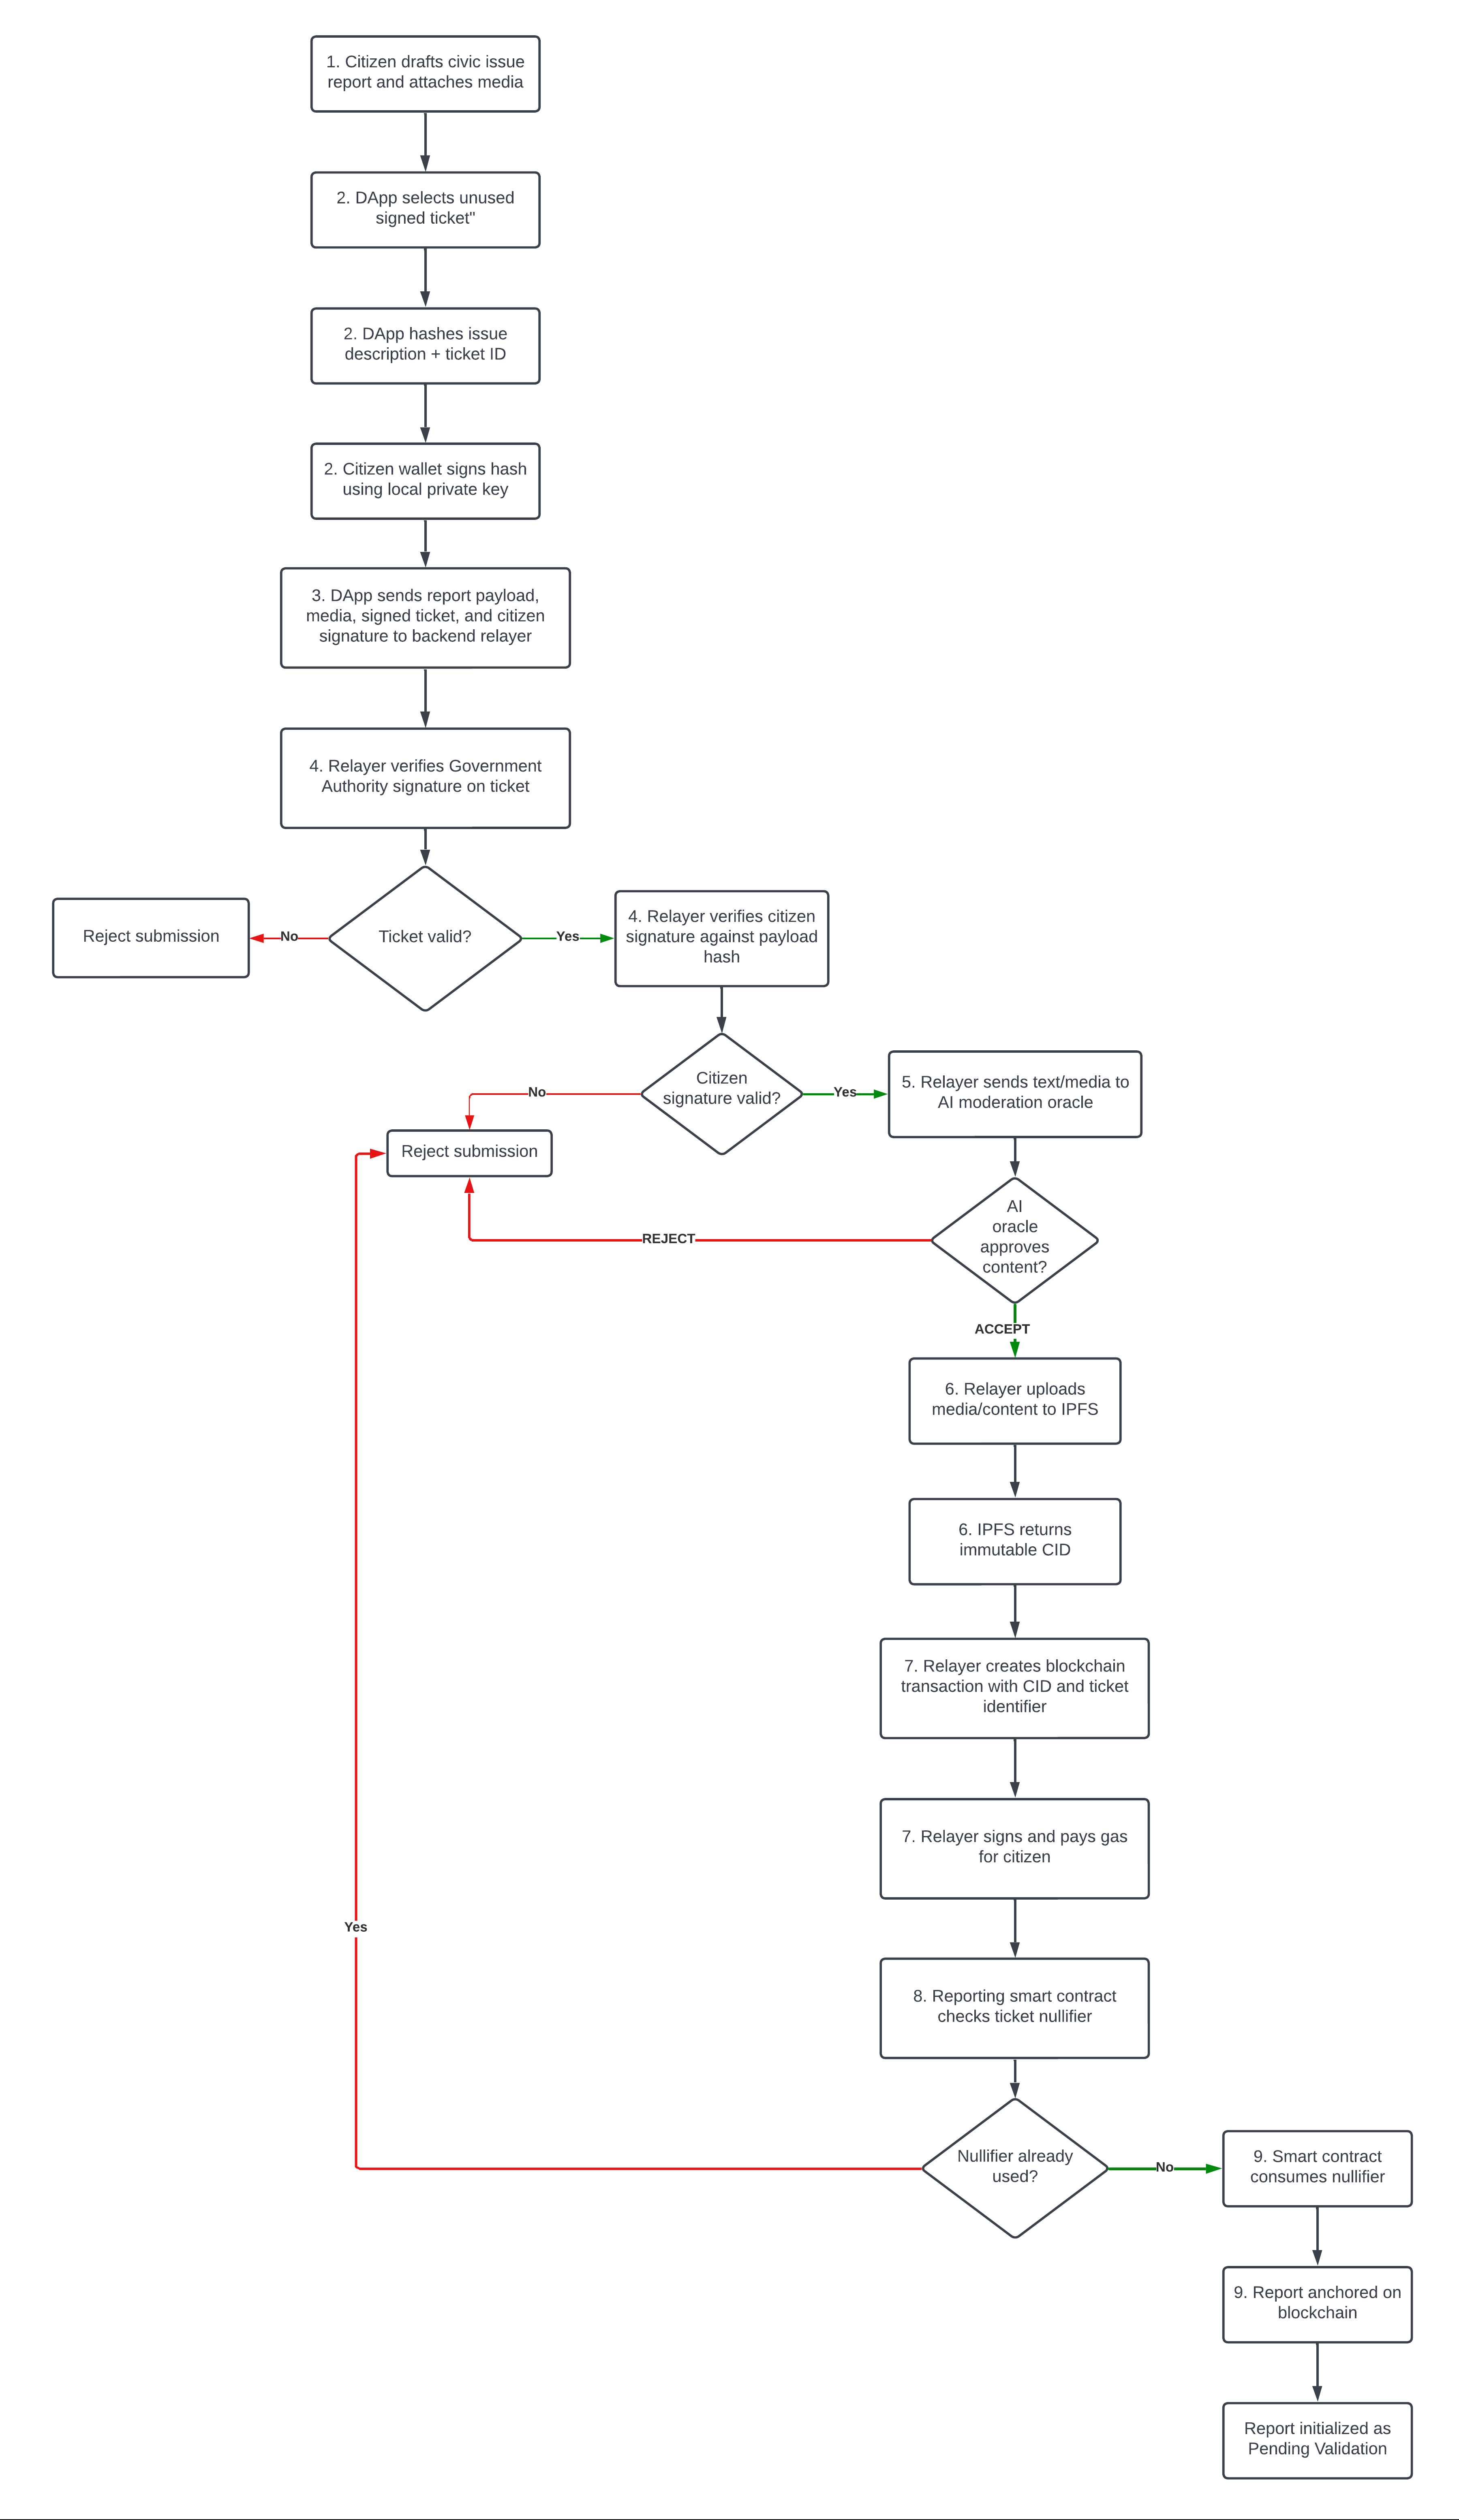
\includegraphics[width=0.95\textwidth,height=0.75\textheight,keepaspectratio]{Images/Chapter 3/report_submission_workflow.png}
    \caption{Report Submission, AI Moderation, and Blockchain Anchoring Pipeline}
    \label{fig:report-submission-workflow}
\end{figure}

The submission pipeline runs as follows:
\begin{enumerate}
    \item \textbf{Payload Structuring and Signing:} The citizen selects an issue category, types a description, and attaches optional media. The DApp computes the composite report hash ($\mathcal{H}_{\text{report}}$), signs it with the citizen's ephemeral private key, and selects an unused signed ticket.
    \item \textbf{Relayer Transmission:} The DApp sends the full payload — raw text, media files, the government-signed ticket, and the citizen's signature — to the Backend Relayer via HTTPS POST.
    \item \textbf{Cryptographic Payload Verification:} The relayer verifies that the ticket signature belongs to the government authority and that the citizen's signature matches the report hash. If verification fails, the request is rejected immediately.
    \item \textbf{AI Content Moderation:} The relayer forwards the text and media to the AI Moderation Ensemble. If the ensemble rejects the submission, the relayer aborts and returns a descriptive error to the DApp.
    \item \textbf{IPFS Content Anchoring:} On an \texttt{ACCEPT} verdict, the relayer uploads the report text and media to IPFS, obtaining the immutable Content Identifier (\texttt{ipfsCid}).
    \item \textbf{On-Chain Transaction Submission:} The relayer submits a transaction calling \texttt{submitReport} on \texttt{Reporting.sol}, passing the \texttt{ipfsCid}, $\mathcal{H}_{\text{report}}$, the ticket hash as the \texttt{submissionNullifier}, and the citizen's pseudonym. The relayer signs and pays the gas cost.
    \item \textbf{Smart Contract Nullifier Enforcement:} The smart contract checks \texttt{usedSubmissionNullifiers[submissionNullifier]}. If already used, the transaction reverts. Otherwise, the nullifier is recorded, the report is placed in state $S_0$, the phase deadline is set to $\text{block.timestamp} + 6\text{ hours}$, and the \texttt{ReportSubmitted} event is emitted.
\end{enumerate}

\subsection{Community Consensus and Validation Workflow}
\label{subsec:validation-workflow}

Newly submitted reports go through a community validation phase to filter spam and ensure only genuine civic concerns reach municipal authorities. Figure~\ref{fig:community-validation-workflow} shows this workflow.

\begin{figure}[!htbp]
    \centering
    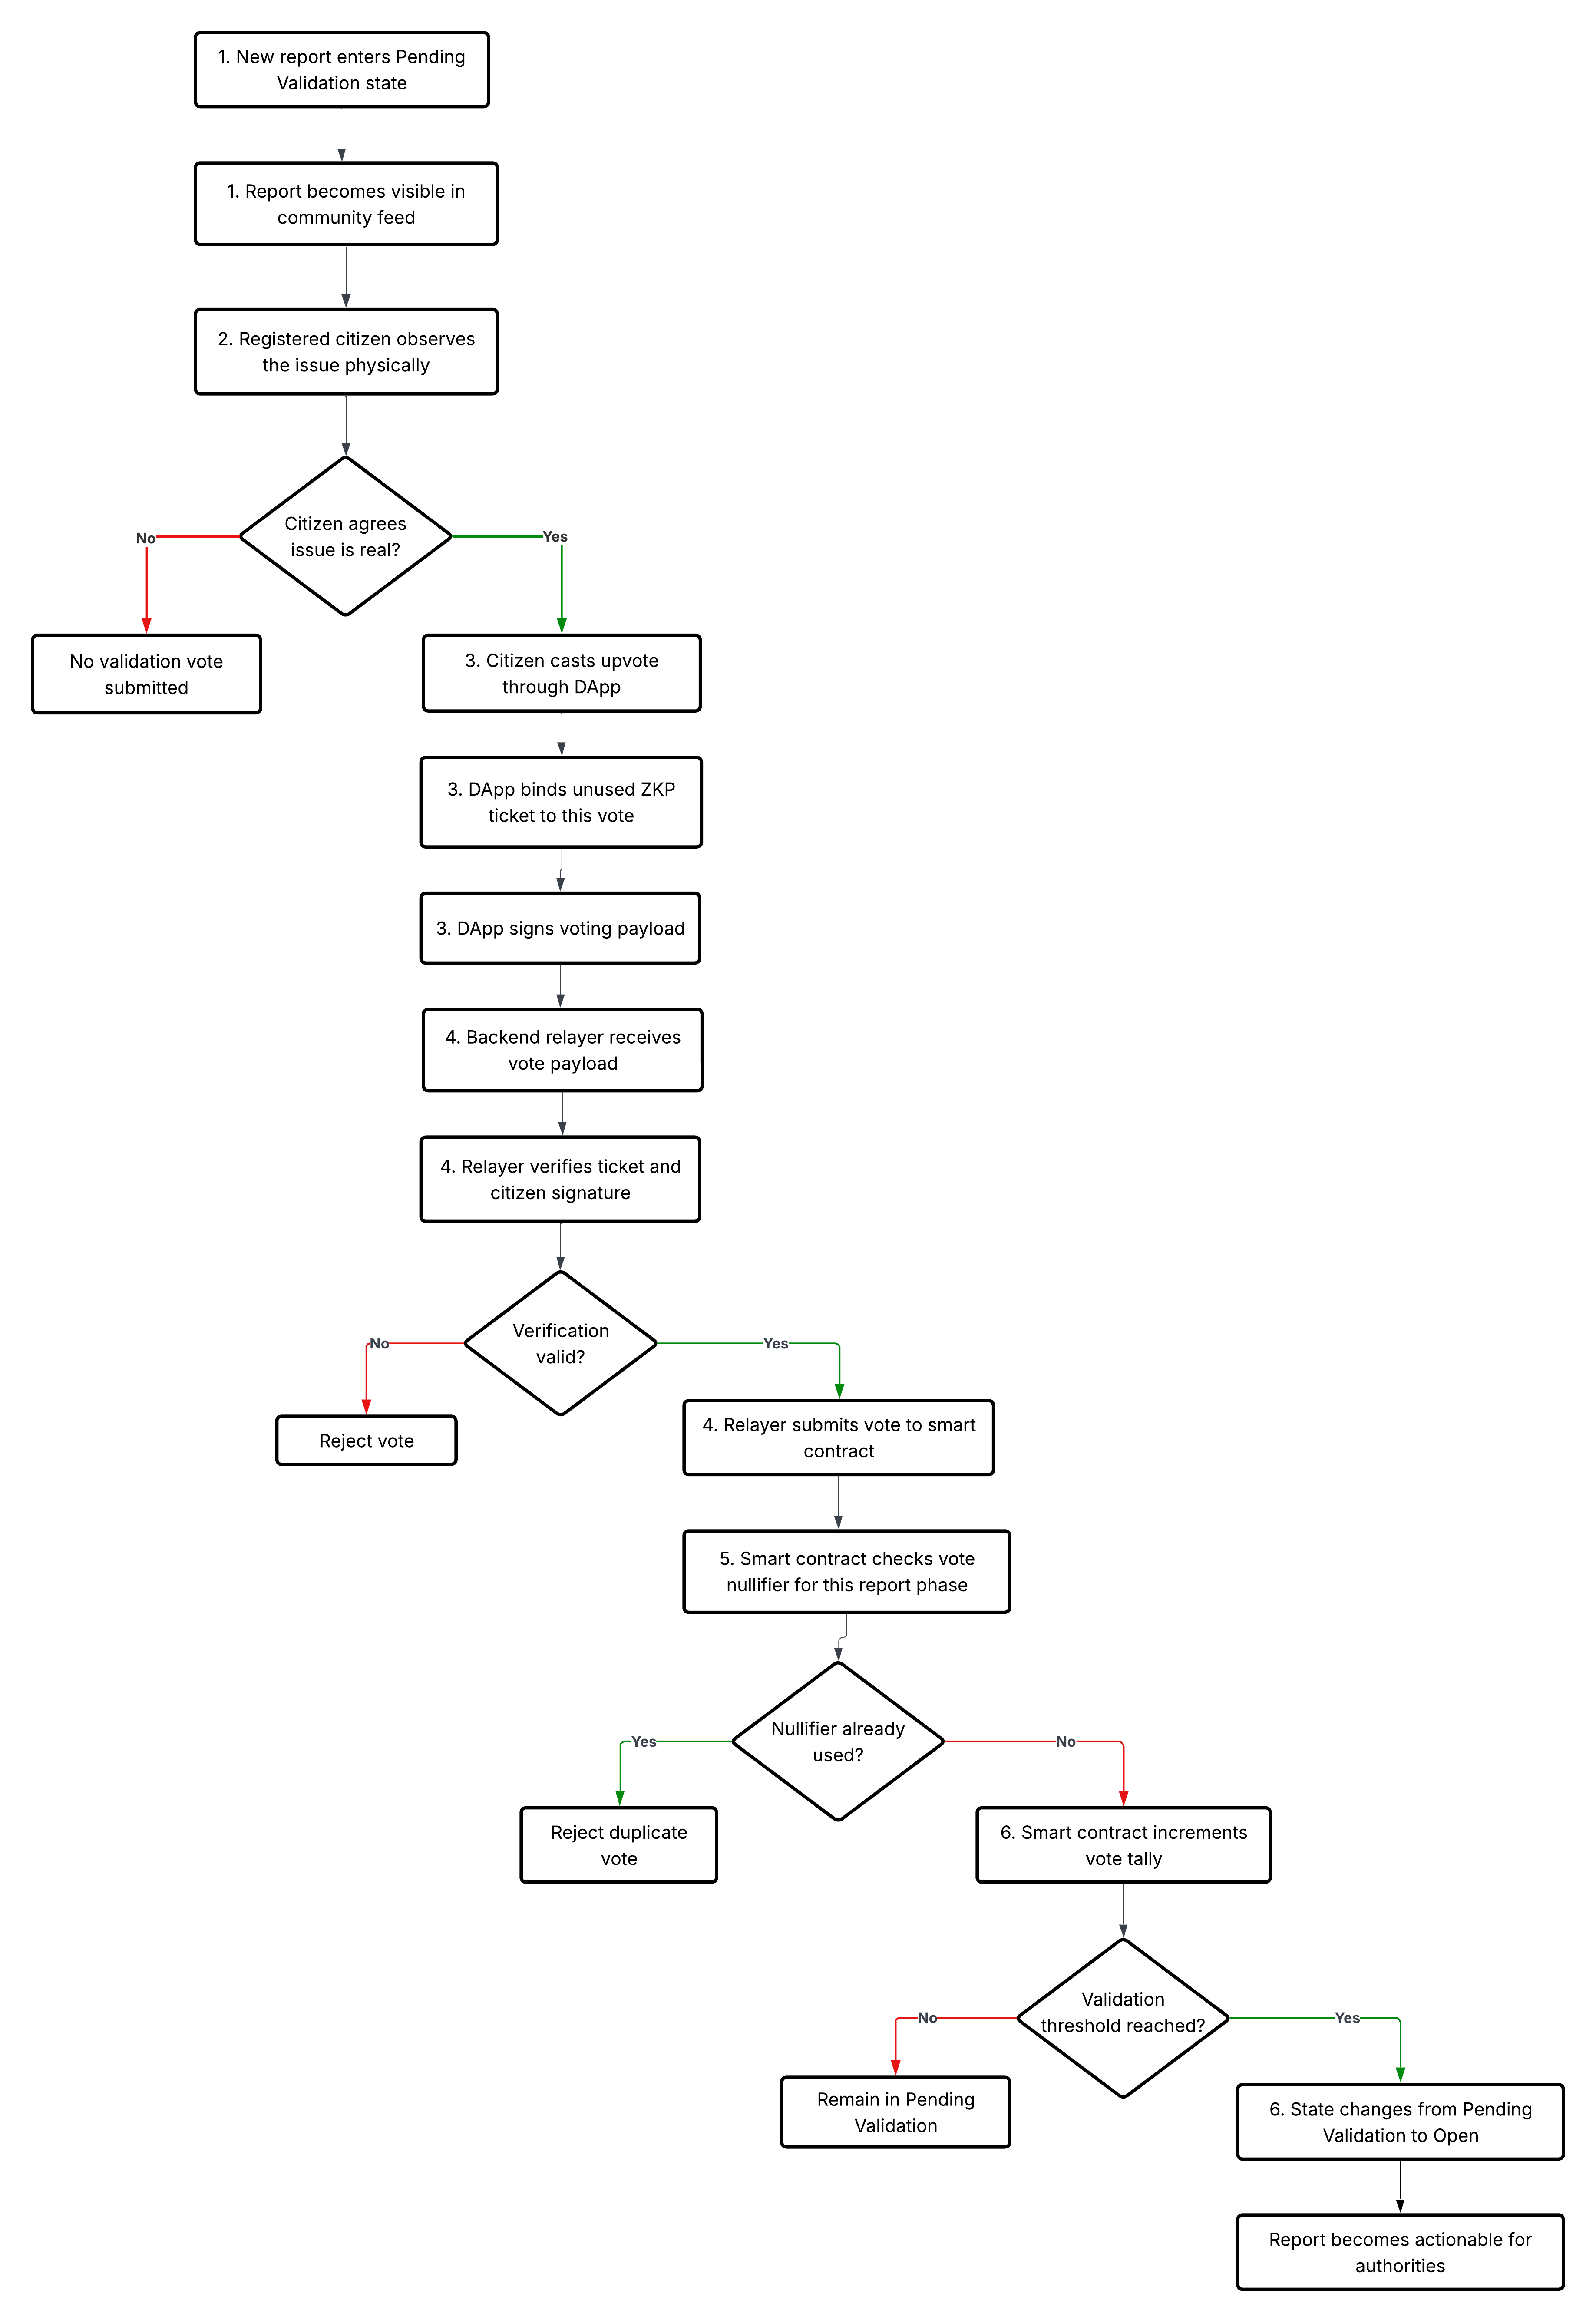
\includegraphics[width=0.95\textwidth,height=0.75\textheight,keepaspectratio]{Images/Chapter 3/community_validation_workflow.png}
    \caption{Community Consensus and Peer-Validation Workflow}
    \label{fig:community-validation-workflow}
\end{figure}

The validation workflow runs as follows:
\begin{enumerate}
    \item \textbf{Community Feed Display:} The public DApp feed shows reports in state $S_0$ with an active countdown timer indicating the 6-hour voting period.
    \item \textbf{Sybil-Resistant Vote Casting:} Citizens cast an upvote (\texttt{support = true}) or downvote (\texttt{support = false}) using an unused ticket nullifier.
    \item \textbf{Relayer Validation:} The relayer verifies the citizen's vote payload and submits the transaction to \texttt{castValidationVote} on \texttt{Reporting.sol}.
    \item \textbf{On-Chain Vote Tallying:} The smart contract checks that the vote nullifier has not been used before, records it, and increments either \texttt{validationUpvotes} or \texttt{validationDownvotes}.
    \item \textbf{State Finalization:} Finalization happens through two mechanisms:
    \begin{itemize}
        \item \textit{Lazy Evaluation:} If a vote is cast after the deadline (\texttt{block.timestamp > phaseDeadline}), the contract automatically calls \texttt{\_finalizeSingleReport}.
        \item \textit{Cron Finalization:} If no vote activity occurs, the \texttt{CronService} calls \texttt{batchFinalizeVotingWindows} daily at midnight.
    \end{itemize}
    If \texttt{upvotes > downvotes}, the report moves to $S_2$ (\texttt{Open}). Otherwise, it moves to $S_1$ (\texttt{CommunityRejected}).
\end{enumerate}

\subsection{Authority Resolution and Action Workflow}
\label{subsec:authority-workflow}

Reports that reach community consensus ($S_2 = \texttt{Open}$) are actionable for municipal authorities. Figure~\ref{fig:authority-action-workflow} shows the authority resolution workflow.

\begin{figure}[!htbp]
    \centering
    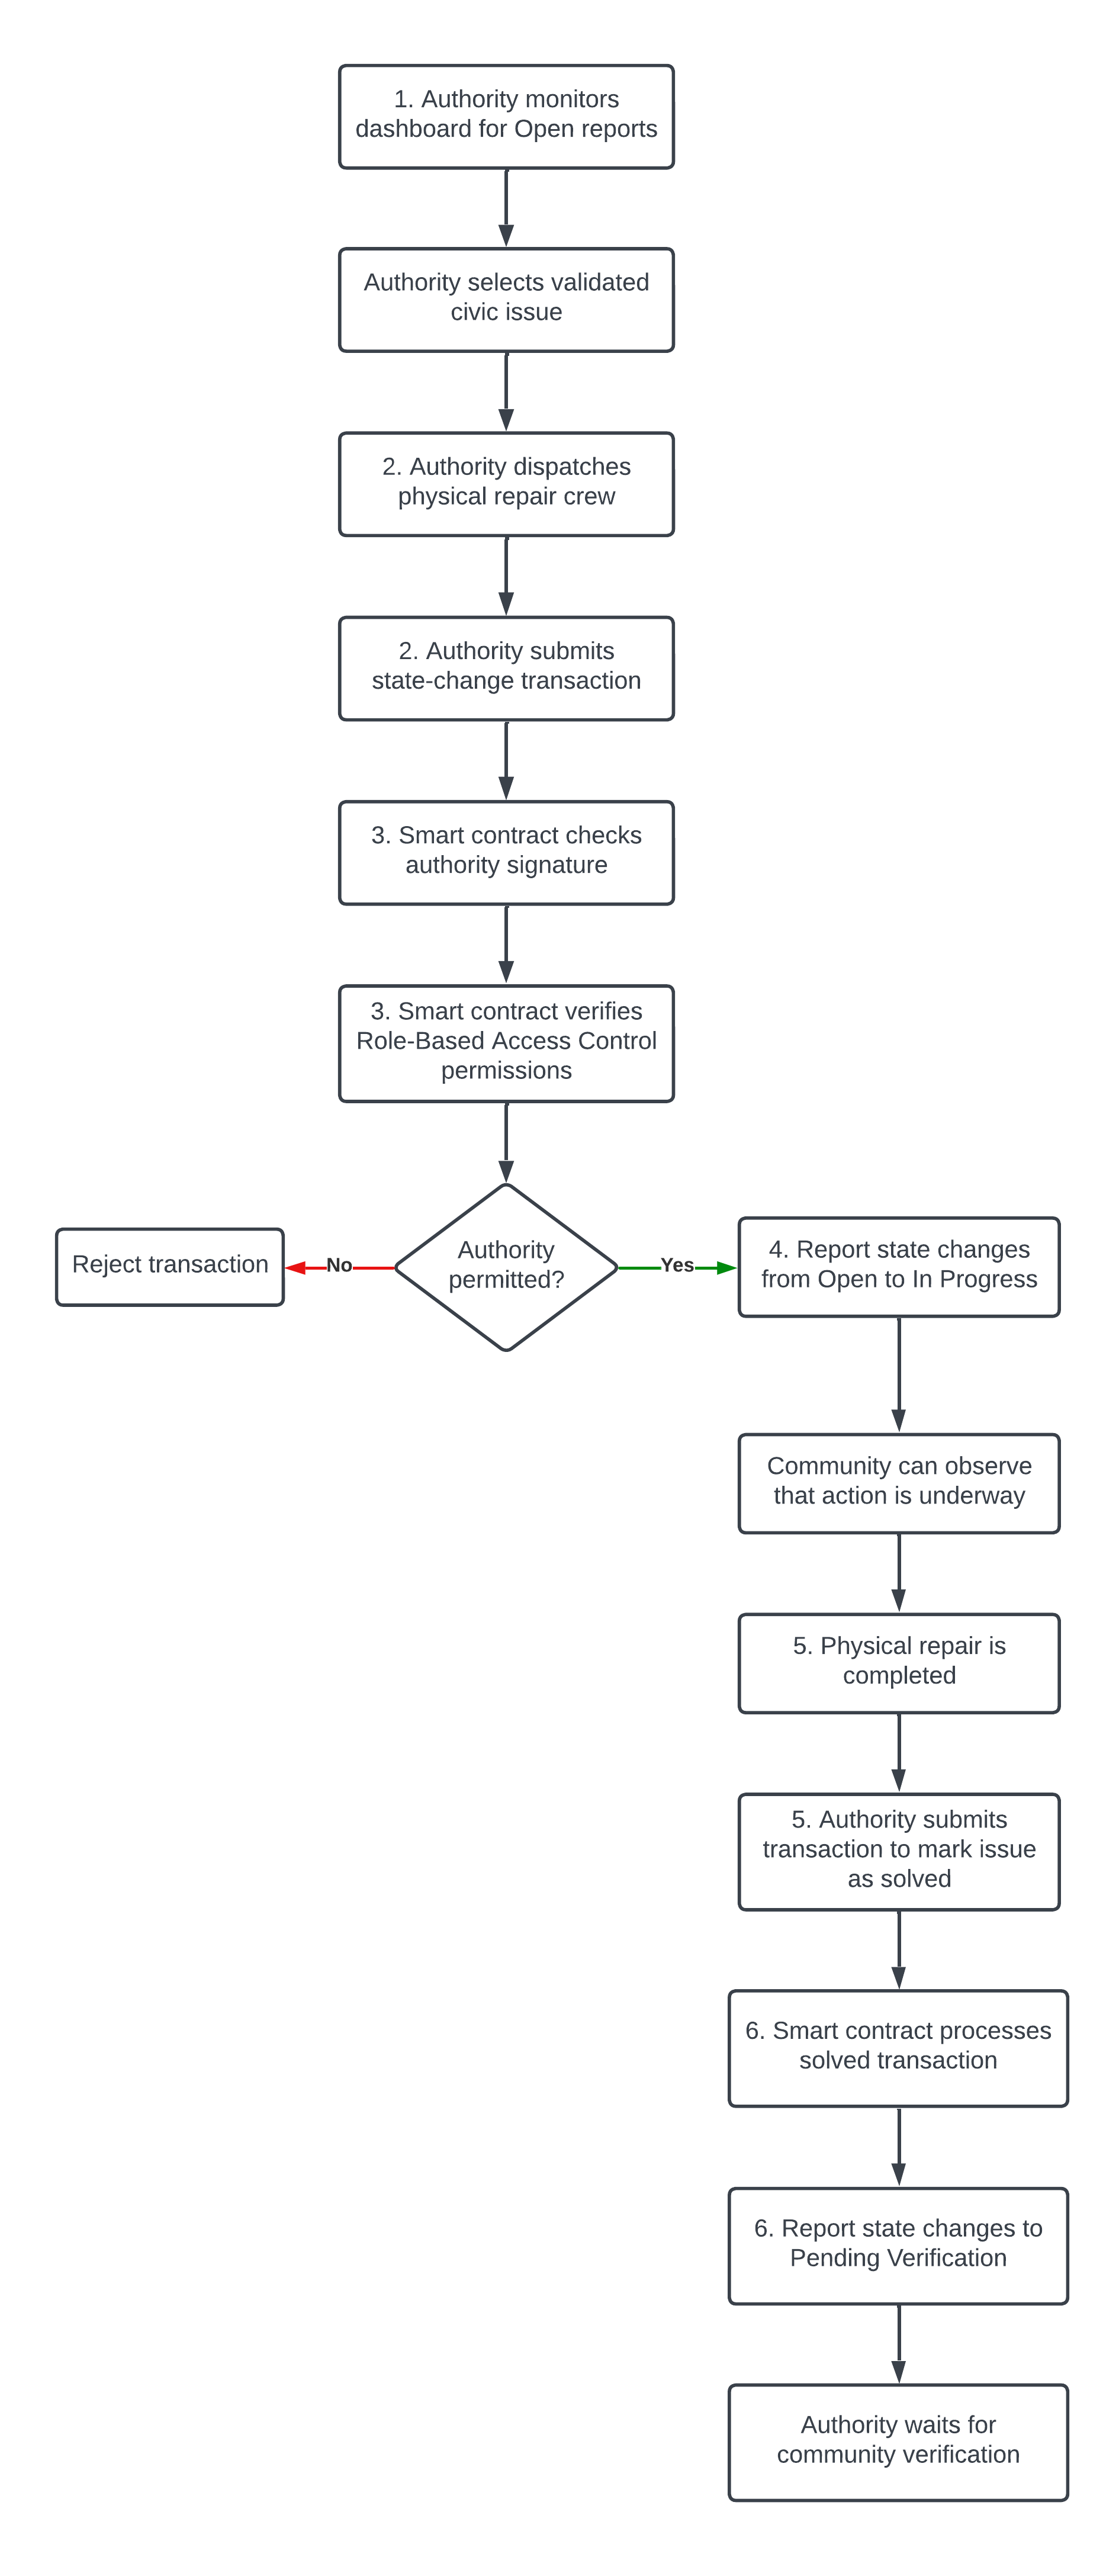
\includegraphics[width=0.95\textwidth,height=0.75\textheight,keepaspectratio]{Images/Chapter 3/authority_action_workflow.png}
    \caption{Authority Resolution and Infrastructure Repair Workflow}
    \label{fig:authority-action-workflow}
\end{figure}

The authority workflow has four operations:
\begin{enumerate}
    \item \textbf{Dashboard Monitoring:} Authorized municipal officials monitor validated reports through the authenticated Authority Dashboard. When an authority interacts with a report, their on-chain identity profile (name, position, department) is shown to the community.
    \item \textbf{Work Initiation (\texttt{startWork}):} An authority calls \texttt{startWork(reportId, comment, imageCid)} to claim an open issue. The smart contract verifies the caller is in \texttt{authorizedAuthorities}, sets \texttt{report.assignedAuthority}, changes the status to $S_3$ (\texttt{InProgress}), appends an \texttt{AuthorityAction} entry to the audit log, and emits \texttt{WorkStarted}.
    \item \textbf{Progress Updates (\texttt{addAuthorityUpdate}):} The assigned authority can post mid-repair updates using \texttt{addAuthorityUpdate}. This appends comments and progress image CIDs to the audit history without changing the report state.
    \item \textbf{Resolution Declaration (\texttt{markAsSolved}):} On completing repairs, the authority calls \texttt{markAsSolved(reportId, comment, imageCid)}, attaching photographic evidence. The contract transitions the report to $S_5$ (\texttt{PendingVerification}) and opens a 6-hour community verification window.
    \item \textbf{Issue Rejection (\texttt{rejectIssue}):} If a report is a duplicate, impossible to resolve, or outside the authority's jurisdiction, the authority calls \texttt{rejectIssue}. The contract changes the status to $S_4$ (\texttt{PendingRejectionReview}) and opens a 6-hour community appeal period.
\end{enumerate}

\subsection{Post-Resolution Verification and Appeal Workflow}
\label{subsec:post-res-workflow}

The system prevents authorities from closing reports unilaterally. Citizens must confirm that repairs are complete. Figure~\ref{fig:post-resolution-verification-workflow} shows this workflow.

\begin{figure}[!htbp]
    \centering
    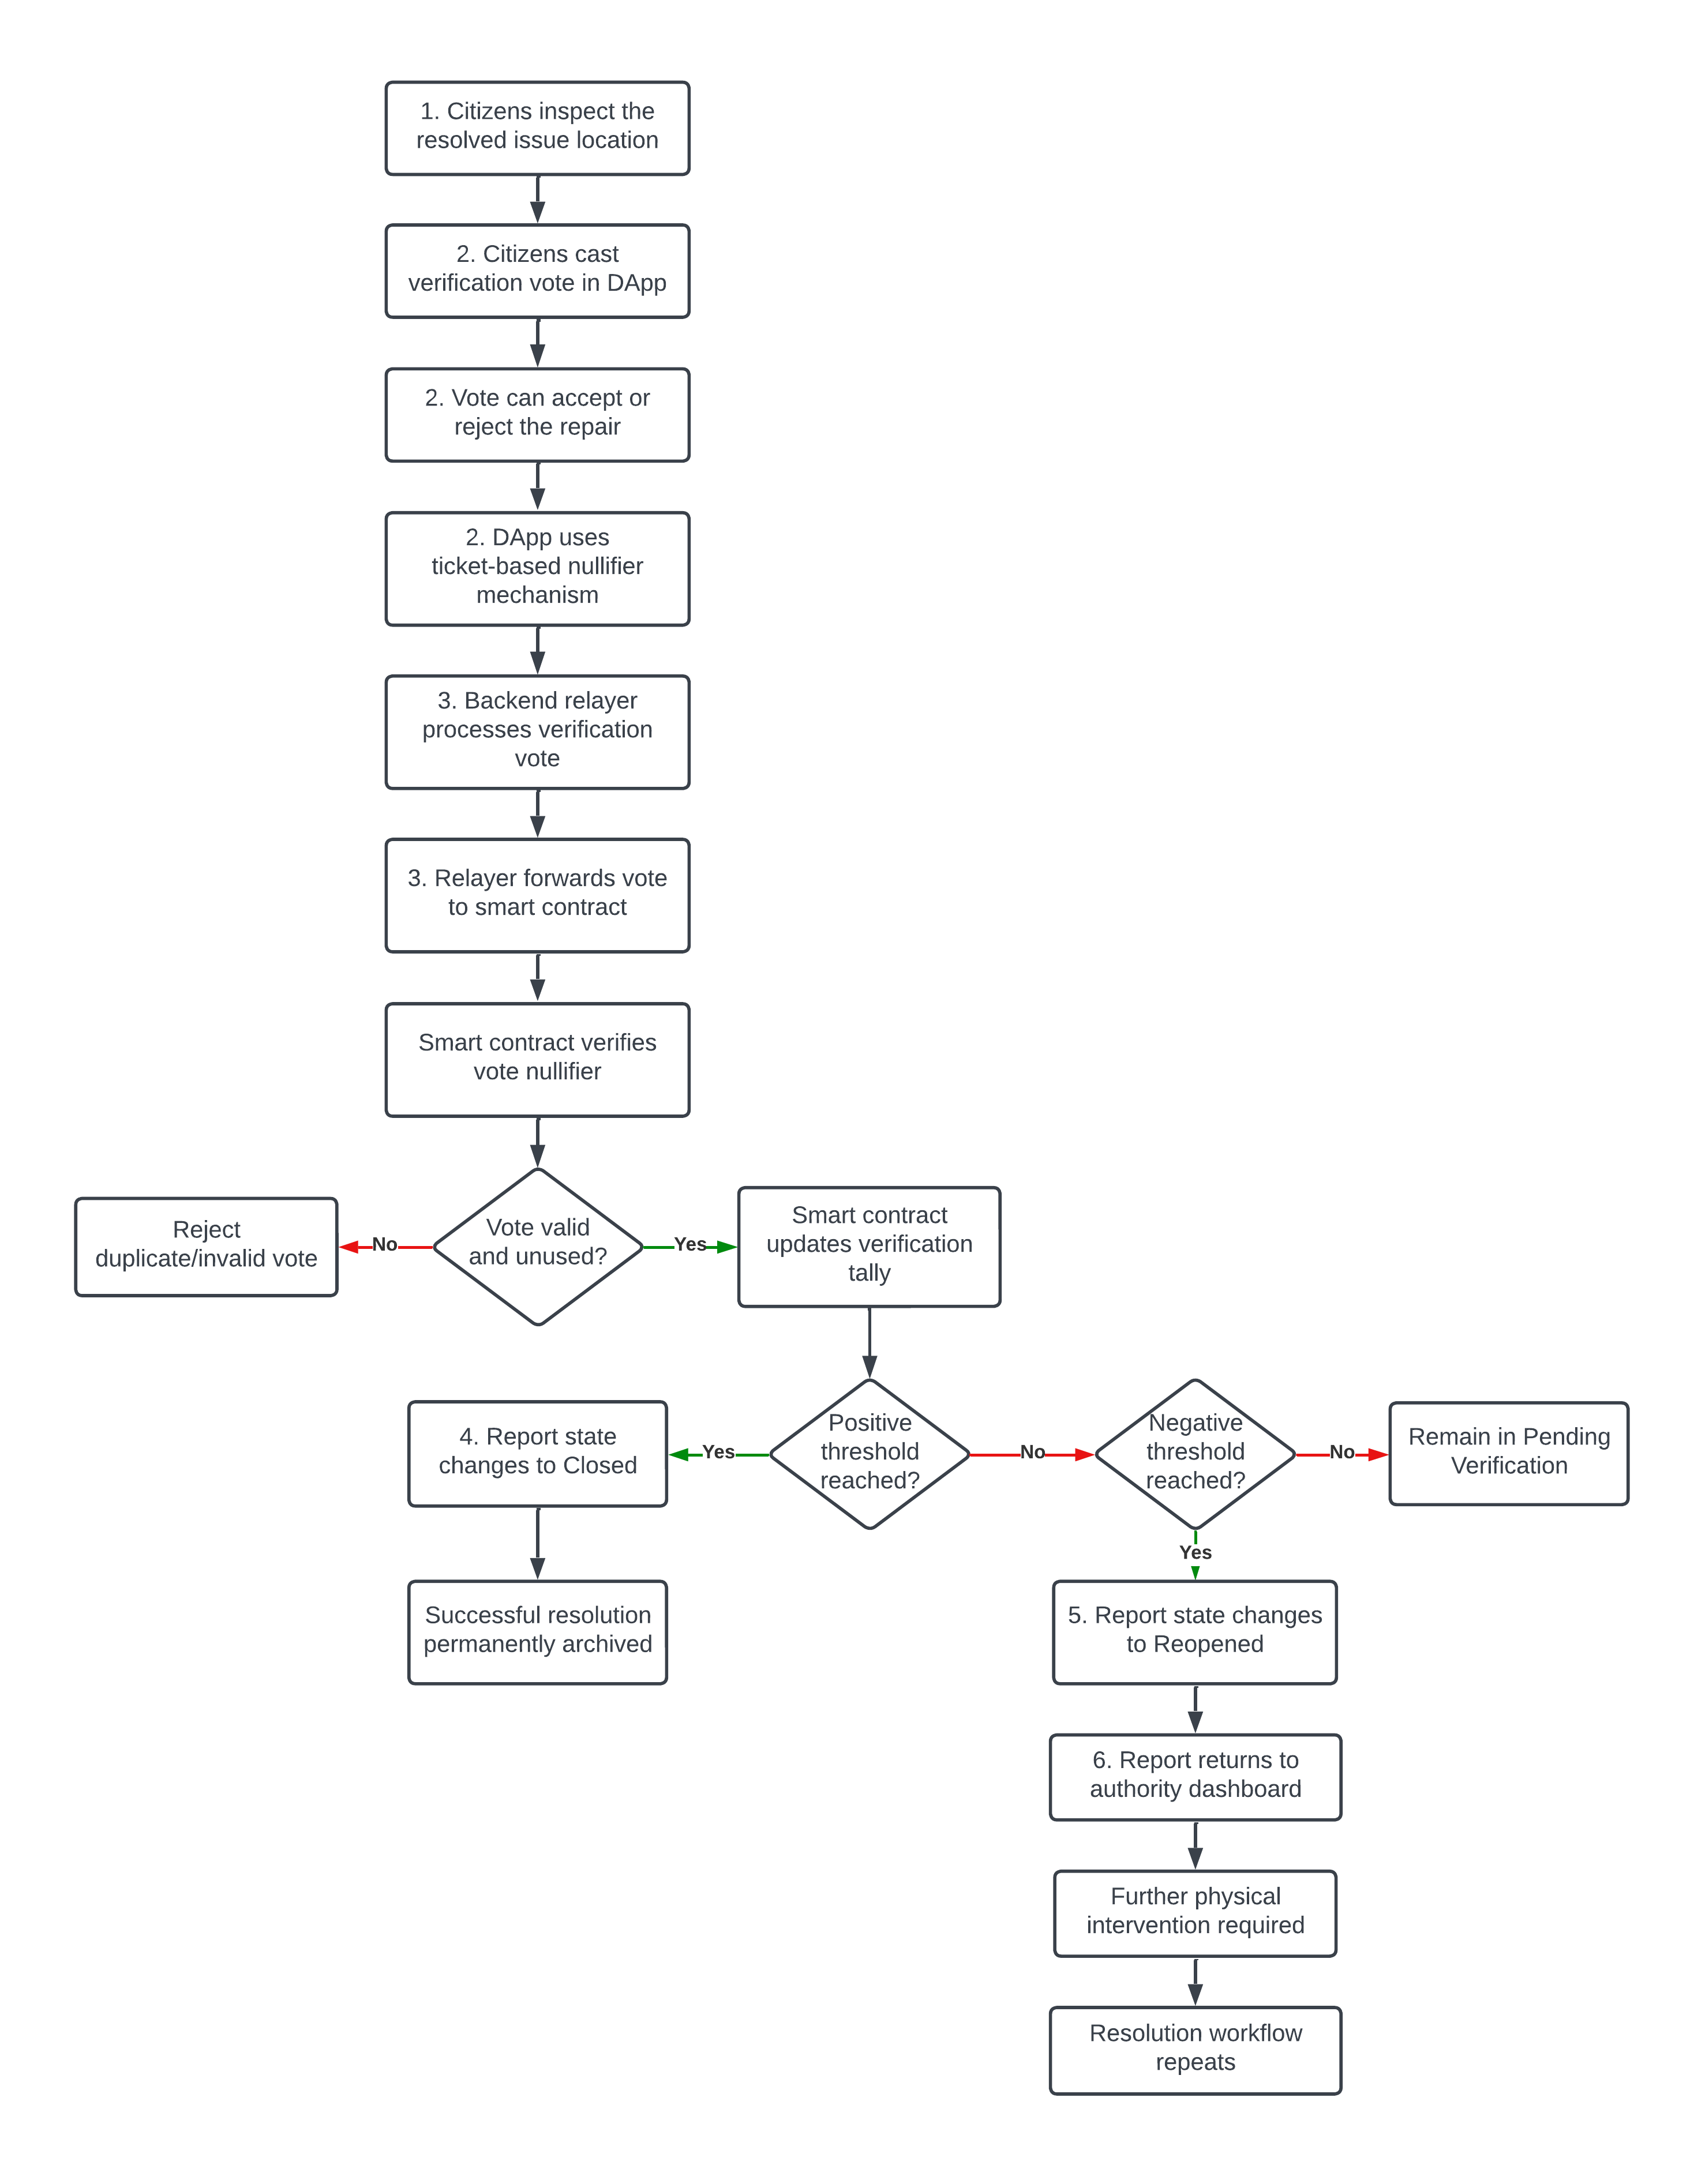
\includegraphics[width=0.95\textwidth,height=0.75\textheight,keepaspectratio]{Images/Chapter 3/post_resolution_verification_workflow.png}
    \caption{Post-Resolution Verification and Community Appeal Workflow}
    \label{fig:post-resolution-verification-workflow}
\end{figure}

Two review paths are defined:
\begin{enumerate}
    \item \textbf{Repair Verification ($S_5 = \texttt{PendingVerification}$):} Citizens inspect the completed repair and cast accept or reject votes using \texttt{castVerificationVote} within the 6-hour window. When the deadline elapses:
    \begin{itemize}
        \item If accept votes $\geq$ reject votes ($\rho_{\text{accept}} \ge \rho_{\text{reject}}$), the report moves to $S_6$ (\texttt{Closed}).
        \item If reject votes $>$ accept votes ($\rho_{\text{reject}} > \rho_{\text{accept}}$), the report moves to $S_7$ (\texttt{Reopened}).
    \end{itemize}
    \item \textbf{Rejection Review and Appeal ($S_4 = \texttt{PendingRejectionReview}$):} Citizens vote to uphold or appeal the authority rejection using \texttt{castRejectionReviewVote}. When the deadline elapses:
    \begin{itemize}
        \item If uphold votes $\geq$ appeal votes ($\upsilon_{\text{uphold}} \ge \upsilon_{\text{appeal}}$), the rejection is confirmed and the report moves to $S_6$ (\texttt{Closed}).
        \item If appeal votes $>$ uphold votes ($\upsilon_{\text{appeal}} > \upsilon_{\text{uphold}}$), the community appeal succeeds and the report moves to $S_7$ (\texttt{Reopened}).
    \end{itemize}
\end{enumerate}

\subsection{Anonymous Public Opinion Polling Workflow}
\label{subsec:opinion-polling-workflow}

The system also supports top-down municipal consultation through an anonymous public opinion polling workflow managed by \texttt{OpinionPolling.sol}. This allows local governments to collect democratic feedback on proposals such as public works, zoning changes, or budget allocations.

The opinion polling workflow has five steps:
\begin{enumerate}
    \item \textbf{Official Poll Creation:} An authorized municipal official calls \texttt{createOfficialPoll(ipfsMetadataCid, deadline, pollType)}, providing the IPFS CID of the proposal documentation, the deadline timestamp, and the poll type (\texttt{TrueFalse} or \texttt{MultiChoice}). The contract verifies the official's credentials, assigns a unique \texttt{pollId}, and emits \texttt{PollCreated}.
    \item \textbf{DApp Poll Display:} The DApp shows the voting options and proposal details retrieved from IPFS.
    \item \textbf{Anonymous Ballot Casting:} The citizen selects an option, signs the vote with an unused ticket nullifier, and the relayer submits the transaction to \texttt{castVote(pollId, optionIndex, nullifier)}.
    \item \textbf{Sybil-Resistant Tallying:} The smart contract checks that \texttt{nullifierVoted[pollId][nullifier]} is false, records the nullifier, and increments \texttt{pollResults[pollId][optionIndex]}.
    \item \textbf{Poll Finalization:} When the deadline elapses, any user or relayer can call \texttt{finalizePoll(pollId)}, marking the poll inactive and freezing the results.
\end{enumerate}

\section{Summary and Expected Outcomes}
\label{sec:summary-outcomes}

This chapter describes the system architecture, the six-layer topology, the subsystem communication protocols, the two-tier multi-signature governance model, and the operational workflows of the decentralised local governance reporting framework.

The expected outcomes of the architectural design are:
\begin{enumerate}
    \item \textbf{Citizen Anonymity and Privacy:} Zero-knowledge authentication and single-use ticket nullifiers fully separate real-world citizen identity from on-chain actions.
    \item \textbf{Decentralized Municipal Governance:} \texttt{AuthorityMultiSig.sol} ensures that access to authority and identity profiles is controlled by a majority quorum of Super Admins.
    \item \textbf{Automated Off-Chain Orchestration:} The \texttt{AuthorityFundingService} and \texttt{CronService} remove the need for manual treasury management and ensure deterministic finalization of expired voting windows.
    \item \textbf{Tamper-Evident Accountability:} Report metadata, state transitions, authority action logs, and voting tallies are stored on-chain as an immutable audit trail.
    \item \textbf{Automated Spam and Toxicity Mitigation:} The multi-oracle AI Moderation Ensemble prevents abusive, irrelevant, or malicious content from entering the system.
    \item \textbf{Democratic Lifecycle Oversight:} Sybil-resistant community voting at the validation, verification, and appeal stages prevents arbitrary dismissal of reports and ensures repair quality.
    \item \textbf{High Usability and Gasless Interaction:} The relayer pattern eliminates cryptocurrency onboarding barriers. Citizens interact through a standard web application.
\end{enumerate}

With the system architecture, mathematical state machine, governance topology, and workflows fully specified, Chapter 4 presents the technical implementation of each architectural component.


% \chapter{System Architecture and Workflow Design}
% \label{ch:architecture}

% The chapter sets out the complete architectural framework and the design of the operational workflow for the proposed blockchain-based, community-assisted, privacy-preserving reporting platform concerning local governance. To attain an optimal balance between citizen anonymity, data immutability, spam prevention, transparent civic accountability, and decentralised administrative governance, a well-structured, multi-layered system architecture is required. In this chapter the allocation of responsibilities between the on-chain and off-chain components is explained, the communication and verification procedures between the various layers of the architecture are specified, the mathematical and finite state machine (Finite State Machine (\ac{FSM})) models that control the lifecycle of issues are defined, and the deterministic workflows carried out during citizen authentication, report submission, community validation, authority resolution, public opinion polling, and two-tier multi-signature governance are outlined.

% \section{Overall System Architecture}
% \label{sec:overall-architecture}

% The system in question makes use of a combined on-chain and off-chain architectural approach. Although decentralized ledger technology ensures immutability, transparency, and the presence of tamper-evident audit trails, it is technically impossible and economically unreasonable to carry out high-capacity media storage and the execution of computationally complex algorithms directly on the chain. As a result, the architecture fully separates the management of the immutable state and cryptographic verification from the storage of data and the evaluation of content.

% \subsection{Hybrid On-Chain/Off-Chain Model}
% \label{subsec:hybrid-model}

% The hybrid model separates system operations into two synchronized environments:
% \begin{enumerate}
%     \item \textbf{On-Chain Execution Environment:} The on-chain execution environment has been implemented as a private and permissioned PoA blockchain network. It holds only minimal and immutable state information, such as report metadata, the various lifecycle state transitions, the cryptographic hashes of the report payloads, the one-time ticket nullifiers, the role-based access control (\ac{RBAC}) permissions, the two-tier multi-signature governance proposals, the on-chain official identity profiles, and the results of community voting.
%     \item \textbf{Off-Chain Execution Environment:} This refers to the set of computationally demanding and data-intensive operations which cannot take place on-chain, such as storing high-resolution multimedia evidence in \ac{IPFS}, carrying out automated natural language and visual content moderation using an ensemble of \ac{AI} classifiers, carrying out gasless transaction orchestration through a middleware backend relayer, providing automated account funding by means of event listeners, and carrying out background cron jobs for the batch finalisation of voting windows.
% \end{enumerate}

% Figure~\ref{fig:overall-architecture} shows the high-level architecture of the system, indicating the structural boundaries and the data links between the user interface, the identity verification layer, the middleware orchestrator, the off-chain services, and the permissioned blockchain ledger.

% \begin{figure}[!htbp]
%     \centering
%     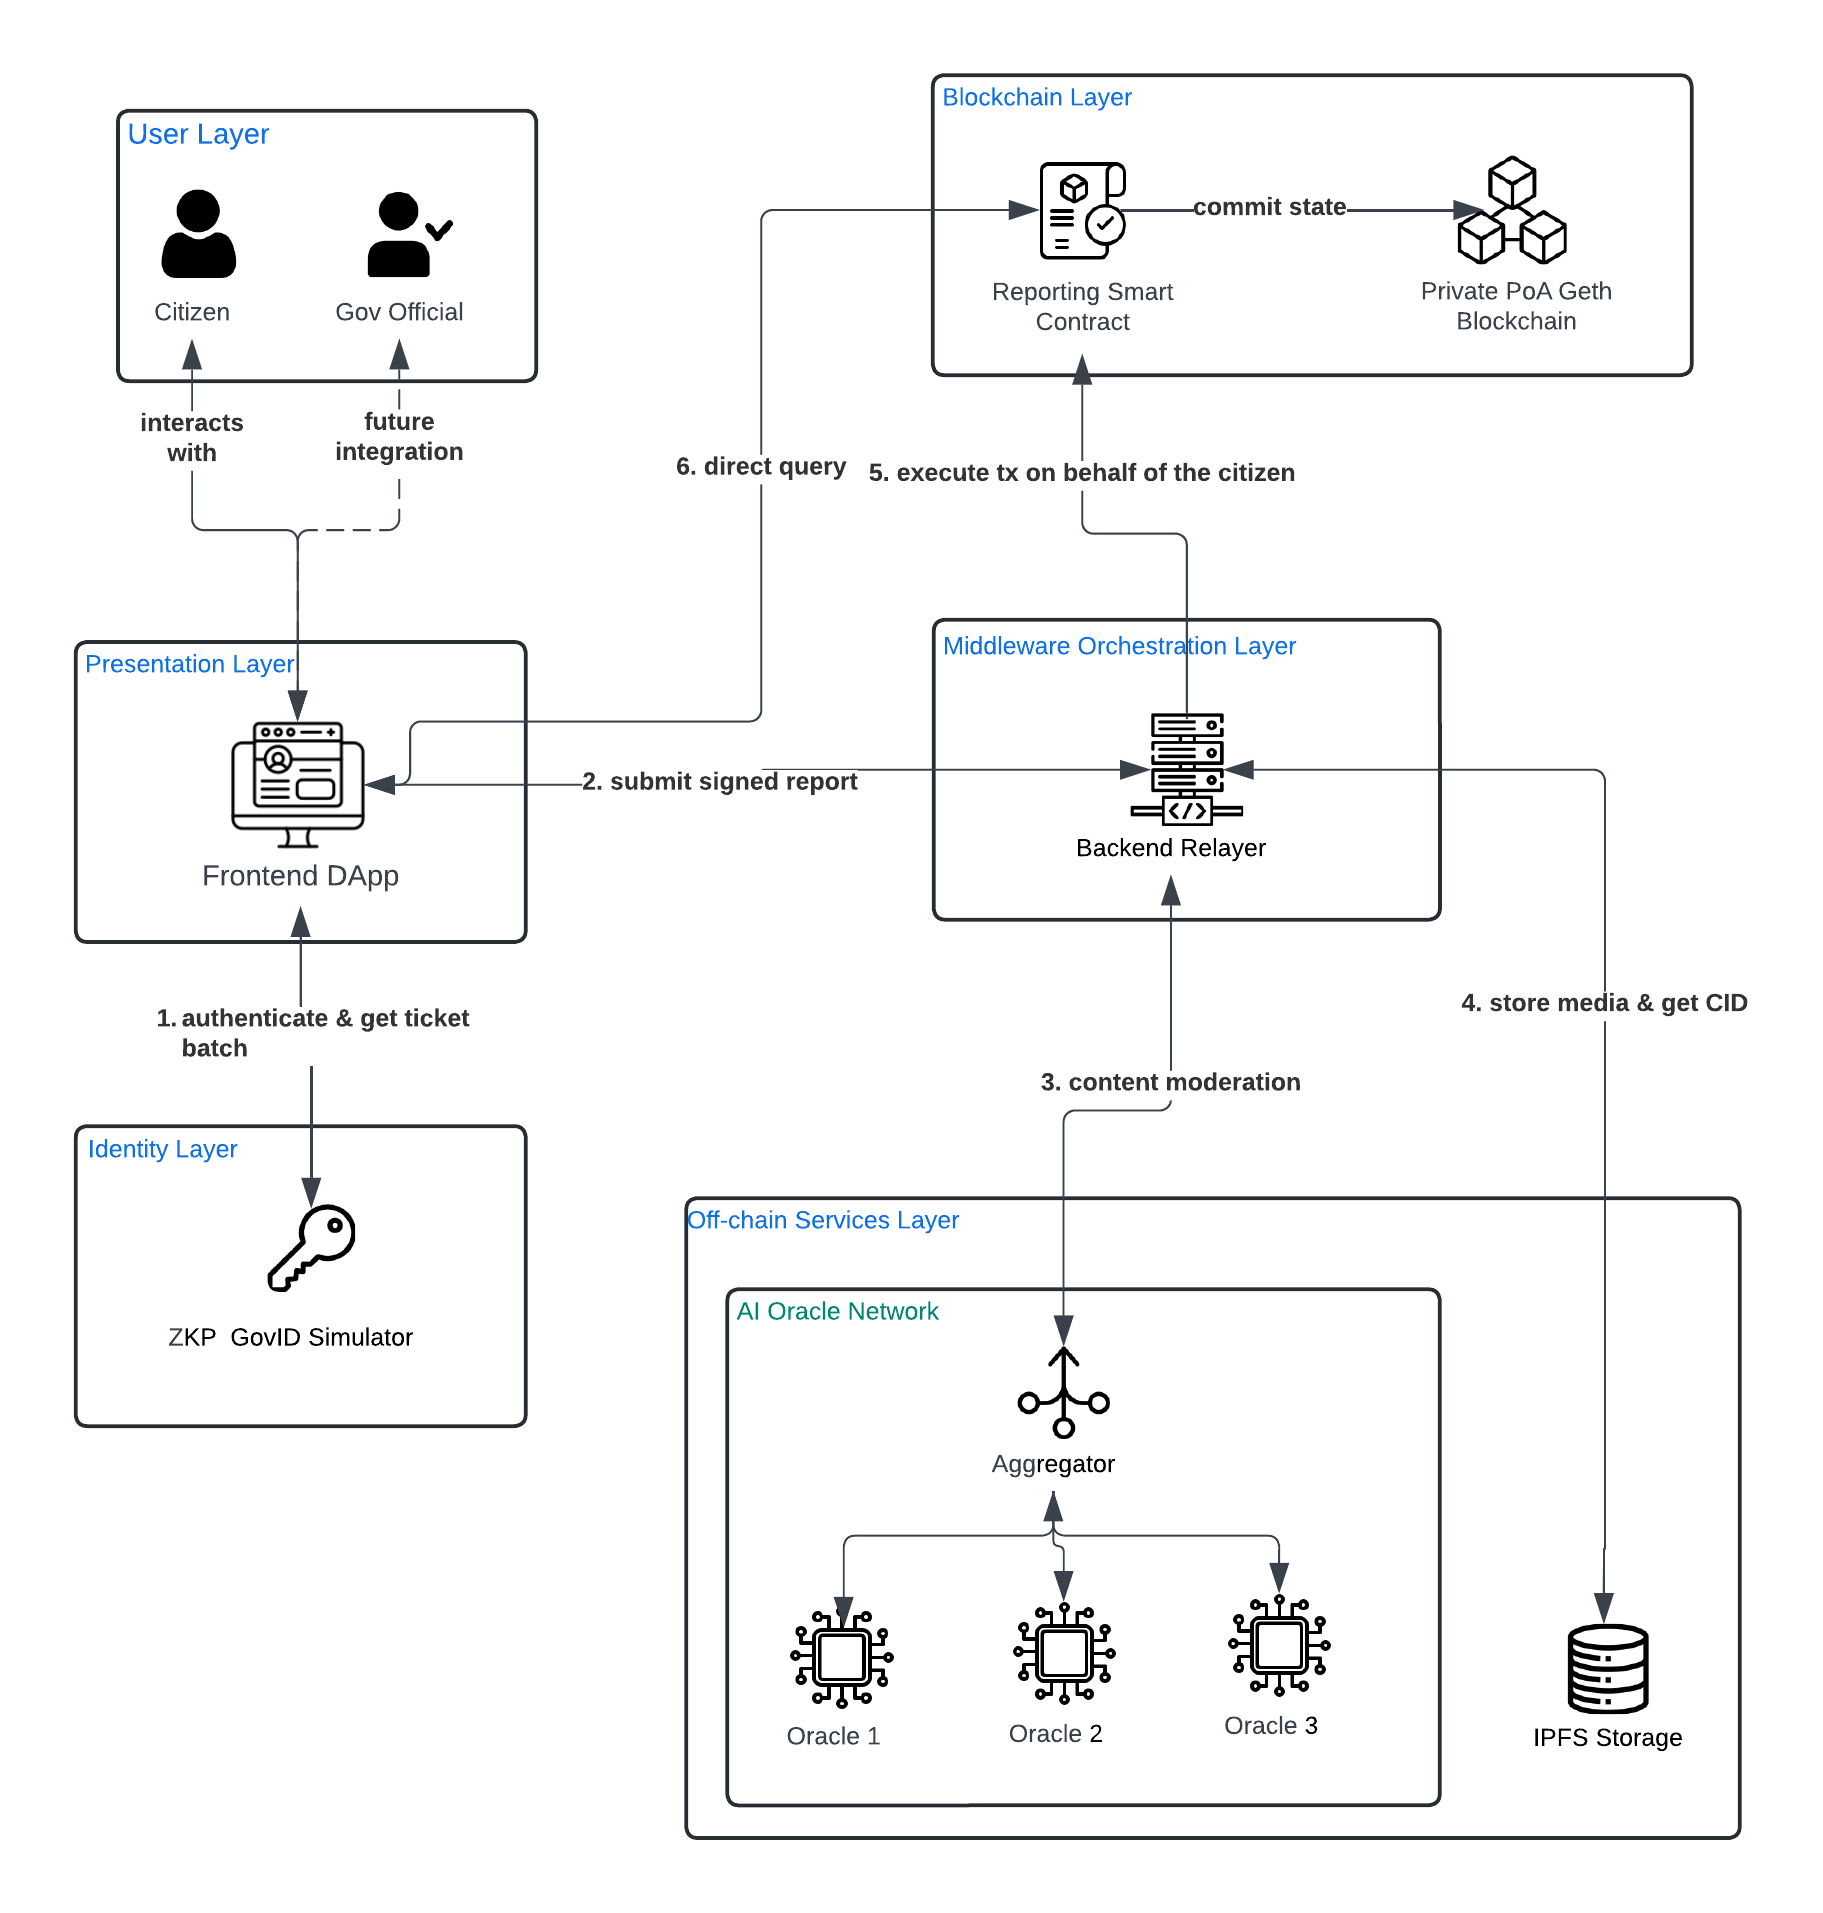
\includegraphics[width=0.95\textwidth,height=0.75\textheight,keepaspectratio]{Images/Chapter_3/overall-architecture.png}
%     \caption{High-Level Architectural Diagram of the Proposed System}
%     \label{fig:overall-architecture}
% \end{figure}

% The system is able to maintain the confidentiality of citizen identities while at the same time ensuring that all the reports submitted, the voting actions, the responses from authorities, and the assignments of administrative roles remain publicly verifiable and are resistant to unilateral alteration or censorship.

% \subsection{Six-Layer Architectural Topology}
% \label{subsec:six-layer-topology}

% In order to attain modularity, fault isolation, and scalability, the entire architecture is divided into a six-layer structure, each layer taking on specific functional responsibilities and providing standard interfaces to the layers next to it:

% \begin{enumerate}
%     \item \textbf{User Layer:}

%     This layer includes the main actors who interact with the ecosystem, namely ordinary citizens, the authorities of the municipal government, and previously approved institutional stakeholders such as Non-Governmental Organisations \ac{NGO}. Citizens submit reports about civic issues and take part in validation voting, while the authorities keep an eye on the matter, claim the reported infrastructure problems and resolve them all under the oversight of the municipal Super Admins.


%     \item \textbf{Presentation (DApp) Layer:}

%     The presentation layer is a responsive, web-based \ac{DApp} developed using Next.js and React, and it functions as the main interface for citizens, government officials, and municipal administrators. Citizens are offered intuitive workflows which allow them to carry out authentication, submit reports, upload media, browse the community feed, and vote anonymously. For authorities and Super Admins, the layer provides an authenticated dashboard which enables them to keep track of open reports, claim tasks, post mid-work progress updates, mark issues as resolved, and either submit or vote on two-tier multi-signature governance proposals. This presentation layer hides the underlying blockchain complexity so that users do not need to install cryptocurrency wallets or deal with native gas assets.


%     \item \textbf{Identity and Authentication Layer:}
%     This layer has the function of verifying the credentials of citizens and providing cryptographic proof of their entitlements without linking any personal identifiable information to the on-chain activities. It is achieved through the use of the Zero-Knowledge Proof (\ac{ZKP}) GovID Simulator, which authenticates citizens against an official municipal registry and produces batches of single-use ticket identifiers (\texttt{zkpTicketId}) that are signed by the government together with a unique citizen seed. This approach sets up a trust anchor that stops Sybil attacks while at the same time ensuring full identity decoupling.

%     \item \textbf{Middleware Orchestration (Relayer) Layer:}
%     The backend relayer acts as the centralized gateway and coordination bridge between web clients and the blockchain network. Built using NestJS, the relayer receives signed report payloads and meta-transactions from the \ac{DApp}, executes a dual-layer cryptographic verification of government-signed tickets and citizen signatures, forwards report text and media to the \ac{AI} moderation service, anchors accepted content to \ac{IPFS}, and submits gas-sponsored transactions to the blockchain on behalf of users. Additionally, this layer incorporates an automated \texttt{AuthorityFundingService} to fund newly approved municipal workers and a background \texttt{CronService} to execute automated batch finalization of expired voting phases.

%     \item \textbf{Off-Chain Services Layer:}
%     This layer hosts specialized services required for content validation and decentralized storage:
%     \begin{itemize}
%         \item \textit{AI Content Moderation Ensemble:} A machine learning service using multiple oracles which assesses textual descriptions and visual evidence for spam, toxicity, abuse, and civic relevance prior to submission to the blockchain.
%         \item \textit{IPFS Distributed Storage:} A peer-to-peer storage network which keeps the original report descriptions, images, and completion evidence and returns immutable \ac{CID} that are then recorded on the blockchain.
%     \end{itemize}

%     \item \textbf{Blockchain Ledger Layer:}
%     The foundation of the architecture is a private, permissioned blockchain running under the Clique \ac{PoA} consensus engine. This layer executes the compiled smart contract suite—comprising \texttt{Reporting.sol}, \texttt{OpinionPolling.sol}, and \texttt{AuthorityMultiSig.sol}—which enforce deterministic lifecycle rules, manage two-tier municipal access control, maintain on-chain profile directories, track one-time ticket nullifiers, and record an append-only audit trail of all governance events

% \end{enumerate}

% \section{Subsystem Interconnection \& Interaction Design}
% \label{sec:subsystem-interconnection}

% The operational integrity of the platform depends on robust, cryptographically secure communication protocols between the six architectural layers. This section details the interface specifications, verification mechanisms, decentralized governance topology, automated funding services, and interconnection topologies that bind the subsystems together.

% \subsection{Communication Protocols and Interface Specifications}
% \label{subsec:comm-protocols}

% Inter-layer communication is governed by three primary protocol interfaces:
% \begin{enumerate}
%     \item \textbf{REST/HTTPS API Protocols:} For the REST/HTTPS API protocols, the \ac{DApp} sends its communications to both the ZKP GovID Simulator and the Backend Relayer via secure HTTPS. When it submits reports, requests tickets, or carries out polling queries, it does so by using standard JSON payloads. The REST endpoints include rate-limiting, request validation, and transport-layer encryption. 
%     \item \textbf{JSON-RPC and WebSocket Protocols:} For the backend relayer and \ac{AI} Oracle workers, communication with the private PoA blockchain takes place through Ethereum-compatible JSON-RPC and WebSocket connections using HTTP or WSS. The use of WebSocket providers allows for real-time event streaming, which enables the off-chain workers to subscribe to events such as \texttt{ReportCreated}, \texttt{ReportStatusChanged}, and \texttt{ProposalExecuted} with a latency of less than a second.
%     \item \textbf{IPFS HTTP Gateway and RPC API:} For pinning files and obtaining metadata, the Backend Relayer and \ac{AI} Oracles communicate with the local \ac{IPFS} daemon through its RPC API (on port 5001), whereas media rendering on the client side makes use of decentralised HTTP gateways.
% \end{enumerate}

% \subsection{Dual-Layer Cryptographic Verification Engine}
% \label{subsec:dual-layer-verification}

% In order not to require citizens to submit their transactions directly to the blockchain and at the same time to prevent unauthorized submissions and payload tampering, the Backend Relayer makes use of a dual-layer cryptographic verification engine. When a citizen submits a report, the relayer checks two separate signatures before carrying out off-chain storage or on-chain anchoring:

% \begin{enumerate}
%     \item \textbf{Government Ticket Authenticity Verification:} The relayer checks the single-use ticket identifier (\texttt{zkpTicketId}) included in the request and verifies the cryptographic signature that was generated by the ZKP GovID Simulator using the official government authority’s ECDSA public key; this ensures that the person making the submission is a verified citizen and that the ticket has not been forged.
%     \item \textbf{Citizen Payload Integrity Verification:} The relayer checks the ECDSA signature that the citizen has signed over the composite report hash, which is defined mathematically by the equation:
%     \begin{equation}
%         \mathcal{H}_{\text{report}} = \text{keccak256}\Big(\text{description} \parallel \text{zkpTicketId} \parallel \mathcal{H}_{\text{media}}\Big)
%     \end{equation}
%     The relayer is able to ensure that neither man-in-the-middle attackers nor the relayer itself have altered the report description or the media evidence because the payload hash signed by the citizen's ephemeral private key matches the data that has been received.
% \end{enumerate}

% Figure~\ref{fig:backend-relayer-impl} shows the internal architecture of the Backend Relayer, emphasizing the request validation pipeline, the signature verification engine, the gas sponsorship module, and the transaction dispatcher.

% \begin{figure}[!htbp]
%     \centering
%     \includegraphics[width=0.95\textwidth,height=0.75\textheight,keepaspectratio]{Images/Chapter 3/backend-relayer-impl.png}
%     \caption{Backend Relayer Middleware Implementation and Verification Pipeline}
%     \label{fig:backend-relayer-impl}
% \end{figure}

% \subsection{AI Moderation Oracle Ensemble Interconnection}
% \label{subsec:ai-oracle-interconnection}

% Content moderation is carried out by a network of machine learning oracles which are designed to filter out spam, harmful text, and non-civic material before the content is permanently anchored on-chain. This network consists of three specialized oracle nodes that are coordinated by an Oracle Aggregator.

% \begin{enumerate}
%     \item \textbf{Safety Oracle Node:} The Safety Oracle Node uses fine-tuned transformer models (specifically \texttt{unitary/toxic-bert}) to assess textual submissions for any abusive, hateful or threatening language and employs deep learning image classifiers to check visual material for inappropriate or adult content
%     \item \textbf{Spam and Abuse Oracle Node:} Unsolicited promotional messages, gibberish, and repetitive flood attacks are detected by means of lightweight classification models (\texttt{bert-tiny-finetuned-sms-spam-detection}) together with statistical heuristic filters
%     \item \textbf{Civic Relevance Oracle Node:} Using the \texttt{sentence-transformers/all-MiniLM-L6-v2} model it produces semantic vector embeddings of the report descriptions and calculates cosine similarity scores based on a domain-specific lexicon of municipal infrastructure categories (such as road hazards, sanitation, and street lighting) in order to reject irrelevant submissions
%     \item \textbf{Oracle Aggregator Node:} This functions as the central verification gateway. It gathers the signed moderation decisions from each oracle worker, checks the request nonces and timestamps in order to guard against replay attacks, enforces an immediate rejection override when the Safety Oracle identifies severe toxicity, and otherwise uses a majority-consensus rule to arrive at a final \texttt{ACCEPT} or \texttt{REJECT} decision
% \end{enumerate}

% Figure~\ref{fig:oracle-architecture} details the interconnection topology of the \ac{AI} Content Moderation Ensemble and its synchronization with the Backend Relayer and smart contract event stream.

% \begin{figure}[!htbp]
%     \centering
%     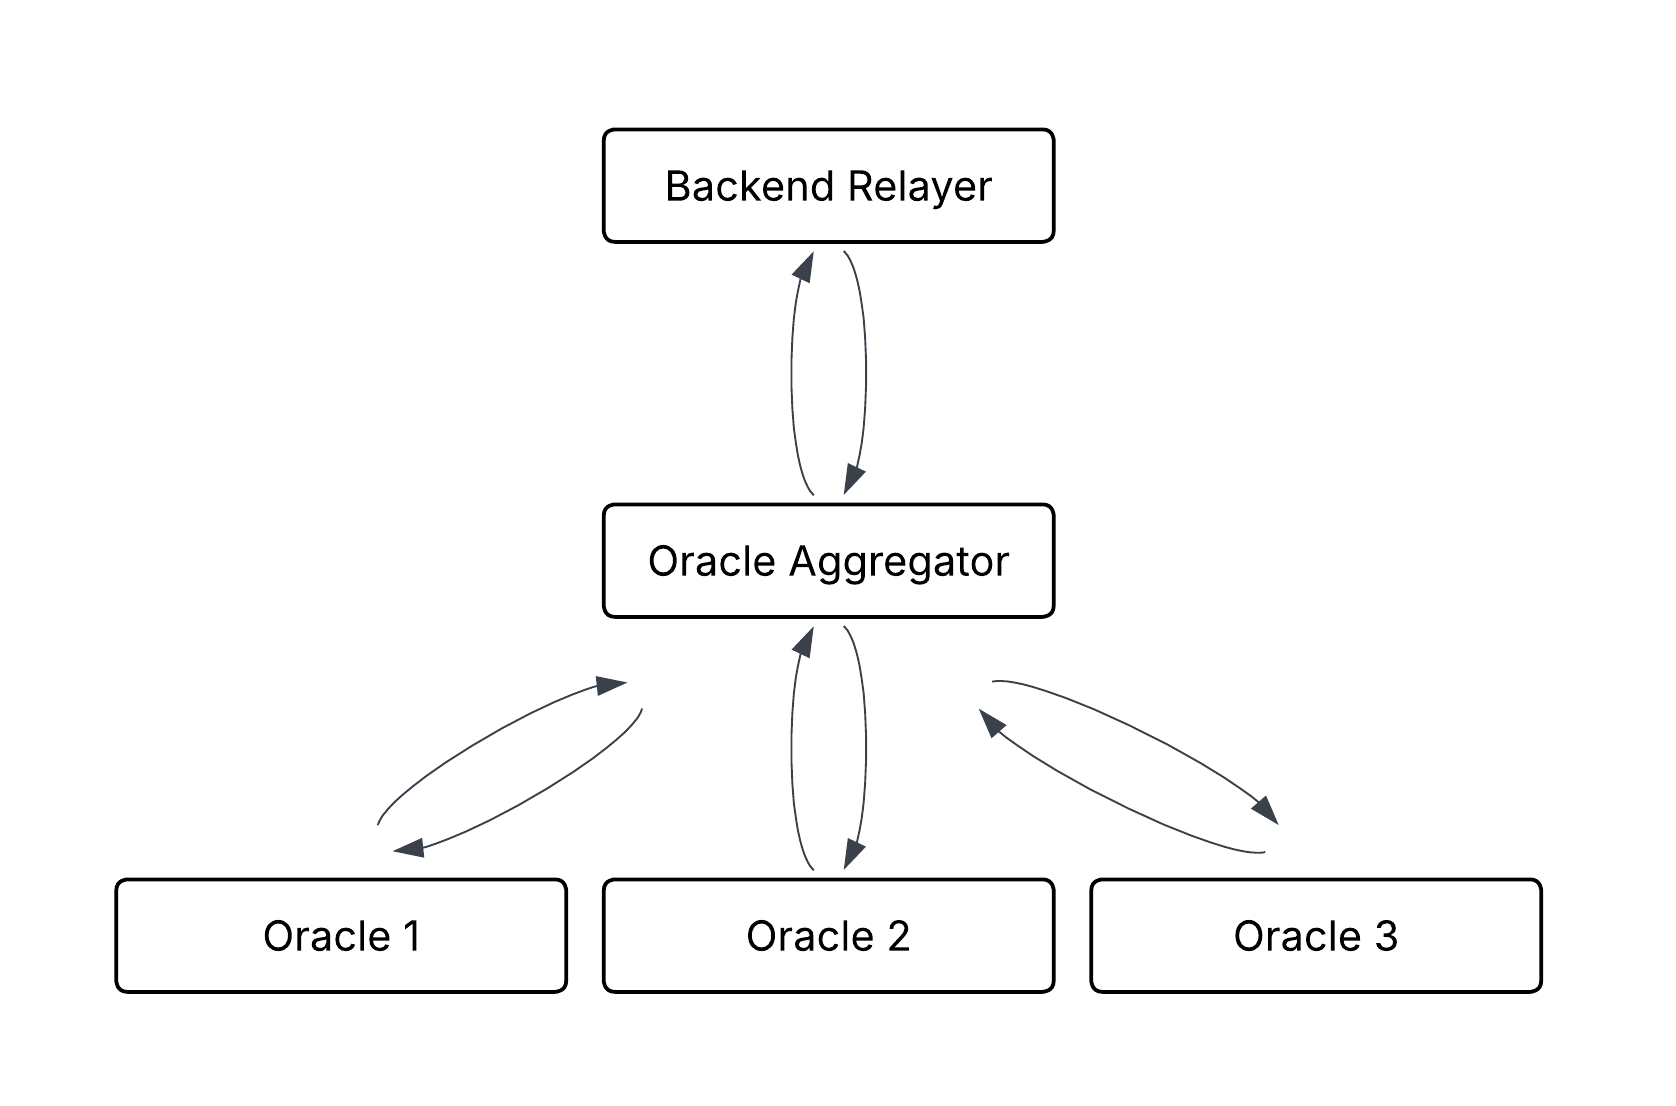
\includegraphics[width=0.95\textwidth,height=0.75\textheight,keepaspectratio]{Images/Chapter_3/oracle-architecture.png}
%     \caption{AI Content Moderation Ensemble and Oracle Aggregator Topology}
%     \label{fig:oracle-architecture}
% \end{figure}

% \subsection{Two-Tier Multi-Signature Governance \& Access Control Topology}
% \label{subsec:multisig-governance}

% In order to avoid centralised abuse of administrative powers and to ensure that the municipal authority remains accountable in a transparent way, access control is handled by means of a two-tier multi-signature governance contract, \texttt{AuthorityMultiSig.sol}, to which the ownership of \texttt{Reporting.sol} is passed when the contract is deployed. The architecture of governance divides the various stakeholders of the municipality into two separate hierarchies:

% \begin{enumerate}
%     \item \textbf{Super Admins:} A group consisting of senior municipal officials (such as the Mayor, Deputy Mayor, Chief Executive Officer, and Town Planner) who are in charge of managing the ecosystem. The Super Admins have the sole power to submit and vote on governance proposals, and the quorum is determined dynamically as a majority of the current Super Admins:
%     \begin{equation}
%         \text{Quorum} = \Big\lfloor \frac{\texttt{superAdminCount}}{2} \Big\rfloor + 1
%     \end{equation}
%     Once a proposal reaches quorum, it executes automatically.
%     \item \textbf{Authority Workers:} Municipal engineering and maintenance staff authorized to act on civic issues in \texttt{Reporting.sol} (executing \texttt{startWork}, \texttt{addAuthorityUpdate}, \texttt{markAsSolved}, and \texttt{rejectIssue}). An Authority Worker's access can be granted or revoked exclusively through Super Admin multi-sig proposals (\texttt{AddAuthority} and \texttt{RemoveAuthority}).
%     \item \textbf{On-Chain Profile Directory:} In order to ensure institutional transparency, each Super Admin and Authority Worker has an immutable on-chain identity profile (\texttt{Profile} struct) which contains their full name, official title, and the municipal department they belong to, so that citizens using the \ac{DApp} are able to check the profile of the authority assigned to deal with a civic report.
% \end{enumerate}

% When a proposal to add an authority (\texttt{AddAuthority}) or to remove an authority (\texttt{RemoveAuthority}) has achieved quorum, the contract \texttt{AuthorityMultiSig.sol} carries out a cross-contract call to the function \texttt{IReporting.setAuthority(target, authorized)}, thereby immediately updating the access registry on the main reporting contract.

% \subsection{Automated Relayer Funding \& Cron Orchestration Design}
% \label{subsec:relayer-funding-cron}

% To bridge on-chain access control with seamless off-chain operational readiness, the Backend Relayer incorporates two specialized automation services:

% \begin{enumerate}
%     \item \textbf{Authority Funding Service (\texttt{AuthorityFundingService}):}

%     Even though \texttt{AuthorityMultiSig.sol} is in charge of managing permissions, municipal staff who have been given new authority need native ETH in order to cover the cost of transaction gas on the permissioned PoA blockchain. The relayer's funding service monitors for \texttt{ProposalExecuted} events sent by \texttt{AuthorityMultiSig.sol} via WebSocket. Upon execution of an \texttt{AddAuthority} proposal, the service automatically transfers a top-up balance that can be set by the user (with a default amount of 5.0 ETH) from the pre-funded relayer treasury to the new Authority Worker's wallet. This arrangement properly separates the on-chain governance logic from the automated management of the treasury.

%     \item \textbf{Background Cron Orchestration (\texttt{CronService}):}
%     The relayer carries out two background orchestration workflows that are scheduled:
%     \begin{itemize}
%         \item \textit{Automated Balance Monitoring:} There is an automated balance monitoring system which, every day at 1 o'clock in the Colombo time zone, checks the balances of all the registered Super Admins and Authority Workers and automatically replenishes the funds of any account that falls below the minimum level required for operation (1.0 ETH).
%         \item \textit{Voting Window Batch Finalization Engine:} Even though \texttt{Reporting.sol} allows for lazy evaluation in the case of a user submitting a vote after the phase deadline, reports that have no further voting activity could stay indefinitely in a pending state. In order to avoid workflow stagnation, a daily cron job that runs at midnight checks the blockchain for reports which are in voting phases ($S_0 = \texttt{PendingValidation}$, $S_4 = \texttt{PendingRejectionReview}$, or $S_5 = \texttt{PendingVerification}$) where $\text{block.timestamp} > \texttt{phaseDeadline}$ and for which block.timestamp is greater than the phaseDeadline. The cron service then carries out a batch transaction by calling \texttt{batchFinalizeVotingWindows} for all reports that have expired, thereby forcing deterministic state transitions throughout the platform.
%     \end{itemize}
% \end{enumerate}

% \subsection{Private Permissioned Validator Network Topology}
% \label{subsec:validator-topology}

% The basic ledger functions as a private, permissioned network that is compatible with Ethereum and uses the Clique \ac{PoA} consensus protocol. In order to achieve distributed governance without having to incur the energy use and latency associated with Proof-of-Work (\ac{PoW}), authority for sealing blocks is limited to a group of institutional validator nodes which have been previously approved. This group consists of three main validator nodes:


% \begin{itemize}
%     \item \textbf{Municipal Authority Validator Node:} Hosted by local government administrative departments responsible for infrastructure maintenance.
%     \item \textbf{Regional Oversight Validator Node:} Managed by regional or provincial supervisory bodies to ensure inter-agency auditing.
%     \item \textbf{Independent Civic NGO Validator Node:} Operated by recognized civil society organizations to maintain democratic equilibrium and prevent unilateral censorship by government nodes.
% \end{itemize}

% Figure~\ref{fig:validator-nodes} illustrates the 3-validator network topology, depicting inter-node peer connections, RPC endpoint access, and block propagation paths.

% \begin{figure}[!htbp]
%     \centering
%     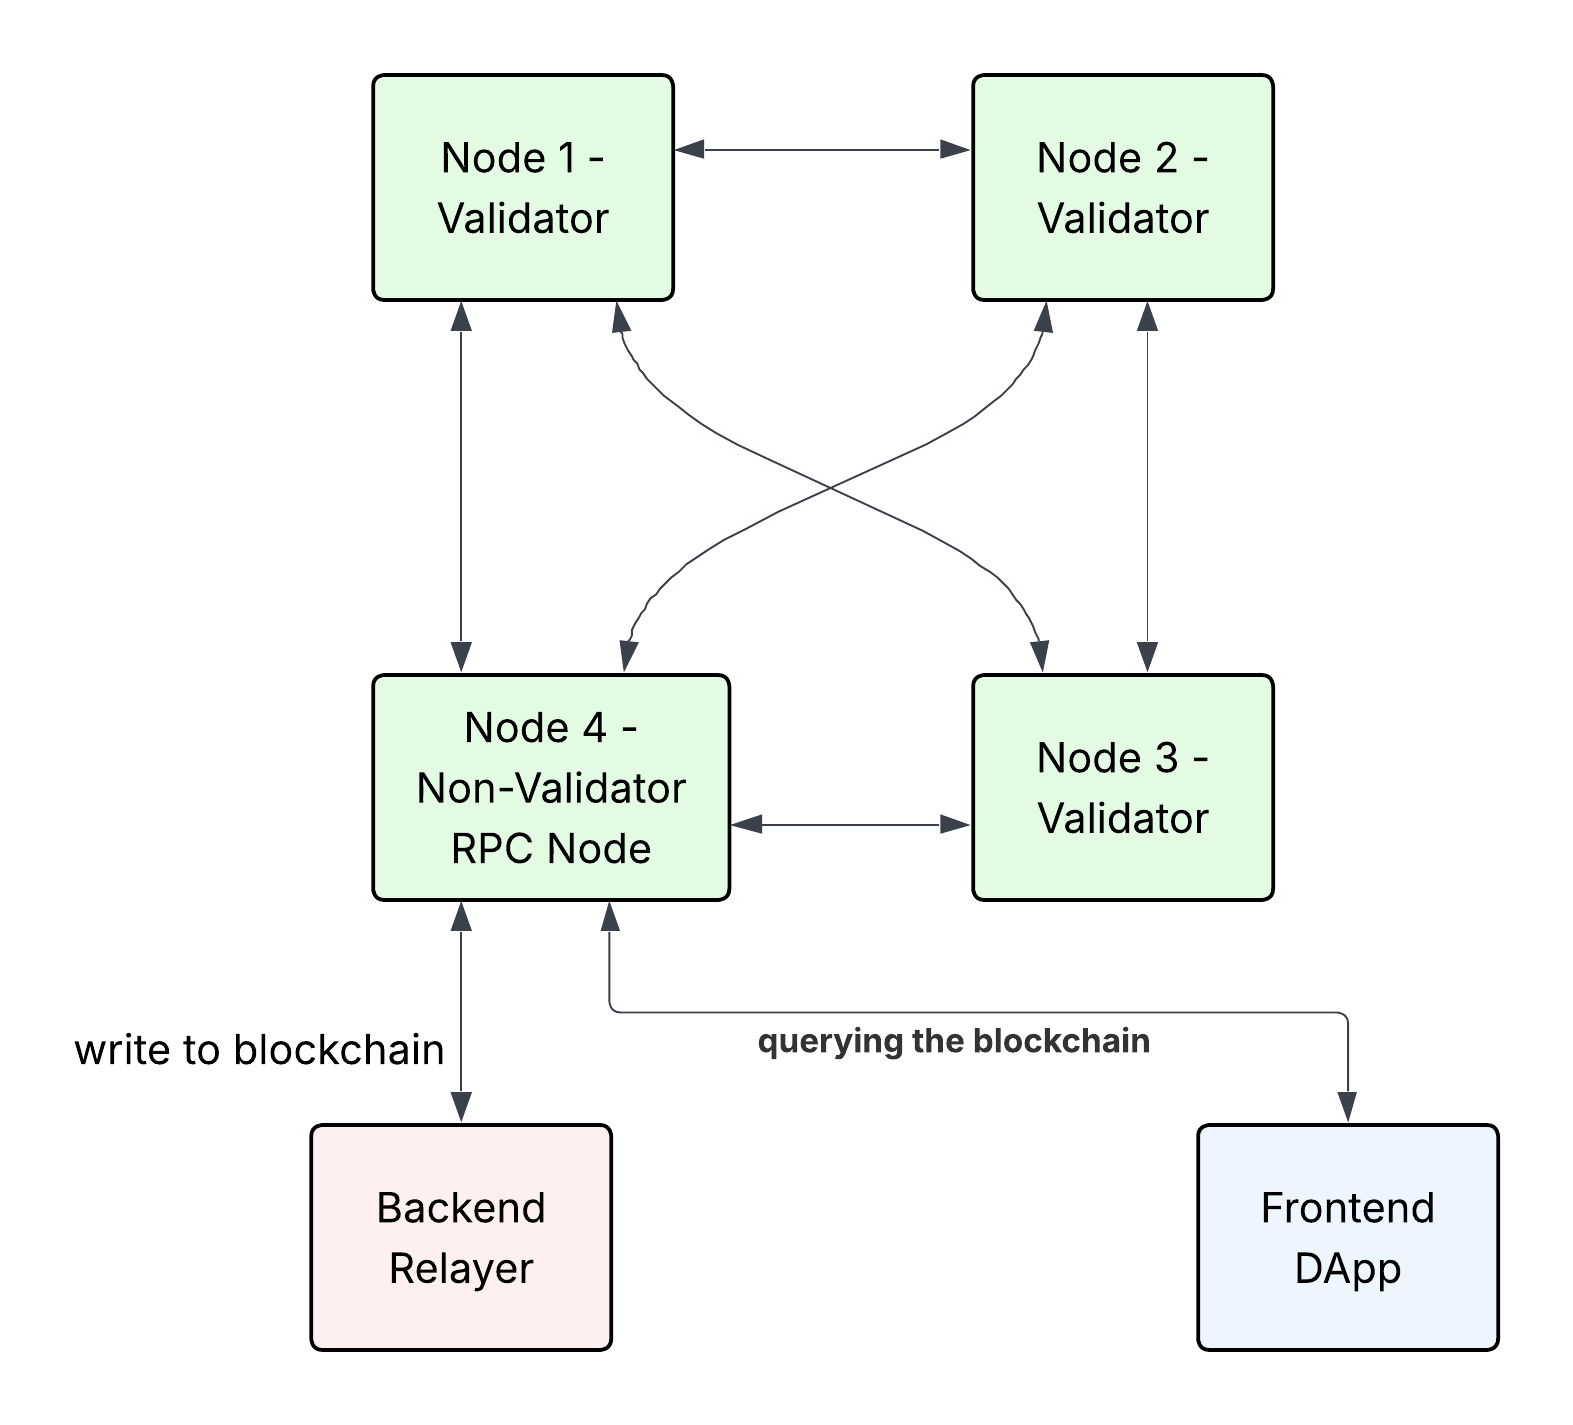
\includegraphics[width=0.95\textwidth,height=0.75\textheight,keepaspectratio]{Images/Chapter 3/validator_nodes.png}
%     \caption{Private Permissioned Proof-of-Authority (PoA) Validator Network Topology}
%     \label{fig:validator-nodes}
% \end{figure}

% \section{Detailed Workflow \& Finite State Machine (FSM) Design}
% \label{sec:detailed-workflow-fsm}

% The operational principles at the heart of the platform are expressed in the form of a mathematical Finite State Machine (\ac{FSM}) and are implemented in the \texttt{Reporting.sol} smart contract. The following section describes the state transitions, the cryptographic nullifier safeguards, and the deterministic procedures that oversee a civic report from the moment it is submitted until its verification after resolution.

% \subsection{Finite State Machine (FSM) Overview}
% \label{subsec:fsm-overview}

% A civic issue report is modeled as an eight-state deterministic \ac{FSM}. Let $\mathcal{S}$ define the discrete set of legal report states:
% \begin{equation}
%     \mathcal{S} = \big\{ S_0, S_1, S_2, S_3, S_4, S_5, S_6, S_7 \big\}
% \end{equation}
% where:
% \begin{itemize}
%     \item $S_0 = \texttt{PendingValidation}$: The initial state upon on-chain submission; the report is accessible on the community feed for peer validation voting within a 6-hour window.
%     \item $S_1 = \texttt{CommunityRejected}$: A terminal state reached if community downvotes exceed upvotes during the validation phase.
%     \item $S_2 = \texttt{Open}$: An active state entered when a report achieves community consensus; the issue becomes actionable for municipal authorities.
%     \item $S_3 = \texttt{InProgress}$: An active state entered when an assigned authority claims the report and begins physical infrastructure repairs.
%     \item $S_4 = \texttt{PendingRejectionReview}$: A review state entered if an authority rejects an issue as invalid; the community is granted a 6-hour window to uphold or appeal the rejection.
%     \item $S_5 = \texttt{PendingVerification}$: A verification state entered after an authority marks an issue as solved; citizens physically inspect the repair and cast accept/reject votes within a 6-hour window.
%     \item $S_6 = \texttt{Closed}$: A terminal state indicating that an issue has been successfully resolved and community-verified, or that an authority rejection was upheld.
%     \item $S_7 = \texttt{Reopened}$: An active state triggered if the community rejects a claimed repair during verification or successfully appeals an authority rejection.
% \end{itemize}

% State transitions are protected by role-based access control (\ac{RBAC}), by constraints relating to the temporal window ($\Delta t_{\text{window}} = 6\text{ hours}$), and by cryptographic nullifier tracking. In order to prevent Sybil attacks and double voting, the smart contract keeps record of the hashes of the tickets in permanent mappings (\texttt{usedSubmissionNullifiers}, \texttt{usedValidationVoteNullifiers}, \texttt{usedVerificationVoteNullifiers}, and \texttt{usedRejectionReviewVoteNullifiers}), thereby adhering to the Checks-Effects-Interactions (CEI) design pattern.

% Figure~\ref{fig:state-transition-diagram} presents the formal state transition diagram of the reporting \ac{FSM}, while Figure~\ref{fig:overall-workflow} illustrates the end-to-end lifecycle workflow of a civic issue across all system components.

% \begin{figure}[!htbp]
%     \centering
%     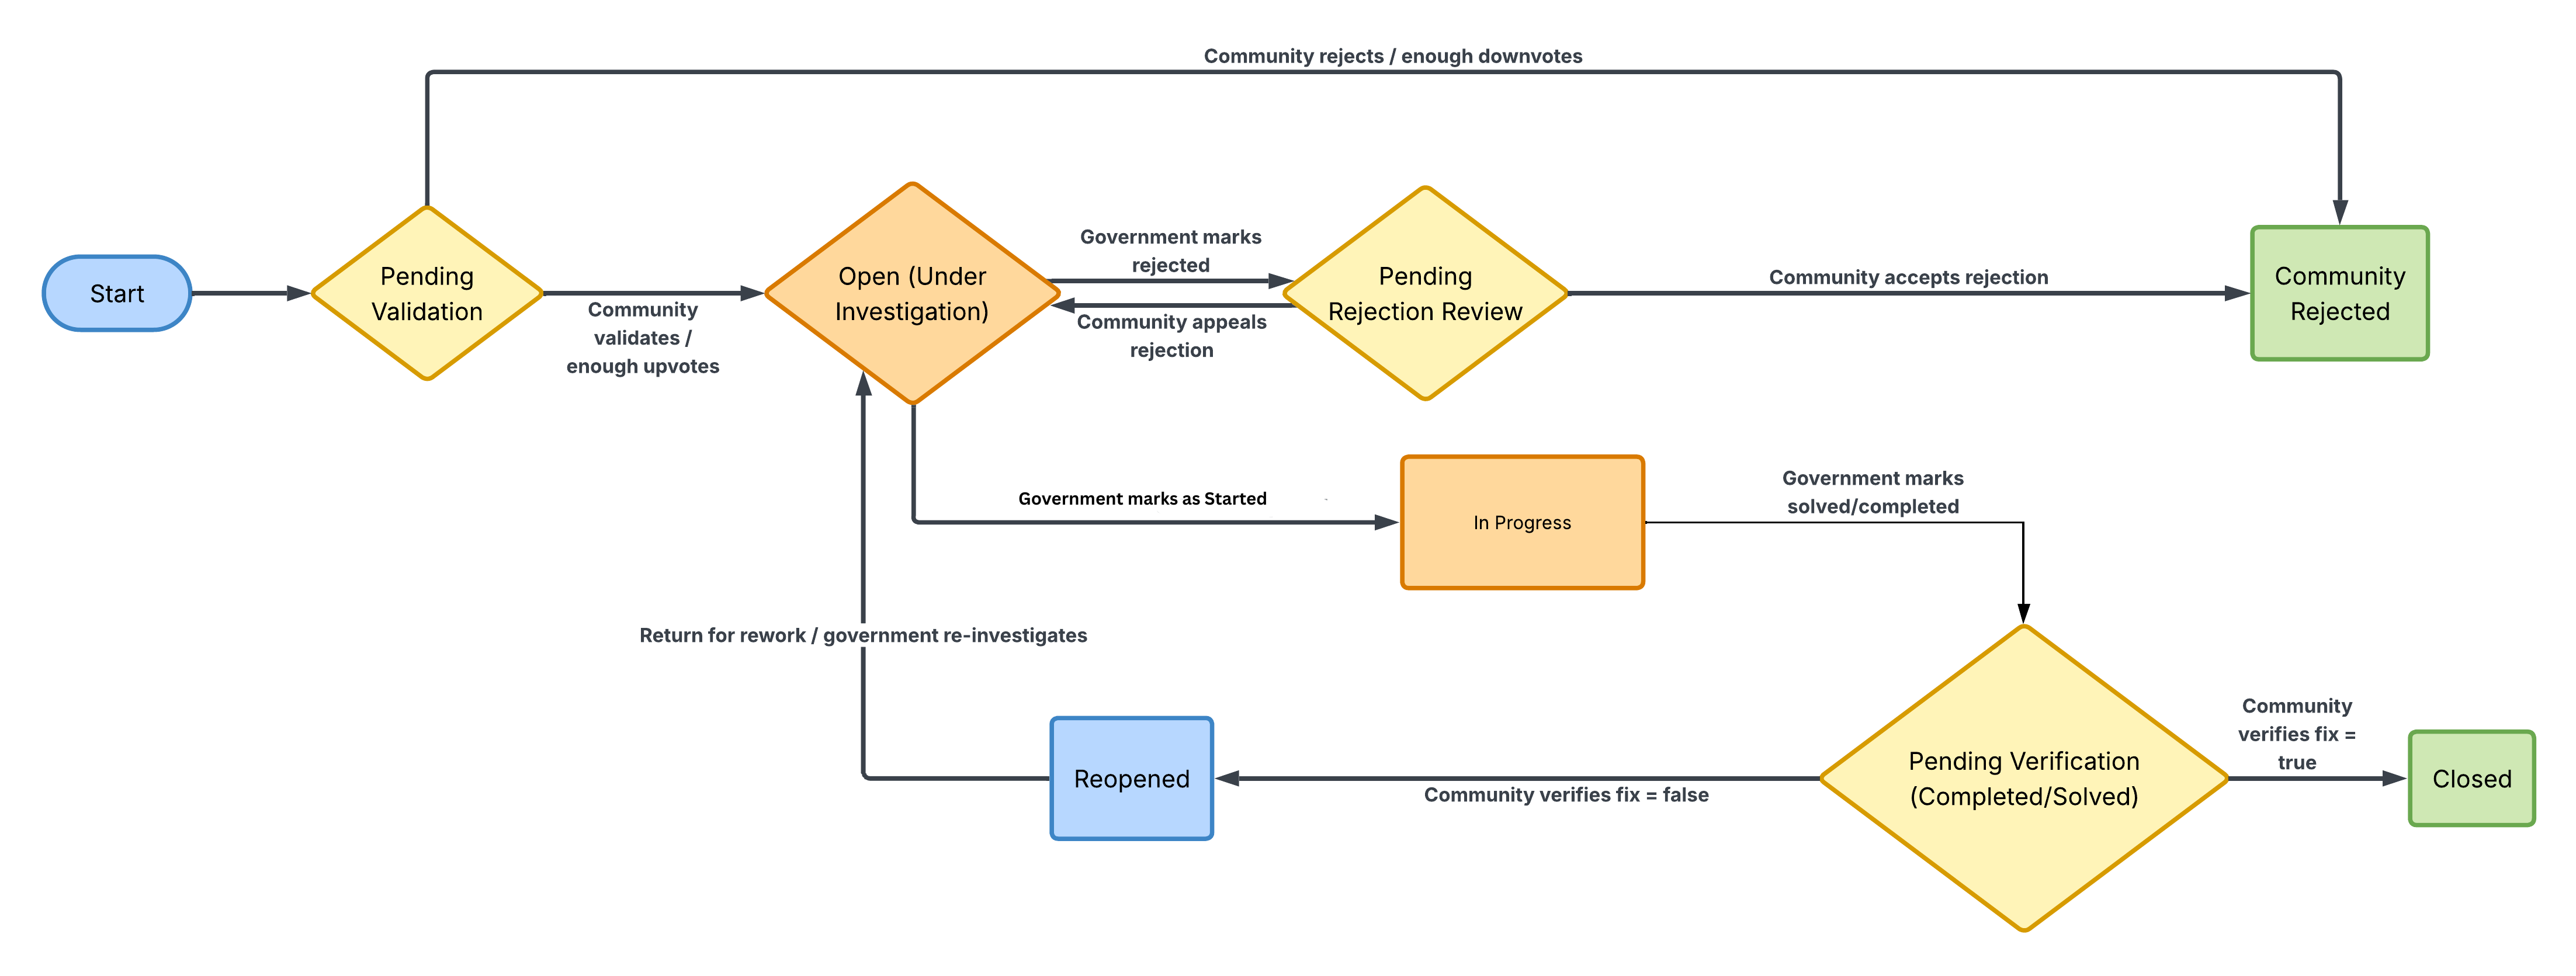
\includegraphics[width=0.95\textwidth,height=0.75\textheight,keepaspectratio]{Images/Chapter 3/state-transition-diagram-3.png}
%     \caption{Finite State Machine (FSM) State Transition Diagram for Civic Reports}
%     \label{fig:state-transition-diagram}
% \end{figure}

% \begin{figure}[!htbp]
%     \centering
%     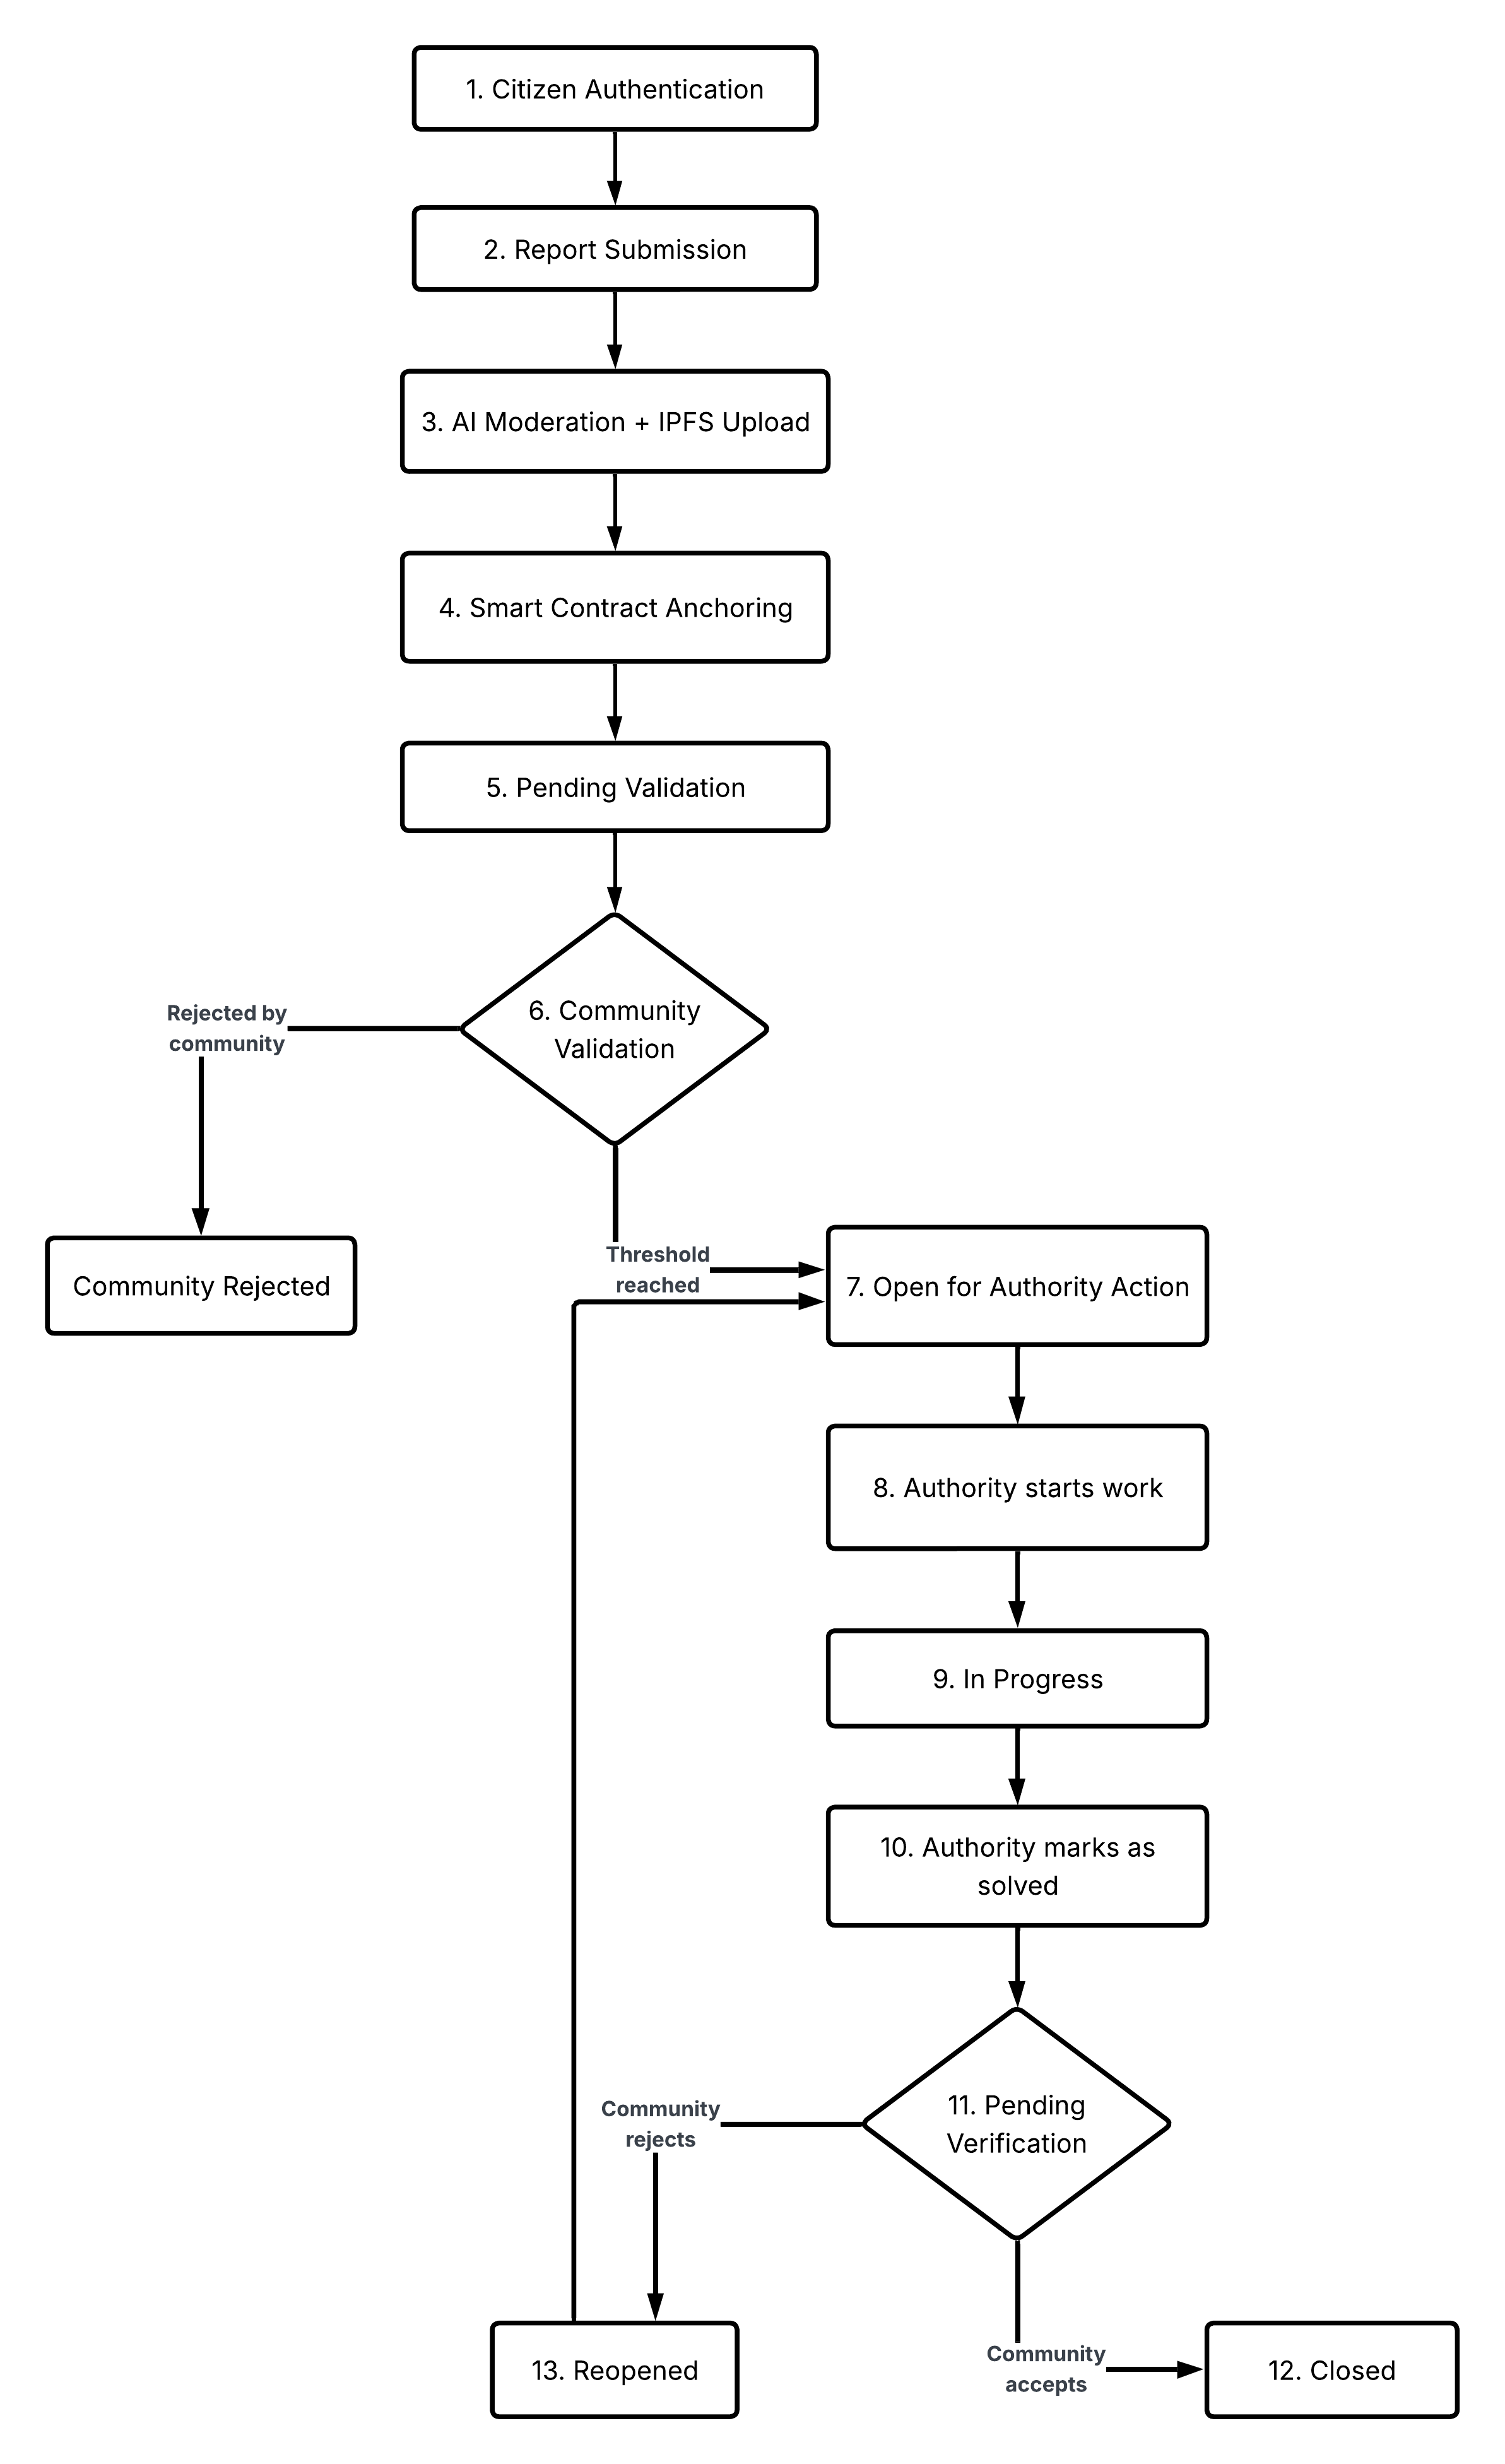
\includegraphics[width=0.95\textwidth,height=0.75\textheight,keepaspectratio]{Images/Chapter 3/overall_reporting_workflow.png}
%     \caption{Overall Lifecycle Workflow of a Civic Issue Within the Decentralized Ecosystem}
%     \label{fig:overall-workflow}
% \end{figure}

% \subsection{Citizen Authentication \& Identity Decoupling Workflow}
% \label{subsec:auth-workflow}

% The authentication workflow separates a citizen's real-world civic identity from their actions on the chain, thus avoiding the linking of transactions while at the same time making sure that only eligible citizens can take part. Figure~\ref{fig:authentication-workflow} shows the sequential steps in the authentication and credential issuance process. The authentication workflow involves five definite steps:

% \begin{figure}[!htbp]
%     \centering
%     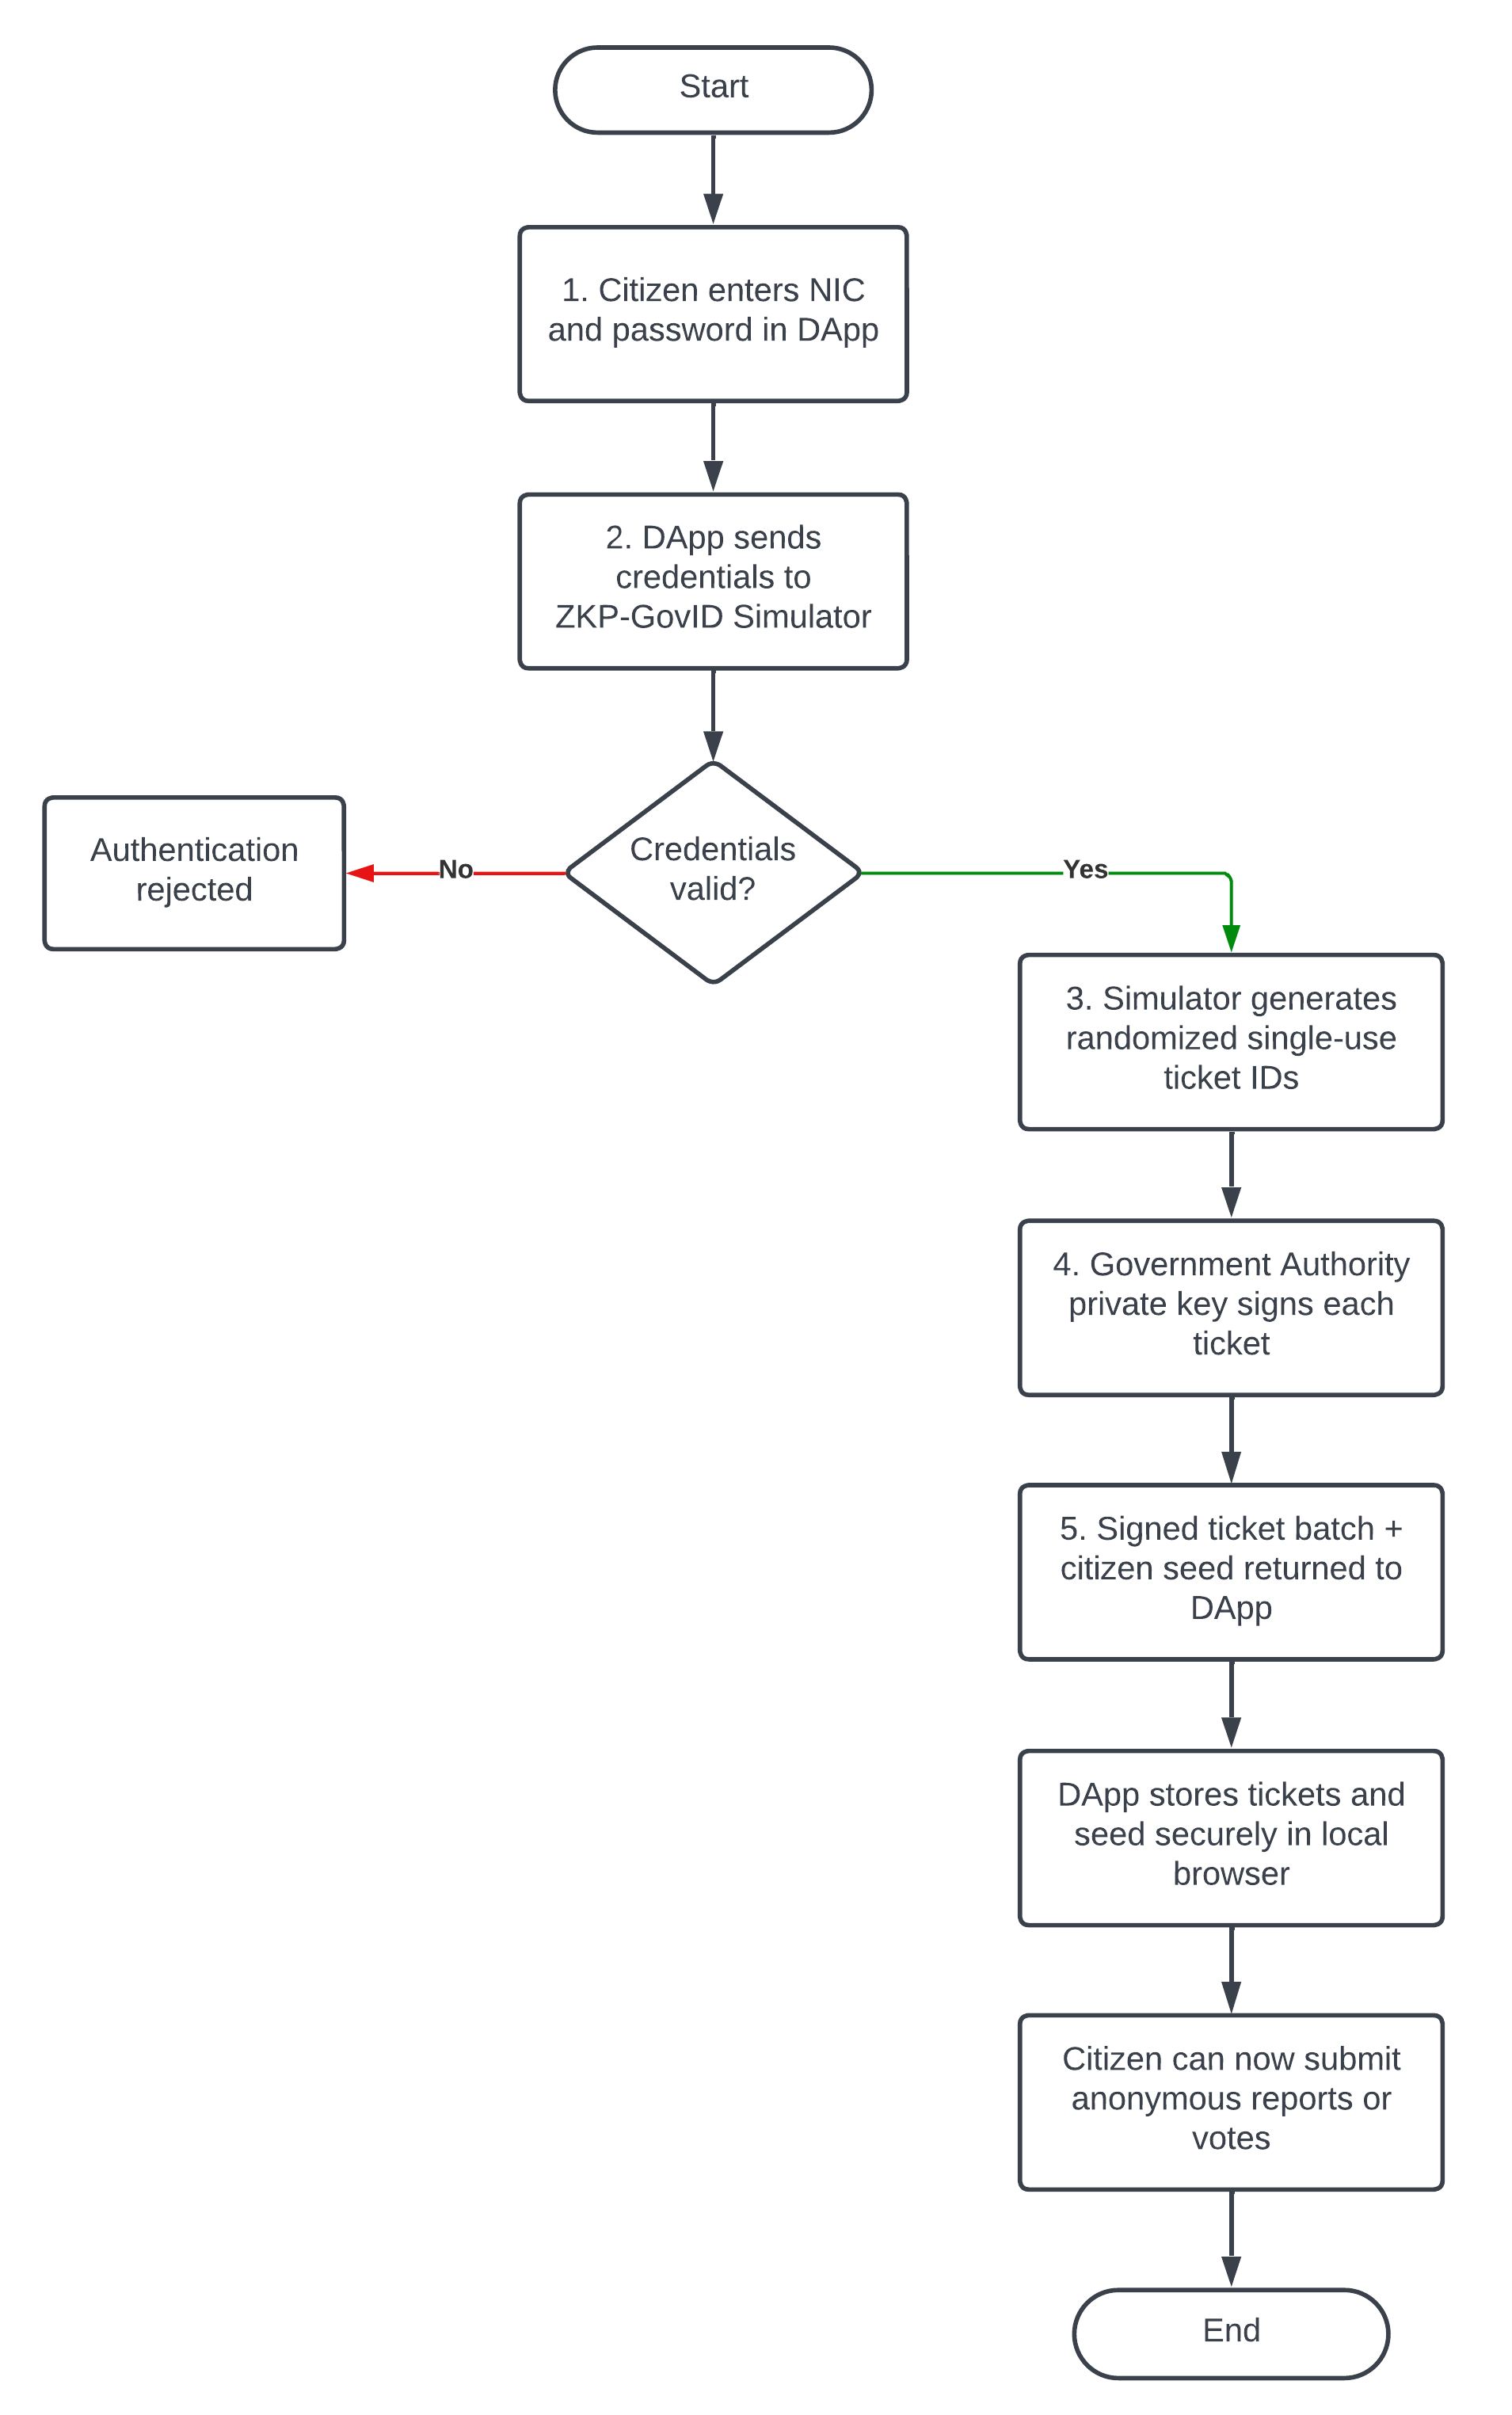
\includegraphics[width=0.95\textwidth,height=0.75\textheight,keepaspectratio]{Images/Chapter 3/authentication_workflow.png}
%     \caption{Citizen Authentication and Identity Decoupling Workflow}
%     \label{fig:authentication-workflow}
% \end{figure}

% The authentication workflow proceeds through five deterministic steps:
% \begin{enumerate}
%     \item \textbf{Submission of credentials:} the citizen enters their official National Identity Number (NID) and password into the \ac{DApp} login interface.
%     \item \textbf{For zero-knowledge verification,} the \ac{DApp} sends an authentication request to the ZKP GovID Simulator, which checks the credentials against the fake government database without either revealing or keeping any sensitive identification attributes.
%     \item \textbf{Ticket Batch Generation:} After the verification has been successfully carried out, the simulator produces a batch consisting of ten randomly generated, single-use ticket identifiers ($\texttt{zkpTicketId}_1, \dots, \texttt{zkpTicketId}_{10}$) together with a unique citizen seed.
%     \item \textbf{Cryptographic signing:} Each ticket identifier is cryptographically signed by the simulator using the private key of the government authority, thus providing proof of validity.
%     \item \textbf{Local Browser Storage:} The signed ticket batch and the citizen seed are sent back to the client and stored securely in the browser's local storage. In order to enable on-chain tracking of individual submissions, the client generates a deterministic citizen pseudonym that is unlinkable:
%     \begin{equation}
%         \text{Pseudonym} = \text{keccak256}\Big(\text{citizenPubKey} \parallel \text{DOMAIN\_SALT}\Big)
%     \end{equation}
% \end{enumerate}

% \subsection{Report Submission \& Moderation Pipeline}
% \label{subsec:submission-pipeline}

% The workflow for submitting reports involves carrying out cryptographic signing on the client side, having the relayer verify it, subjecting the content to AI moderation, storing it off-chain using \ac{IPFS}, and then anchoring the transaction on the chain. Figure~\ref{fig:report-submission-workflow} shows the entire report submission and moderation pipeline.

% \begin{figure}[!htbp]
%     \centering
%     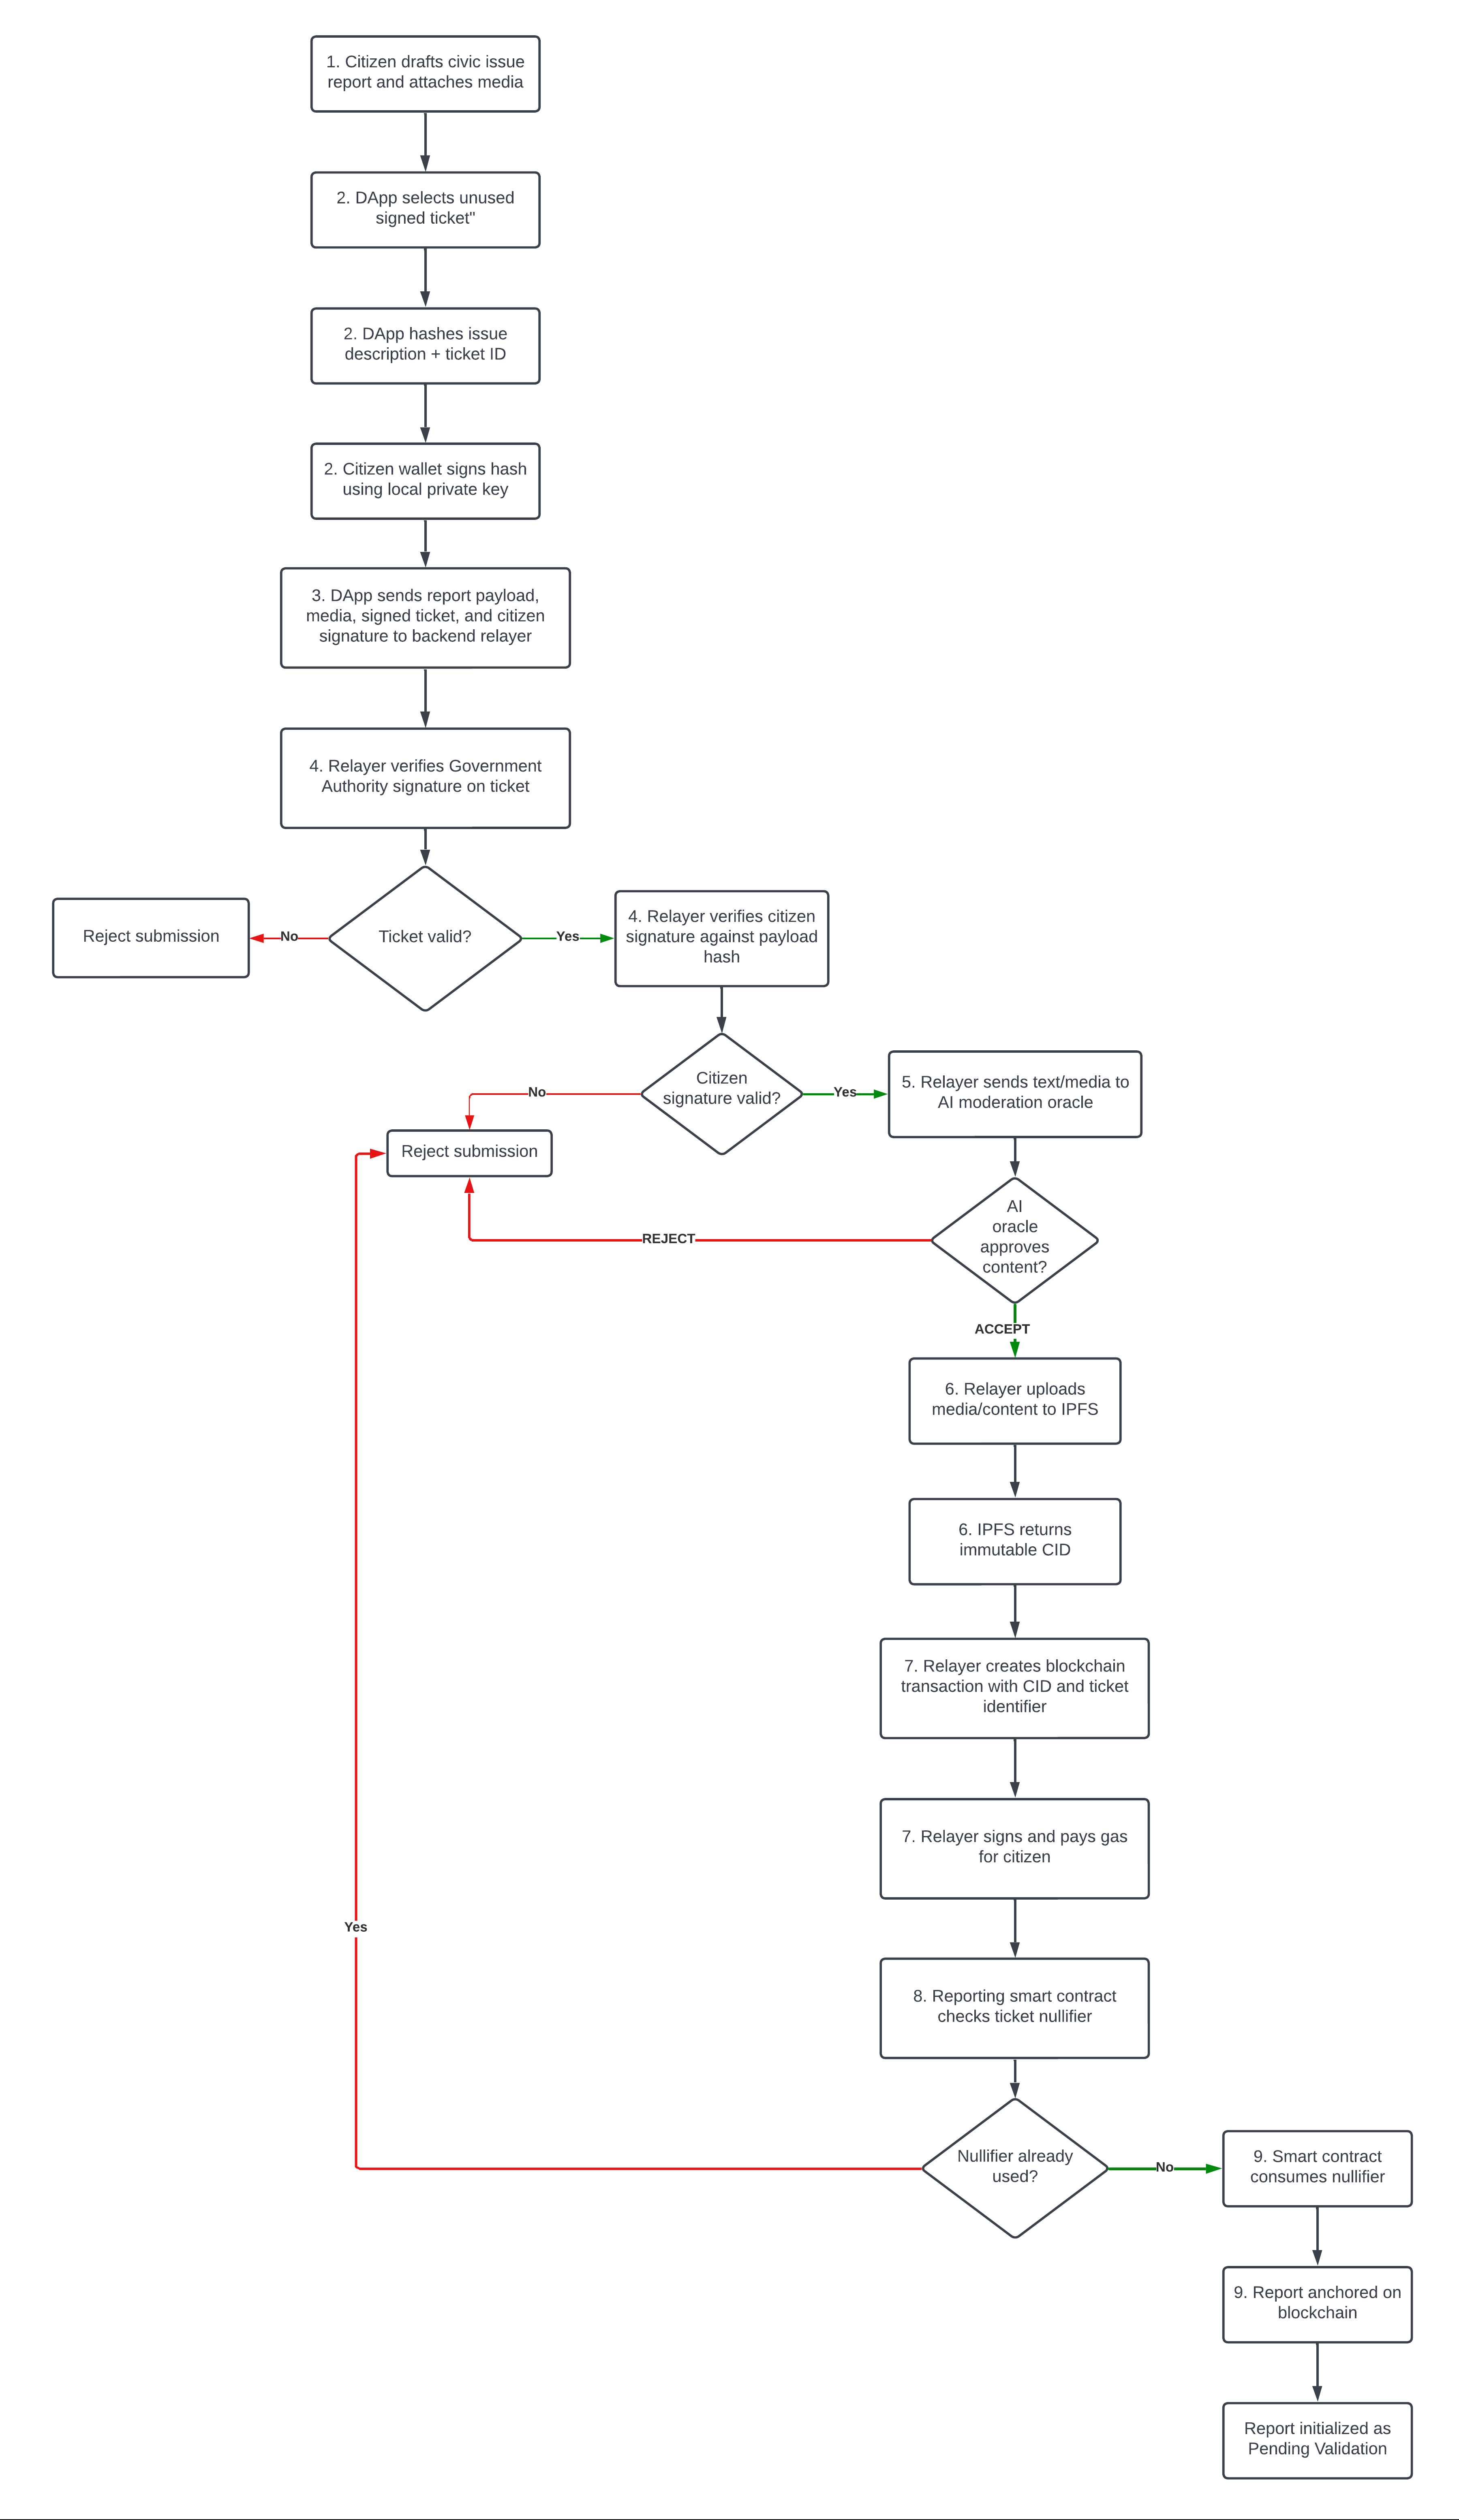
\includegraphics[width=0.95\textwidth,height=0.75\textheight,keepaspectratio]{Images/Chapter 3/report_submission_workflow.png}
%     \caption{Report Submission, AI Moderation, and Blockchain Anchoring Pipeline}
%     \label{fig:report-submission-workflow}
% \end{figure}

% The submission pipeline executes as follows:
% \begin{enumerate}
%     \item \textbf{Payload Structuring and Signing:} When structuring and signing the payload, the citizen chooses an issue category, types in a textual description, and attaches any optional media evidence. The \ac{DApp} then calculates the composite report hash ($\mathcal{H}_{\text{report}}$), signs it with the citizen's ephemeral private key, and picks an unused signed ticket from local storage.
%     \item \textbf{Relayer Transmission:} The \ac{DApp} sends to the Backend Relayer via an HTTPS POST the entire payload, which includes the raw text, the media files, the government-signed ticket, and the citizen's signature.
%     \item \textbf{Cryptographic Payload Verification:} The relayer checks that the ticket signature is associated with the government authority and that the citizen's signature corresponds to the report hash. The request is then rejected right away if this verification fails.
%     \item \textbf{AI Content Moderation:} The relayer sends the text and media on to the AI Moderation Ensemble, which then assesses the submission using the toxicity, spam, and civic relevance classifiers. The Oracle Aggregator acts on the evaluation and, if the ensemble decides to reject the submission, the relayer aborts it and sends back a descriptive error to the \ac{DApp}.
%     \item \textbf{IPFS Content Anchoring:} Upon receiving an \texttt{ACCEPT} verdict, the relayer uploads the report text and media files to \ac{IPFS}, obtaining the immutable Content Identifier (\texttt{ipfsCid}).
%     \item \textbf{On-Chain Transaction Submission:} When submitting the on-chain transaction, the relayer creates a transaction which calls the \texttt{submitReport} function on \texttt{Reporting.sol} and includes the \texttt{ipfsCid}, $\mathcal{H}_{\text{report}}$, the hash of the single-use ticket as the \texttt{submissionNullifier}, and the citizen's derived pseudonym. The relayer then signs this transaction using its own wallet and pays the associated gas costs.
%     \item \textbf{Smart Contract Nullifier Enforcement:} The smart contract looks at the value of \texttt{usedSubmissionNullifiers[submissionNullifier]}. If that nullifier has already been used, the transaction is reverted; otherwise, the contract records the nullifier as having been used, places the report into state $S_0 (\texttt{PendingValidation})$, sets the phase deadline to $\text{block.timestamp} + 6\text{ hours}$, and sends out the \texttt{ReportSubmitted} event.
% \end{enumerate}

% \subsection{Community Consensus \& Validation Workflow}
% \label{subsec:validation-workflow}

% In order to filter out spam and make sure that only real civic concerns are passed on to the municipal authorities, reports that have just been submitted go through a process of community validation. Figure~\ref{fig:community-validation-workflow} shows the workflow for reaching a community consensus and for peer validation.

% \begin{figure}[!htbp]
%     \centering
%     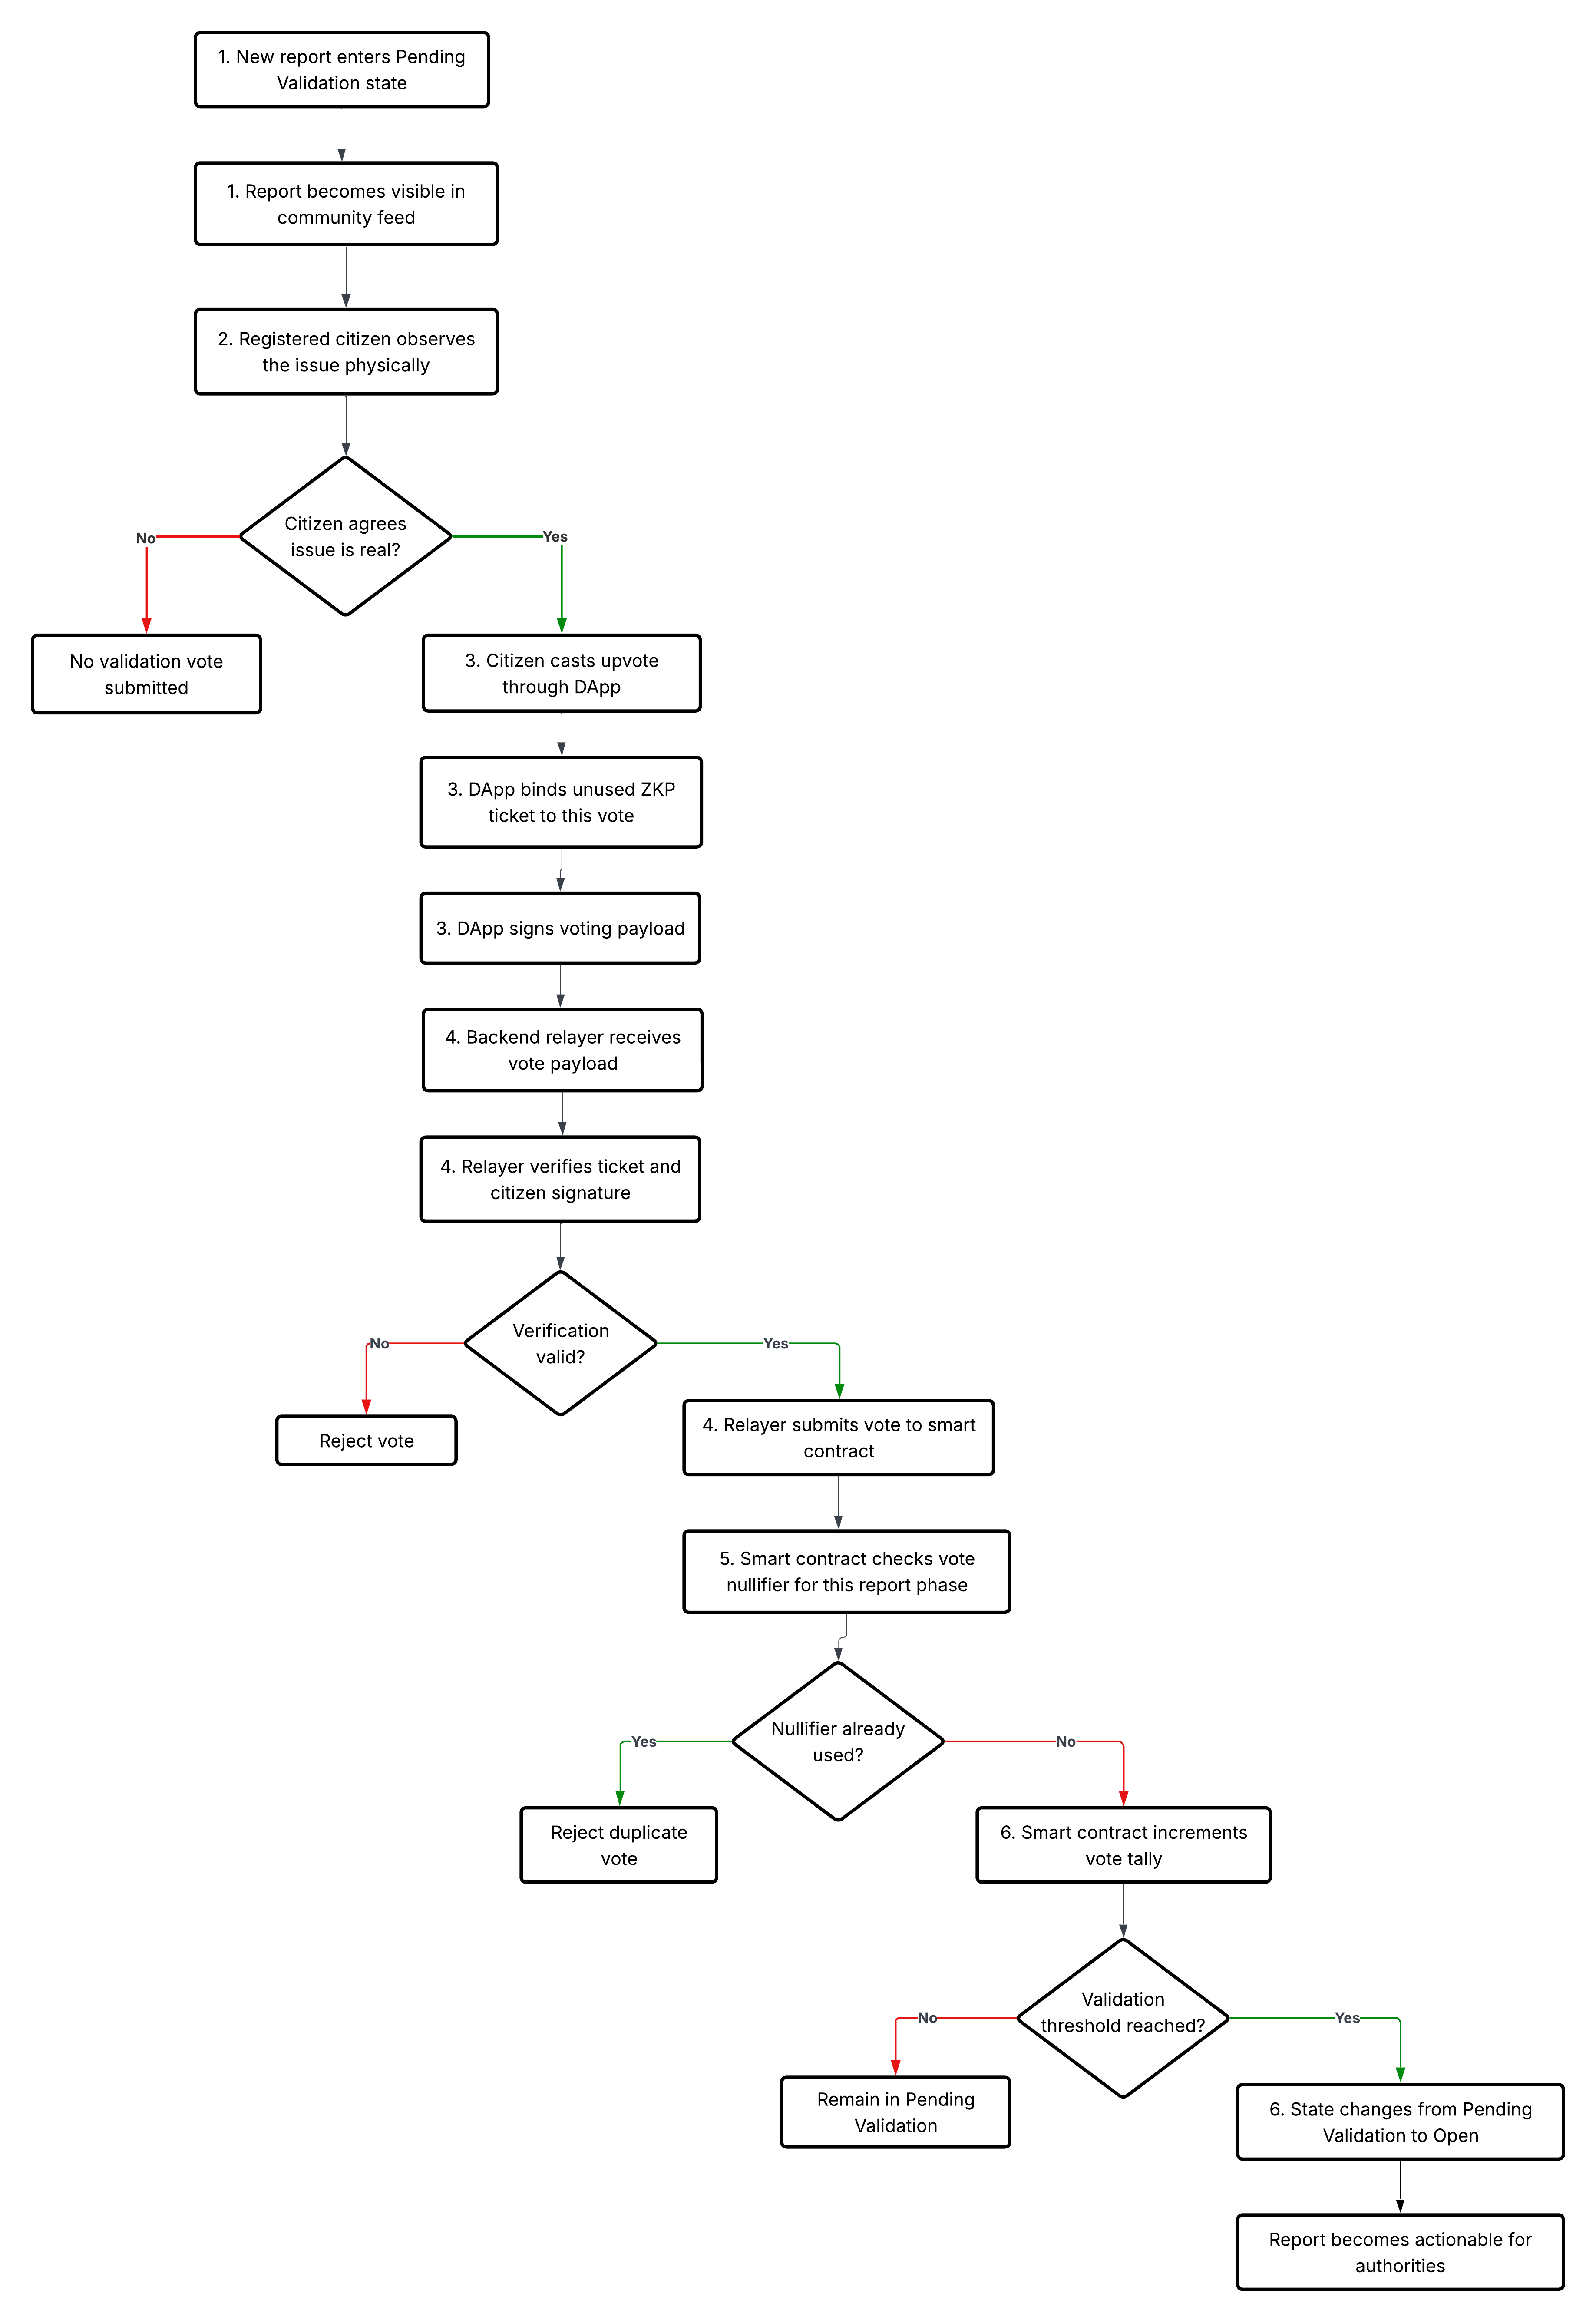
\includegraphics[width=0.95\textwidth,height=0.75\textheight,keepaspectratio]{Images/Chapter 3/community_validation_workflow.png}
%     \caption{Community Consensus and Peer-Validation Workflow}
%     \label{fig:community-validation-workflow}
% \end{figure}

% The validation workflow proceeds as follows:
% \begin{enumerate}
%     \item \textbf{Community Feed Visualization:} The public \ac{DApp} feed shows reports that are in state $S_0 (\texttt{PendingValidation})$ together with an active countdown timer indicating the 6-hour voting period.
%     \item \textbf{Sybil-Resistant Vote Casting:} To ensure sybil resistance, citizens look at the report and carry out an upvote ($\texttt{support} = \text{true}$) or a downvote ($\texttt{support} = \text{false}$) by using a nullifier of an unused ticket.
%     \item \textbf{Relayer Signature and Ticket Validation:} The relayer verifies the citizen's vote payload and forwards the transaction to \texttt{castValidationVote} on \texttt{Reporting.sol}.
%     \item \textbf{On-Chain Vote Tallying:} When tallying the on-chain votes, the smart contract checks that \texttt{usedValidationVoteNullifiers[reportId][voteNullifier]} is false, uses the nullifier, and then increases the appropriate count, either \texttt{validationUpvotes} or \texttt{validationDownvotes}.
%     \item \textbf{State Finalization Engine:} State finalization occurs through two complementary mechanisms:
%     \begin{itemize}
%         \item \textit{Lazy Evaluation:} If any user submits a vote after the deadline ($\text{block.timestamp} > \texttt{phaseDeadline}$), the contract will automatically call \texttt{\_finalizeSingleReport}.
%         \item \textit{Automated Cron Finalization:} If no user action occurs, the relayer's background \texttt{CronService} invokes \texttt{batchFinalizeVotingWindows} daily at midnight, ensuring timely transitions.
%     \end{itemize}
%     If $\texttt{upvotes} > \texttt{downvotes}$, the report moves into state $S_2 (\texttt{Open})$; otherwise, it moves into state $S_1 (\texttt{CommunityRejected})$.
% \end{enumerate}

% \subsection{Authority Resolution \& Action Workflow}
% \label{subsec:authority-workflow}

% Reports which reach a consensus within the community ($S_2 = \texttt{Open}$) become actionable for municipal authorities. Figure~\ref{fig:authority-action-workflow} sets out the procedure for authority resolution, work tracking, and status updates.

% \begin{figure}[!htbp]
%     \centering
%     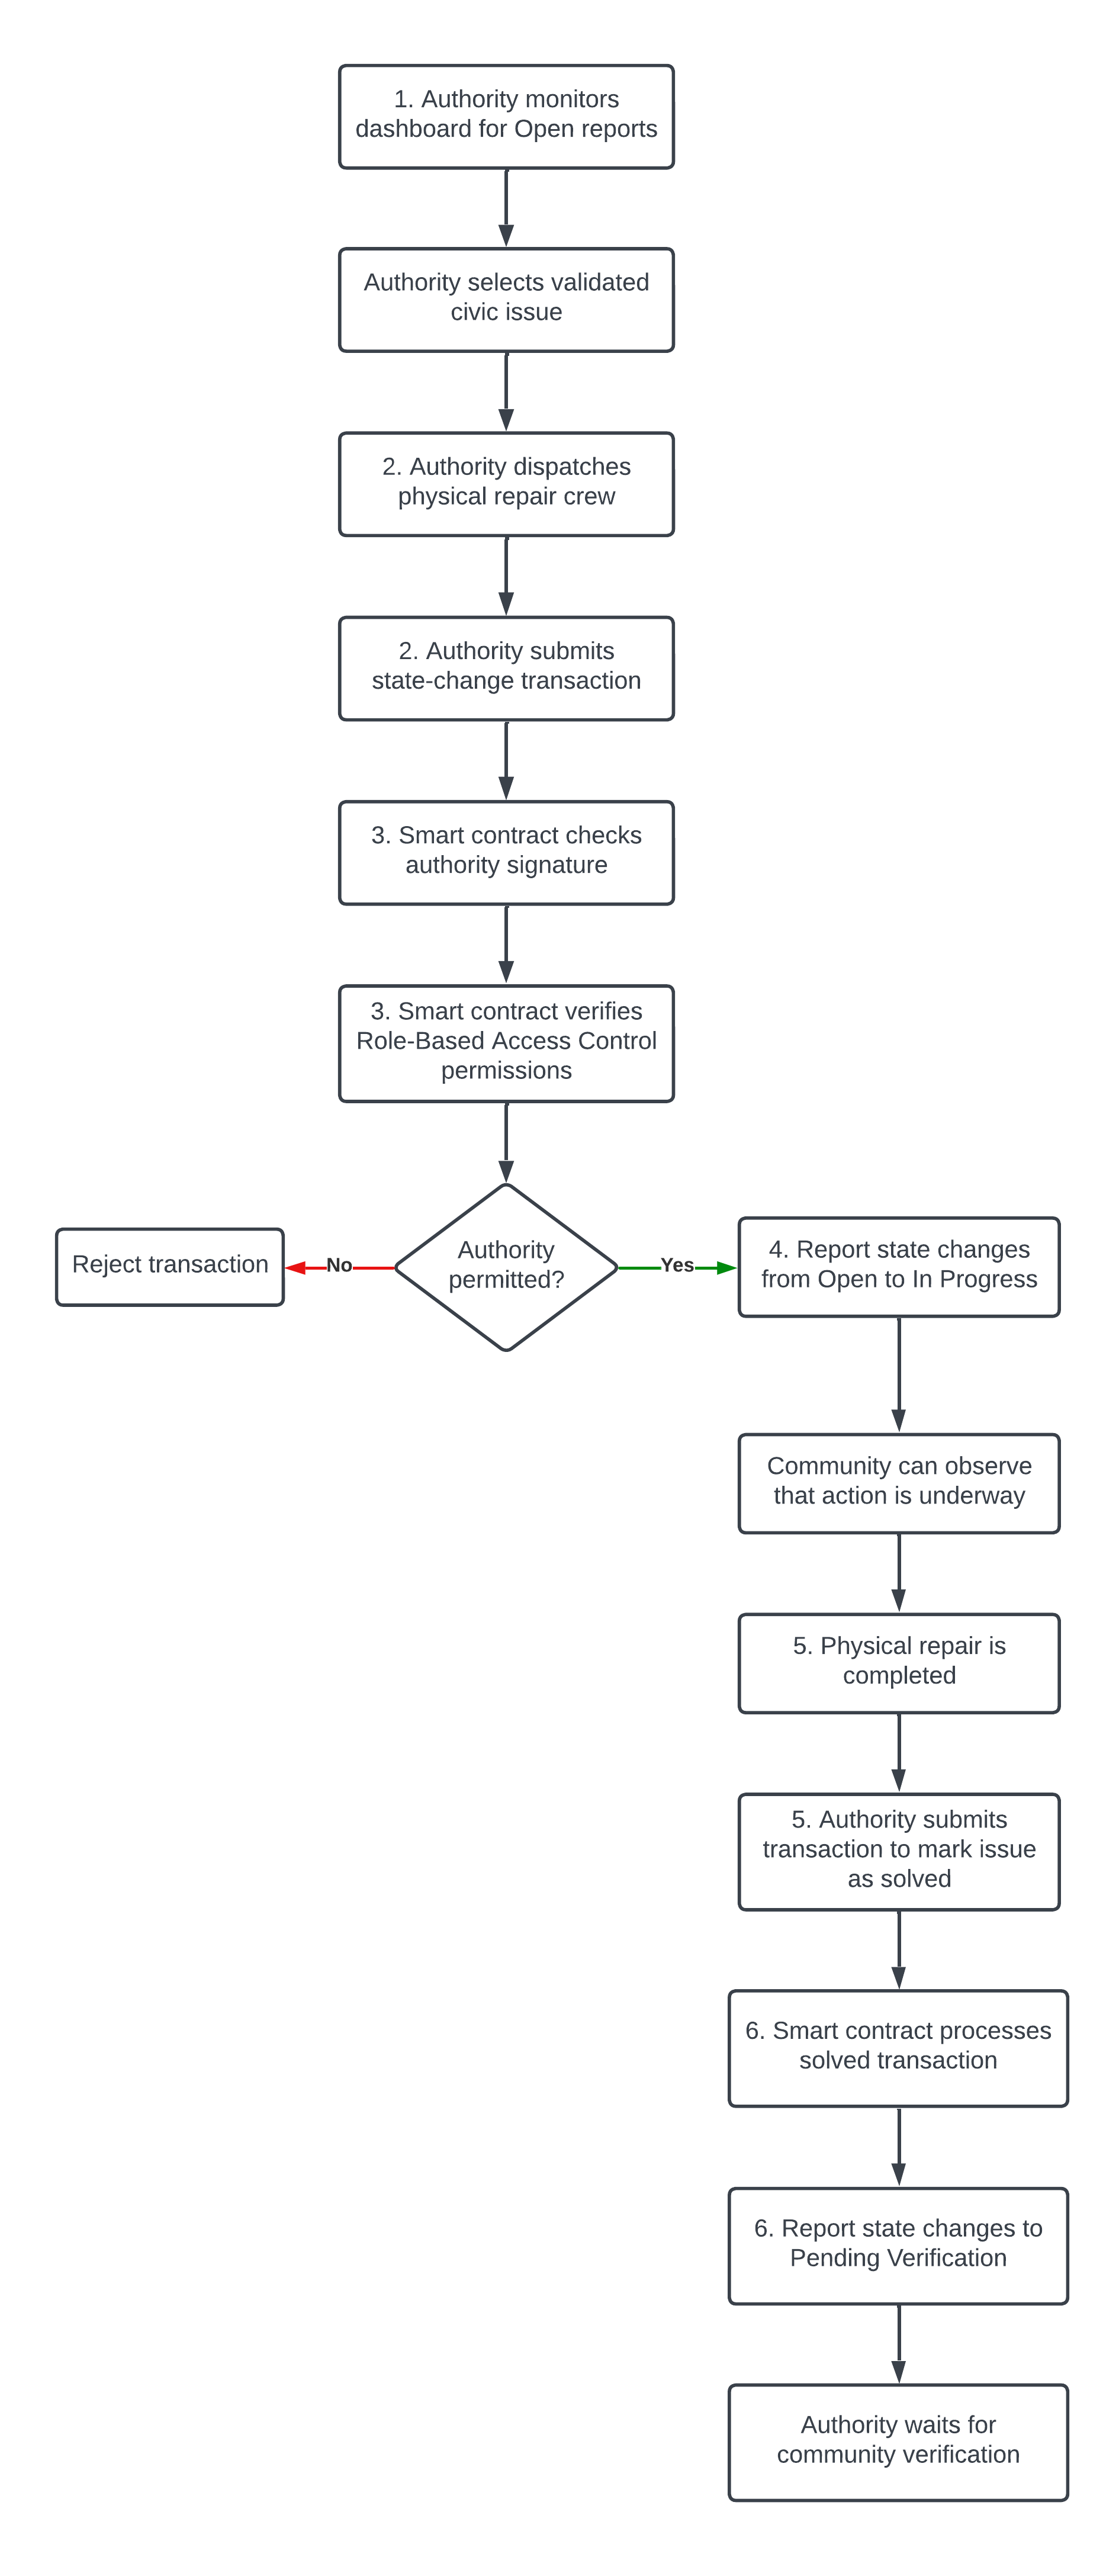
\includegraphics[width=0.95\textwidth,height=0.75\textheight,keepaspectratio]{Images/Chapter 3/authority_action_workflow.png}
%     \caption{Authority Resolution and Infrastructure Repair Workflow}
%     \label{fig:authority-action-workflow}
% \end{figure}

% The authority workflow executes through the following operations:
% \begin{enumerate}
%     \item \textbf{Dashboard monitoring and profile verification:} Authorized municipal officials can monitor validated reports through the authenticated Authority Dashboard within the \ac{DApp}, and when an authority carries out an interaction with a report, their on-chain identity profile (including \texttt{name}, \texttt{position} and \texttt{department}) which is managed by \texttt{AuthorityMultiSig.sol} is shown to the community.
%     \item \textbf{Work Initiation (\texttt{startWork}):} An authority establishes its claim to an open issue by submitting a transaction containing the call \texttt{startWork(reportId, comment, imageCid)}. The smart contract checks that the sender is currently listed among the \texttt{authorizedAuthorities} (this list being controlled solely by \texttt{AuthorityMultiSig.sol}), designates the authority as the value of \texttt{report.assignedAuthority}, changes the status to $S_3 (\texttt{InProgress})$, adds an \texttt{AuthorityAction} entry to the on-chain audit log, and triggers the \texttt{WorkStarted} event.
%     \item \textbf{Progress Updates (\texttt{addAuthorityUpdate}):} Even though the work is ongoing, the authority responsible can issue mid-repair updates by using the \texttt{addAuthorityUpdate} function. It adds explanatory comments together with the \ac{CID}s of progress images to the audit history without changing the report's state.
%     \item \textbf{Resolution Declaration (\texttt{markAsSolved}):} Upon completing physical infrastructure repairs, the authority calls \texttt{markAsSolved(reportId, comment, imageCid)}, attaching photographic evidence of the repair. The contract transitions the report to $S_5 (\texttt{PendingVerification})$ and sets a new 6-hour community verification deadline.
%     \item \textbf{Issue Rejection (\texttt{rejectIssue}):} If an authority decides that a report is a duplicate, impossible, or falls outside its area of jurisdiction, it calls the \texttt{rejectIssue} function with the \texttt{reportId}, \texttt{comment}, and \texttt{imageCid} as parameters. The contract then changes the status to $S_4 (\texttt{PendingRejectionReview})$ and opens a six-hour period during which the community can appeal.
% \end{enumerate}

% \subsection{Post-Resolution Verification \& Appeal Workflow}
% \label{subsec:post-res-workflow}

% The framework ensures that all parties are held mutually responsible by stopping authorities from closing reports on their own without first obtaining confirmation from citizens. Figure~\ref{fig:post-resolution-verification-workflow} shows the workflow for post-resolution verification and the community appeal.

% \begin{figure}[!htbp]
%     \centering
%     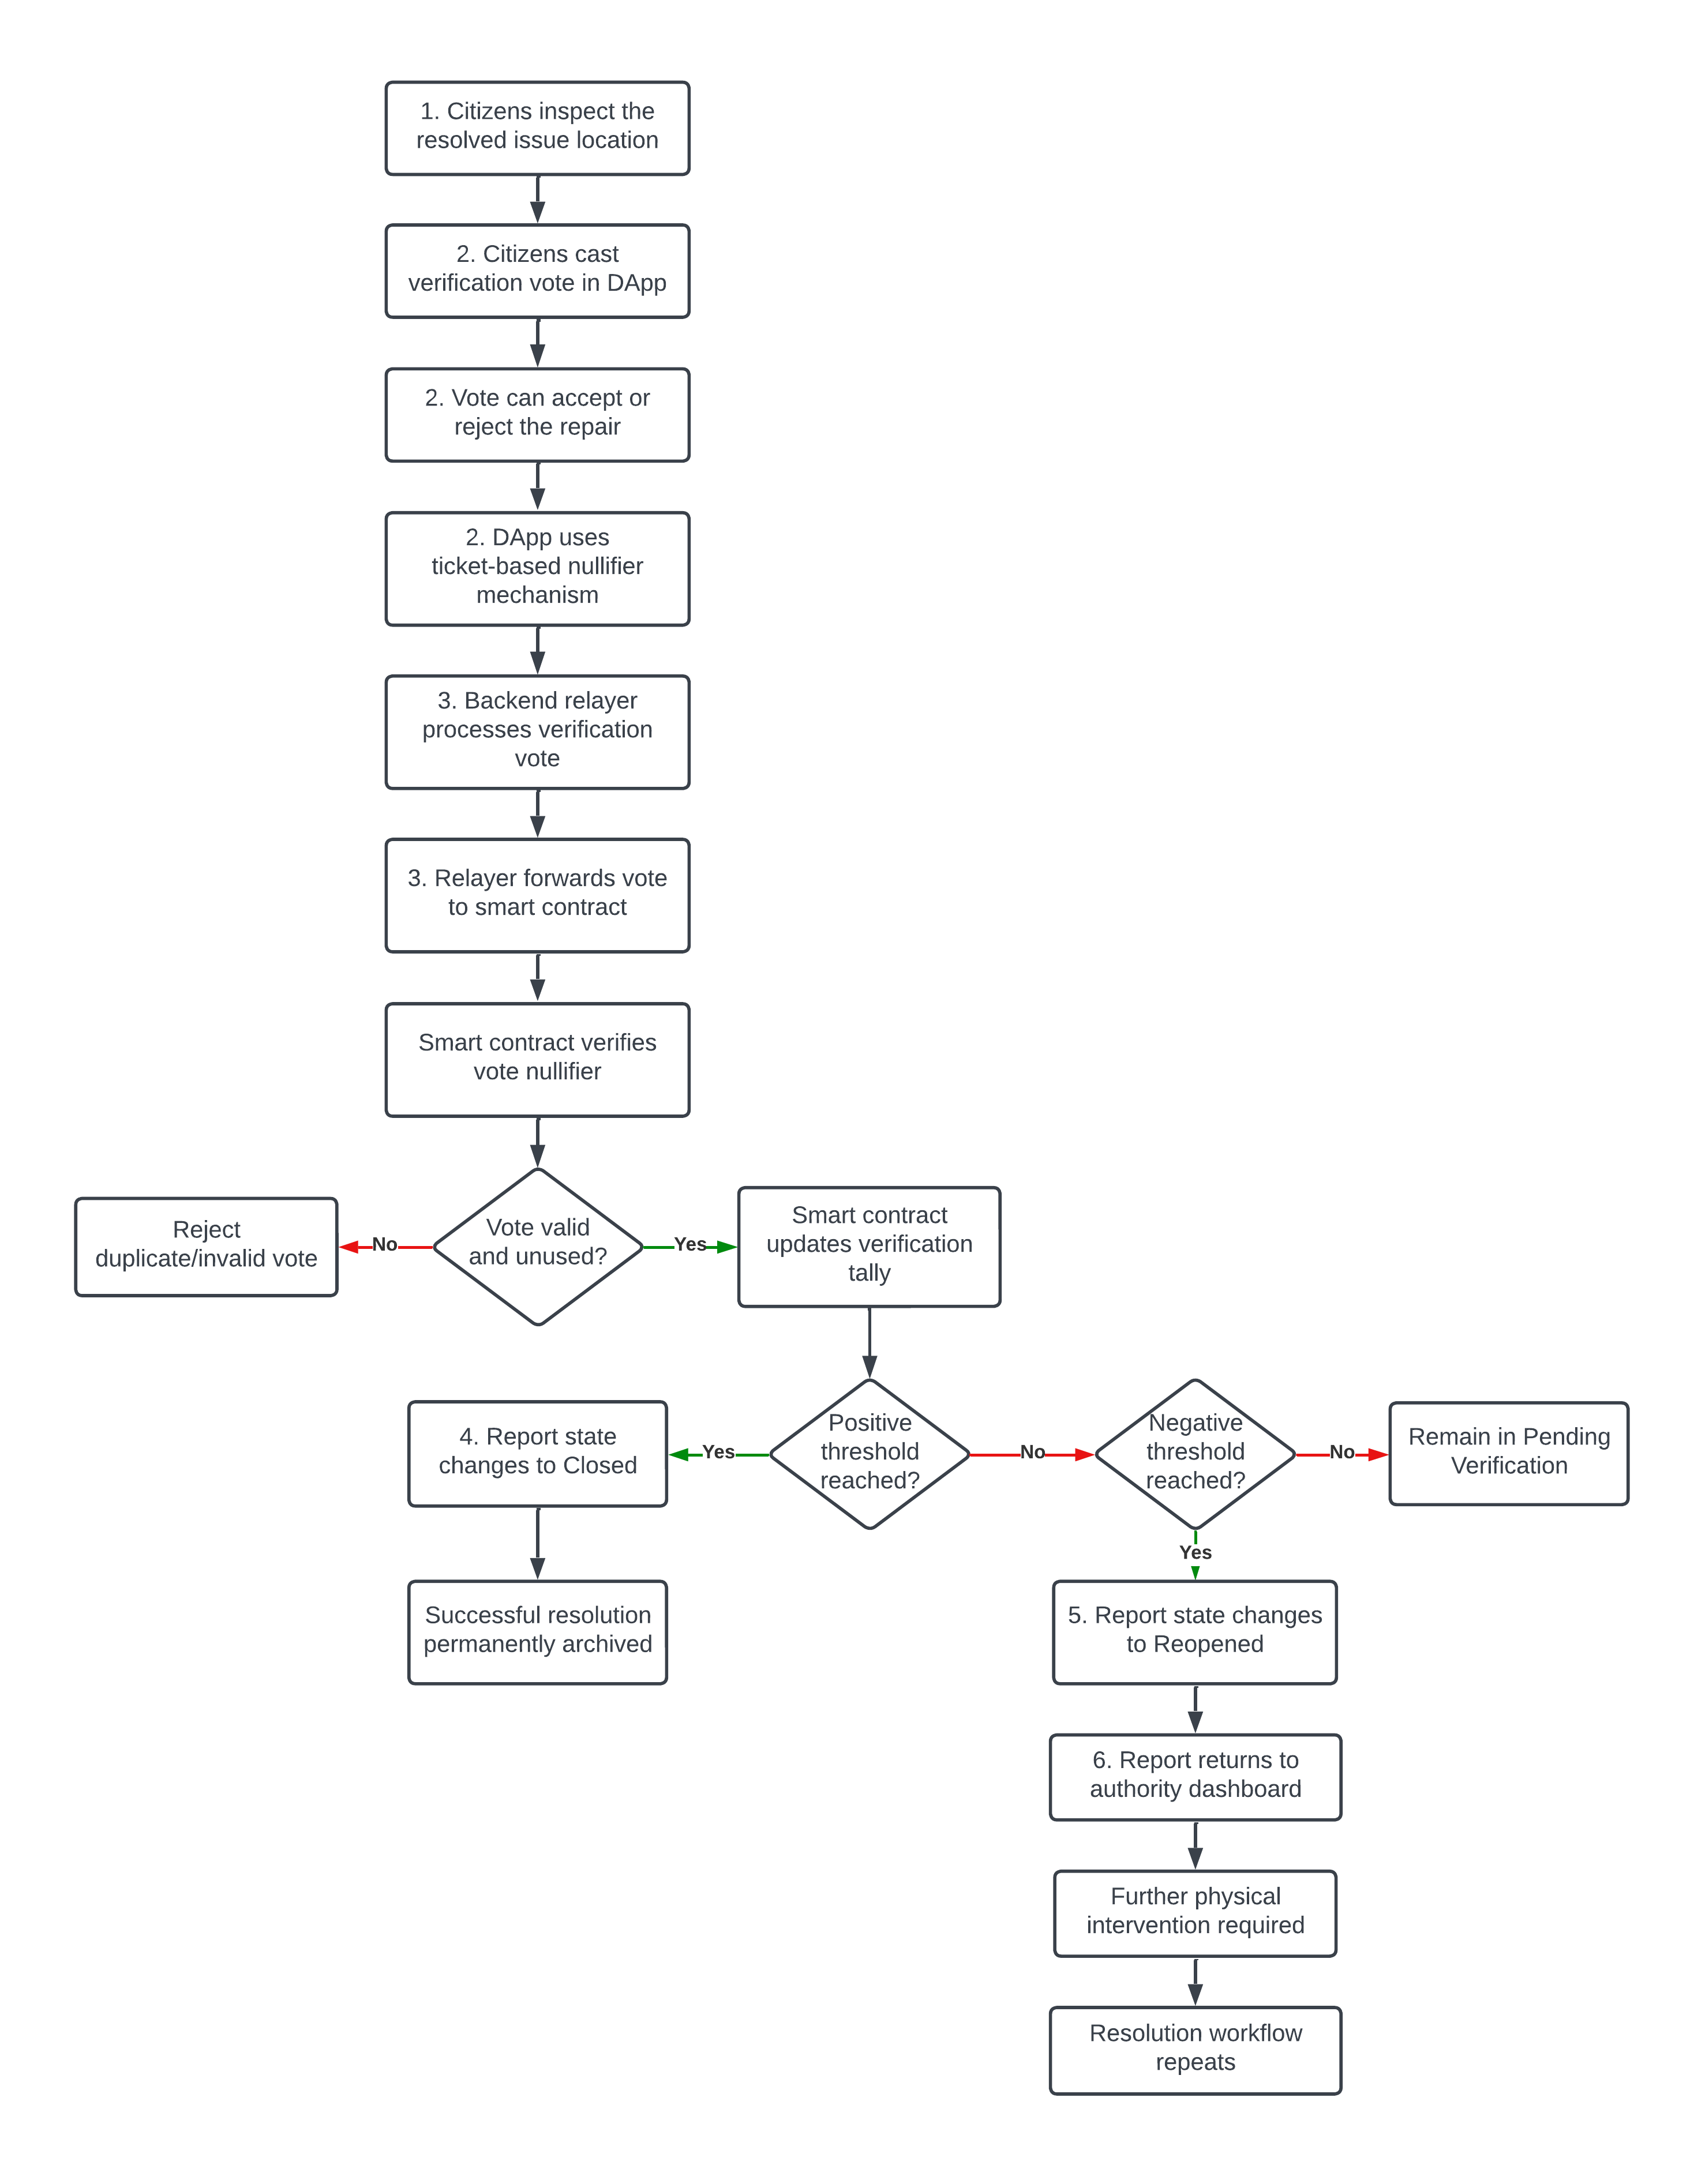
\includegraphics[width=0.95\textwidth,height=0.75\textheight,keepaspectratio]{Images/Chapter 3/post_resolution_verification_workflow.png}
%     \caption{Post-Resolution Verification and Community Appeal Workflow}
%     \label{fig:post-resolution-verification-workflow}
% \end{figure}

% The post-resolution workflow governs two distinct review paths:
% \begin{enumerate}
%     \item \textbf{Repair Verification ($S_5 = \texttt{PendingVerification}$):} The citizens will carry out a physical inspection of the completed repair work and then submit their acceptance ($\texttt{accept} = \text{true}$) or rejection ($\texttt{accept} = \text{false}$) votes by using the \texttt{castVerificationVote} function within the 6-hour period; when the deadline is reached:
%     \begin{itemize}
%         \item If the number of votes to accept the verification is greater than or equal to the number of votes to reject it ($\rho_{\text{accept}} \ge \rho_{\text{reject}}$), the report moves into the terminal state $S_6 (\texttt{Closed})$, which indicates that the issue has been successfully resolved.
%         \item If the number of verification reject votes is greater than the number of verification accept votes ($\rho_{\text{reject}} > \rho_{\text{accept}}$), the report is moved to $S_7 (\texttt{Reopened})$, which informs the municipal authorities that the repair was inadequate and needs corrective action.
%     \end{itemize}
%     \item \textbf{Rejection Review and Appeal ($S_4 = \texttt{PendingRejectionReview}$):} If an authority rejects an issue, the citizens then vote to either uphold ($\texttt{uphold} = \text{true}$) or to appeal ($\texttt{uphold} = \text{false}$) the rejection by using the \texttt{castRejectionReviewVote} function. When the deadline is finalised:
%     \begin{itemize}
%         \item If the number of votes in favour of upholding the rejection is greater than or equal to the number of votes in favour of appealing ($\upsilon_{\text{uphold}} \ge \upsilon_{\text{appeal}}$), then the rejection is upheld and the report moves to $S_6 (\texttt{Closed})$.
%         \item If the number of votes in favour of the appeal is greater than the number of votes upholding the rejection ($\upsilon_{\text{appeal}} > \upsilon_{\text{uphold}}$), then the community appeal is successful and the report moves to $S_7 (\texttt{Reopened})$, which requires the authority to re-examine the issue.
%     \end{itemize}
% \end{enumerate}

% \subsection{Anonymous Public Opinion Polling Workflow}
% \label{subsec:opinion-polling-workflow}

% Apart from the possibility of citizens reporting issues themselves, the system also provides for top-down municipal consultation via an anonymous public opinion polling procedure which is managed by the \texttt{OpinionPolling.sol} smart contract. This procedure allows local governments to obtain democratic feedback on proposals concerning public works, zoning changes, or budget allocations without compromising voter privacy

% The opinion polling workflow proceeds as follows:
% \begin{enumerate}
%     \item \textbf{Official Poll Creation:} To create an official poll, an authorized municipal official calls the \texttt{createOfficialPoll(ipfsMetadataCid, deadline, pollType)} function, providing as parameters the \ac{IPFS} \ac{CID} which holds the detailed documentation of the proposal, the deadline timestamp, and the type of poll (either \texttt{TrueFalse} or \texttt{MultiChoice}). The smart contract then checks the official's authority credentials against the access registry in \texttt{Reporting.sol}, assigns a unique \texttt{pollId}, and triggers the \texttt{PollCreated} event.
%     \item \textbf{DApp Poll Dissemination:} When it comes to the distribution of \ac{DApp} polls, the selectable voting options are shown on the citizen's \ac{DApp} interface together with the details of the proposals retrieved from \ac{IPFS}.
%     \item \textbf{Anonymous Ballot Casting:} When a citizen wants to cast an anonymous ballot, they choose an option index and produce a voting request which is then signed using an unused ticket nullifier. The relayer then submits the transaction to the \texttt{castVote(pollId, optionIndex, nullifier)} function.
%     \item \textbf{Sybil-Resistant Tallying:} The smart contract checks whether \texttt{nullifierVoted[pollId][nullifier]} has been consumed; if it has not been consumed, it records the nullifier and increases \texttt{pollResults[pollId][optionIndex]}.
%     \item \textbf{Poll Finalization:} Once the deadline elapses, any user or relayer can call \texttt{finalizePoll(pollId)} to mark the poll inactive and freeze results, providing municipal authorities with immutable, tamper-evident public consultation data.
% \end{enumerate}

% \section{Summary and Expected Outcomes}
% \label{sec:summary-outcomes}

% This chapter sets out the structural architecture, the interface specifications, the mathematical modelling of the state, the two-tier multi-signature governance, and the operational workflows of the decentralised local governance reporting framework. Through the use of a six-layer topology together with a hybrid on-chain/off-chain execution model, the system manages to overcome the main limitations of traditional centralised reporting systems.

% The expected outcomes of the architectural design include:
% \begin{enumerate}
%     \item \textbf{Guaranteed Citizen Anonymity and Privacy:} Citizens' anonymity and privacy are guaranteed since zero-knowledge authentication and single-use ticket nullifiers fully separate their real-world identity from the transactions on the chain, thus eliminating the fear of retaliation.
%     \item \textbf{Decentralized Municipal Governance:} By introducing \texttt{AuthorityMultiSig.sol}, decentralized municipal governance is achieved, so that access to authority and official identity profiles is controlled democratically by a majority quorum of the Super Admins.
%     \item \textbf{Automated Off-Chain Orchestration:} The relayer's automated \texttt{AuthorityFundingService} and \texttt{CronService} remove the need for manual treasury management and make it possible to deterministically finalise batches of expired voting windows.
%     \item \textbf{Tamper-Evident Accountability:} Ensuring tamper-evident accountability consists of storing metadata, records of state transitions, logs of authority actions, and the voting tallies on a private \ac{PoA} blockchain so that an immutable audit trail is obtained.
%     \item \textbf{Automated Spam and Toxicity Mitigation:} The multi-oracle \ac{AI} Moderation Ensemble prevents abusive, irrelevant, or malicious content from polluting off-chain storage or ledger state.
%     \item \textbf{Democratic Lifecycle Oversight:} There should be oversight of the democratic lifecycle by means of community voting which is resistant to Sybil attacks at the stages of validation, verification, and appeal, in order to prevent the arbitrary dismissal of reports and to ensure that repairs meet a certain standard.
%     \item \textbf{High Usability and Gasless Interaction:} The middleware relayer pattern eliminates cryptocurrency onboarding barriers, allowing citizens to engage via a responsive web application seamlessly.
% \end{enumerate}

% With the system architecture, mathematical state machine, governance topology, and workflows fully specified, Chapter 4 presents the technical realization and code-level implementation of each architectural component.
